\documentclass[11pt, a4paper, openany]{book}

% Règles de bonne pratiques :
% https://fr.wikibooks.org/wiki/LaTeX/Gestion_des_gros_documents

%%%%%%%%%%%%%%%%
%%% Packages %%%
%%%%%%%%%%%%%%%%

%%% Compatibilité %%%
\begingroup\expandafter\expandafter\expandafter\endgroup
\expandafter\ifx\csname IncludeInRelease\endcsname\relax
\usepackage{fixltx2e}
\fi 					% Si version LaTeX < 2015, inclut un fix.

%%% Général %%%
\usepackage[utf8]{inputenc}
\usepackage[british,french]{babel}
\usepackage[T1]{fontenc}
%\addto\extrasfrench{\sisetup{locale = FR,detect-all}} % Switch siunitx en fonction de la langue babel :)
%\addto\extrasbritish{\sisetup{locale = UK,detect-all}}
\usepackage{mathpazo}
\usepackage{lmodern}
\usepackage{courier}
\usepackage{graphicx}
\usepackage{cancel}

%%% Tableau %%%
\usepackage{tabularx} %Permet d'auto dimensionner les tableaux



%%% Bibliographie %%%
\usepackage[style=alphabetic,backend=biber]{biblatex}
\usepackage[autostyle]{csquotes}
\DeclareNameAlias{sortname}{last-first}
\DeclareFieldFormat{url}{\space\url{#1}}
\DeclareNameAlias{labelname}{last-first}
%\addbibresource{sample.bib}


%%% Graphiques %%%
\usepackage{tikz}
\usepackage{pgfplots}
\usepackage{circuitikz}

%%% Mise en page %%%
\usepackage{amsmath}
\usepackage{amsfonts}
\usepackage{amssymb}
\usepackage{amsthm}
\usepackage[tt]{titlepic}% Centre le titre
\usepackage{fancyhdr}   % Permet de modifier l'entête & footer
\usepackage{caption}     % Permet d'ajouter des légendes en images sans les mettre en float + dans la marge + ref vers le haut de l'envirronement
\usepackage{wrapfig}
\usepackage{fullpage}
\usepackage{multicol}   % pour les liste sur plusieurs colonnes
\usepackage{subfigure}  % alligne deux images cote a cote
\usepackage{float}      %permet de mettre du texte entre les figures grace a [H]. Génial! 
\usepackage{eso-pic}    % Fond d'écran page de garde
\usepackage{adjustbox}  % Empêche les box de sortir de la page


%%% Math %%%
\usepackage{delarray} % Belles matrices
\usepackage{siunitx}
\sisetup{locale = FR,detect-all}

% Pour mettre siunitx en mode français (virgule plutôt que point etc.)

%%% Codes %%%
\usepackage{listings}
\usepackage[final]{pdfpages} %% Inclusion fichier pdf

%% Reference
\usepackage{hyperref}
\renewcommand*{\figureautorefname}{fig.}
\def\appendixautorefname{annexe}
\def\tableautorefname{tab.}
\renewcommand*{\chapterautorefname}{ch.}
\newcommand{\subfigureautorefname}{\figureautorefname}



%%%%%%%%%%%%%%%%%
%%% Commandes %%%
%%%%%%%%%%%%%%%%%

%%% Physique %%%
\newcommand{\cst}{\text{cst}}
\newcommand{\D}{\partial}
\newcommand{\E}{\vec E}
\newcommand{\B}{\vec B}
\newcommand{\F}{\vec F}
\newcommand{\modu}[1]{|$#1$|}

%%% Math %%%
\newcommand{\oiint}{\int\!\!\!\!\!\!\! \:\!\subset\!\!\supset\!\!\!\!\!\!\!\int}
\newcommand{\rot}{\text{rot}\,}
\newcommand{\divv}{\text{div}\,}
\newcommand{\phas}[1]{\underline{#1}}
\newcommand{\RE}{\text{Re}}
\newcommand{\ft}{\overset{\mathcal{F}}{\longleftrightarrow}}
\newcommand{\lt}{\overset{\mathcal{L}}{\longleftrightarrow}}
\newcommand{\DS}{\displaystyle}



%% Box
\newcommand{\theor}[1]{\adjustbox{minipage=\linewidth-2\fboxsep-2\fboxrule,fbox}{\textsc{Théorème : }#1}}
\newcommand{\defi}[1]{\adjustbox{minipage=\linewidth-2\fboxsep-2\fboxrule,fbox}{\textsc{Définition : }#1}}
\newcommand{\lemme}[1]{\adjustbox{minipage=\linewidth-2\fboxsep-2\fboxrule,fbox}{\textsc{Lemme : }#1}}
\newcommand{\prop}[1]{\adjustbox{minipage=\linewidth-2\fboxsep-2\fboxrule,fbox}{\textsc{Propriété}\\ #1}}
\newcommand{\proposition}[1]{\adjustbox{minipage=\linewidth-2\fboxsep-2\fboxrule,fbox}{\textsc{Proposition}\\#1}}
\newcommand{\retenir}[1]{\adjustbox{minipage=\linewidth-2\fboxsep-2\fboxrule,fbox}{\textbf{\textit{\textsc{À retenir} : }}#1}}
\newcommand{\corollaire}[1]{\ \\\begin{tabular}{||c}
	\begin{minipage}{\textwidth}
		\textsc{Corollaire : } \textit{#1}
	\end{minipage}
	\end{tabular}}
\newcommand{\exemple}[1]{\ \\\begin{tabular}{|c}
	\begin{minipage}{\textwidth}
		\textsc{Exemple : } #1
	\end{minipage}
	\end{tabular}}
    
    

%\pagestyle{headings} % Titre du ch et numéro page dans l'entete
\renewcommand{\proofname}{Démonstration}
\selectlanguage{french}
\addto\captionsfrench{\def\tablename{Tableau}}


%%% Background %%%
\newcommand\BackgroundPic{%
	\put(0,0){%
		\parbox[b][\paperheight]{\paperwidth}{%
			\vfill
			\centering
			\includegraphics[width=\paperwidth,height=\paperheight,%
			keepaspectratio]{../../Builder/ulb.jpg}%
			\vfill
}}}

%%% Annexes Cedu %%%
%\usepackage{calrsfs}
\DeclareMathAlphabet{\pazocal}{OMS}{zplm}{m}{n}
\usepackage{fourier-orns}

\setlength{\parindent}{0pt} 

%%% Attributs %%%
\newcommand*{\NomduCours}[2]{\def\cours{#1}\def\memo{#2}}
\newcommand*{\auteur}[2]{\def\prenom{#1}\def\nom{#2}}
\newcommand*{\noteur}[2]{\def\nprenom{#1}\def\nnom{#2}}
\newcommand*{\rappeltheo}[2]{\def\rappeltheoprenom{#1}\def\rappeltheonom{#2}}
\newcommand*{\professeur}[2]{\def\pprenom{#1}\def\pnom{#2}}
\newcommand*{\sprofesseur}[2]{\def\spprenom{#1}\def\spnom{#2}}
\newcommand*{\annee}[2]{\def\adebut{#1}\def\afin{#2}}

% Attributs
\NomduCours{Power electronics}{ELEC-H-312}
\auteur{Enes}{Ulusoy}
\professeur{Johan}{Gyselink}
\annee{2015}{2016}

% Document
\begin{document}
\def\equationautorefname~#1\null{%
	(#1)\null
}


%%%%%%%%%%%%%%%%%
% Préliminaires %
%%%%%%%%%%%%%%%%%
\frontmatter
\begin{titlepage}
\begin{center}

% Upper part of the page. The '~' is needed because \\
% only works if a paragraph has started.

\includegraphics[width=0.6\textwidth]{logoulb2}~\\[1cm]

\textsc{\LARGE Université libre de Bruxelles}\\[1.5cm]

\textsc{\Large Groupe I}\\[1cm]
\textsc{\LARGE ELEC-H-200}\\[0.5cm]
% Title
\HRule \\[0.4cm]
{ \LARGE \textbf{Rapport de laboratoire}\\ Tous les labos ont obtenus le maximum }

\HRule \\[1cm]
% Auteurs
Terence \textsc{Blesin}\hspace{1cm}  Nicolas \textsc{Englebert}\hspace{1cm}  Benoît \textsc{Vernier}
% Bas de page
\vfill

{\large 2014 - 2015}



\end{center}
\end{titlepage}
\chapter*{Appel à contribution}
\subsection*{Synthèse Open Source}
\begin{wrapfigure}[5]{l}{4.5cm}
	\includegraphics[scale=0.5]{../../Builder/git.png}
\end{wrapfigure}
Ce document est grandement inspiré de l’excellent cours donné 
par \pprenom~\pnom\	
\ifdefined\spprenom
et\ \spprenom~\spnom\ 
\fi
 à l’EPB (École Polytechnique de Bruxelles), faculté de l’ULB (Université 
Libre de Bruxelles). Il est écrit par les auteurs susnommés avec l’aide de tous les autres étudiants 
et votre aide est la bienvenue ! En effet, il y a toujours moyen de l’améliorer surtout que si le 
cours change, la synthèse doit être changée en conséquence. On peut retrouver le code source à l’adresse 
suivante
\begin{center}
	\url{https://github.com/nenglebert/Syntheses}
\end{center}\ \\
Pour contribuer à cette synthèse, il vous suffira de créer un compte sur \textit{Github.com}. De
légères modifications (petites coquilles, orthographe, ...) peuvent directement être faites sur le
site ! Vous avez vu une petite faute ? Si oui, la corriger de cette façon ne prendra que quelques 
secondes, une bonne raison de le faire ! \\
\\
Pour de plus longues modifications, il est intéressant de disposer des fichiers : il vous 
faudra pour cela installer \LaTeX, mais aussi \textit{git}. Si cela pose problème, nous sommes 
évidemment ouverts à des contributeurs envoyant leur changement par mail ou n’importe quel autre 
moyen.\\
\\
Le lien donné ci-dessus contient aussi un \texttt{README} contenant de plus amples informations, 
vous êtes invités à le lire si vous voulez faire avancer ce projet ! 

\subsection*{Licence Creative Commons}
\begin{wrapfigure}[3]{r}{2.8cm}
	\vspace{-5mm}
	\includegraphics[scale=0.17]{../../Builder/CC}
\end{wrapfigure}
Le contenu de ce document est sous la licence Creative Commons : \textit{Attribution-NonCommercial-ShareAlike 
4.0 International (CC BY-NC-SA 4.0)}. Celle-ci vous autorise à l'exploiter pleinement, compte-
tenu de trois choses :
\begin{enumerate}
	\item \textit{Attribution} ; si vous utilisez/modifiez ce document vous devez signaler le(s) nom(s)
	      de(s) auteur(s).
	\item \textit{Non Commercial} ; interdiction de tirer un profit commercial de l’œuvre sans 
	      autorisation de l'auteur 
	\item \textit{Share alike} ;  partage de l’œuvre, avec obligation de rediffuser selon la même 
	      licence ou une licence similaire
\end{enumerate}
Si vous voulez en savoir plus sur cette licence :
\begin{center}
	\url{http://creativecommons.org/licenses/by-nc-sa/4.0/}
\end{center}

\begin{flushright}
	\textbf{Merci ! }
\end{flushright}
\tableofcontents
%Si abstract, \input ici

%%%%%%%%%%%%%%%%%%%%%
% Contenu principal %
%%%%%%%%%%%%%%%%%%%%%
\mainmatter
\chapter{Notation de Dirac}
\section{Vecteurs d'état et espace de Hilbert}
Le \textit{vecteur d'état} se dénomme \textit{ket} et est noté :
\begin{equation}
\begin{array}{ll}
\ket{\psi} & \in \mathcal{E}\\
&\in \mathcal{E}_H
\end{array}
\end{equation}
où $\mathcal{E}$ est l'espace des états et $\mathcal{E}_H$ l'espace de Hilbert. 
Notons que $\mathcal{E} \subset \mathcal{E}_H$. Par abus de langage, nous 
désignerons souvent l'espace des états comme étant l'espace de Hilbert, ce qui 
n'est en toute rigueur pas exact ($\mathcal{E}_H$ contient des états non-physiques).
L'espace de Hilbert est un espace complet (si on définit une suite d'état, celle-ci 
convergera vers un état) muni d'un produit scalaire (défini à la section suivante).\\

Pourquoi définir un vecteur d'état ? En physique classique l'état d'un système 
ne pose pas de problème particulier. A l'inverse, en physique quantique, la notion 
même d'état pose déjà un problème, contraignant l'utilisation de vecteurs d'état. La raison 
physique de leur utilisation vient du principe d'incertitude d'Heisenberg. En effet, 
il nous est impossible de décrire la particule par le couple position/impulsion d'où 
la motivation à l'utilisation de ces vecteurs.\\

A la base de la physique, le \textbf{principe de superposition} nous dit que la 
combili (de coefficients complexes) de deux vecteurs d'états, soit deux kets, est 
de nouveau un ket, soit un état 100\% admissible.
\begin{equation}
\ket{\psi_1}, \ket{\psi_2} \in\mathcal{E},\qquad \ket{\lambda_1\psi_1+\lambda_2\psi_2} 
\equiv \lambda_1\ket{\psi_1}+\lambda_2\ket{\psi_2}\qquad \forall \lambda_1,\lambda_2\in
\mathbb{C}
\end{equation}
Il s'agit de la \textit{linéarité de la physique quantique} avec laquelle on peut, par 
exemple, décrire le phénomène d'interférences.


\section{Produit scalaire entre deux kets}
Le produit scalaire entre deux kets se note
\begin{equation}
\bra{\psi_2}\ket{\psi_1}
\end{equation}
\newpage
Les propriétés de bases de ce produit scalaires sont bien connues :
\begin{equation}
\begin{array}{llll}
\bullet & \bra{\psi}\ket{\psi} &> 0\\
\bullet & \bra{\psi_1}\ket{\psi_2} &= \bra{\psi_2}\ket{\psi_1}^*\\
\bullet & \bra{\psi}\ket{\lambda_1\psi_1+\lambda_2\psi_2} &= \lambda_1\bra{\psi_1}\ket{\psi_2}
+\lambda_2\bra{\psi_1}\ket{\psi_2}\quad \forall \lambda_i\in\mathbb{C}.\quad
& \text{Linéarité (à gauche)}\\
\bullet & \bra{\lambda_1\psi_1+\lambda_2\psi_2}\ket{\psi} &= \bra{\psi}\ket{\lambda_1
\psi_1+\lambda_2\psi_2}^* \quad & \text{Antilinéarité (à gauche)}\\
&  &= (\lambda_1\bra{\psi}\ket{\psi_1}+\lambda_2\bra{\psi}\ket{\psi_2})^*\\
&  &= \lambda_1^*\bra{\psi_1}\ket{\psi} +  \lambda_2^*\bra{\psi_2}\ket{\psi}\\
\bullet & \|\psi\| = \|\ket{\psi}\| = \sqrt{\bra{\psi}\ket{\psi}}>0
\end{array}
\end{equation}

Il est intéressant de s'intéresser à la \textit{"représentation"} d'un ket au sein 
d'un espace de Hilbert. Considérons l’exemple suivant (qui reviendra souvent).\\

\textsc{Exemple}\\
Considérons un espace de Hilbert de dimension $n$. Les vecteurs d'états, les ket, ne sont rien 
d'autres que des vecteurs colonnes dans cet espace de dimension $n$. Soit
\begin{equation}
\ket{u} = \left(\begin{array}{c}
u_1\\
u_2\\
\vdots\\
u_n
\end{array}\right),\qquad\qquad \ket{v} = \left(\begin{array}{c}
v_1\\
v_2\\
\vdots\\
v_n
\end{array}\right),\qquad u_i,v_i\in\mathbb{C}
\end{equation}
Le produit scalaire entre ces deux ket est donné par
\begin{equation}
\bra{v}\ket{u} = \sum_{i=1}^n v_i^*u_i = \underbrace{(v_1^*\ v_2^*\ \dots\ v_n^*)}_{(*)}
\left(\begin{array}{c}
u_1\\
u_2\\
\vdots\\
u_n
\end{array}\right)
\end{equation}
On va définir $(*)$ comme étant l'objet dual \textit{"complémentaire au ket"}, $\bra{v}$ que l'on 
nomme \textit{bra}. Ce bra appartient à un espace dual, ce qui est le sujet de la 
section suivante.


\section{Espace dual $\mathcal{E}^*$, vecteur "bra"}
Le bra est une forme linéaire : c'est une application qui va de l'espace des état 
(ou de Hilbert, pas de différence dans ce cours) vers l'ensemble des nombres complexes.
\begin{equation}
\varphi : \ket{\psi}\in\mathcal{E} \leadsto \varphi(\ket{\psi})\ \in \mathbb{C}
\end{equation}
Cette forme linéaire fait correspondre à chaque état un nombre complexe. La superposition 
est également vérifiée d'où le "linéaire".
\begin{equation}
\varphi(\ket{\lambda_1\psi_1 + \lambda_2\psi_2}) = \lambda_1\varphi(\ket{\psi_1})+
\lambda_2\varphi(\ket{\psi_2})\qquad \forall \lambda_1,\lambda_2\in\mathbb{C}
\end{equation}
où $\varphi \in \mathcal{E}^*$.\\

Il semble dès lors intéressant d'introduire un nouvel "objet" : 
\begin{equation}
\left\{\begin{array}{ll}
\varphi \in \mathcal{E}^*\\
\bra{\varphi}
\end{array}\right.
\end{equation}
Il s'agit de l'ensemble de toutes les formes linéaires, ensemble qui forme un espace dual. 
L'intérêt de ces nouveaux objets réside dans un isomorphisme : on associe à ket de l'espace des états 
un et un seul bra de l'espace dual.\\

Ceci étant dit, il faut caractériser et montrer comment cette application agit sur les espaces. 
\begin{equation}
\forall \ket{\psi} \in \mathcal{E},\qquad \underline{\varphi(\ket{\psi}) =\bra{\varphi}\ket{\psi}}
\end{equation}

L'avantage de cette notation est qu'elle permet deux visions complémentaires des choses :
soit on voit cela comme un produit scalaire entre deux kets, soit on voit cela comme une
forme linéaire, le bra, s'appliquant à un ket.\\

ON PEUT ENLEVER LE PARAGRAPHE SUIVANT ?

Cette application peut ainsi être écrite comme un produit scalaire. Il s'agit de la forme 
linéaire $\varphi$ qui s'applique à $\psi$ et qui donne un nombre complexe. Il existe une 
autre façon de voir ceci. On peut le voir comme le produit scalaire entre deux ket ou encore 
comme un bra (forme linéaire qui appliquée à un ket qui donnera un complexe) et un ket.\\
 
Comme précisé, il s'agit d'une forme \textbf{linéaire} :
\begin{equation}
\begin{array}{ll}
\varphi(\ket{\lambda_1\psi_1+\lambda_2\psi_2}) &= \bra{\varphi}\ket{\lambda_1\psi_1+\lambda_2\psi_2}\\
&= \lambda_1\bra{\varphi}\ket{\psi_1}+\lambda_2\bra{\varphi}\ket{\psi_2}\\
&= \lambda_1\varphi(\ket{\psi_1})+\lambda_2\varphi(\ket{\psi_2})
\end{array}
\end{equation}
L'espace dual est également un espace de Hilbert : toutes les propriétés de 
linéarité seront retrouvées. Ainsi, toute combili (complexe) de forme 
apparentent à $\mathcal{E}^*$ forme une troisième forme appartenant à 
$\mathcal{E}^*$.
\begin{equation}
\text{Si } \bra{\varphi_1},\bra{\varphi_2}\in\mathcal{E}^*, \text{ alors }\ 
\lambda_1\bra{\varphi_1} + \lambda_2\bra{\varphi_2} \in\mathcal{E}^*\qquad 
\forall \lambda_i\in\mathbb{C}
\end{equation}
On peut ainsi démontrer que $\mathcal{E}^*$ est un espace vectoriel.
Un bra se définit par son action sur tout ket :
\begin{equation}
\begin{array}{ll}
\forall \ket{\psi} : (\lambda_1\bra{\varphi_1} + \lambda_2\bra{\varphi_2})\ket{\psi} 
&= \lambda_1\bra{\varphi_1}\ket{\psi}+\lambda_2\bra{\varphi_2}\ket{\psi} \\
&= \lambda_1\bra{\psi}\ket{\varphi_1}^*+\lambda_2\bra{\psi}\ket{\varphi_2}^*\\
&= (\lambda_1^*\bra{\psi}\ket{\varphi_1}+\lambda_2^*\bra{\psi}\ket{\varphi_2})^*\\
&= \bra{\psi}\ket{\lambda_1^*\varphi_1+\lambda_2^*\varphi_2}^*\\
&= \bra{\lambda_1^*\varphi_1+\lambda_2^*\varphi_2}\ket{\psi}
\end{array}
\end{equation}
Nous avons donc bien un espace vectoriel (ce qui est clairement visualisable 
dans l'équation ci-dessous). La dernière relation applique un certain bra à 
n'importe que $\psi$. En terme de bra, on peut alors écrire
\begin{equation}
\underline{\lambda\bra{\varphi_1} + \lambda_2\bra{\varphi_2} = \bra{\lambda_1^*\varphi_1
+\lambda_2^*\varphi_2}}\qquad \lambda_1,\lambda_2\in\mathbb{C}
\end{equation}


On vient de voir qu'à n'importe quel bra je peux associer un ket. Il serait 
dès lors intéressant de trouver le ket correspondant à ce bra. Mais avant, on va définir 
la notion d'opérateur s'appliquant dans l'espace de Hilbert. \\

Il est possible de se représenter de façon plus précise ce qu'est un bra en 
se souvenant de l'exemple donné avec un espace de Hilbert de dimension $n$. Dans 
un tel espace, un bra n'est qu'un vecteur ligne complexe conjugué.

\subsection{Opérateurs linéaires (agissant dans $\mathcal{E}$)}
Un opérateur linéaire est une application qui fait correspondre un ket à un ket, à 
la différence de la forme qui fait correspondre un complexe à un ket.

\begin{equation}
\ket{\psi} \in \mathcal{E} \leadsto \hat{A}\ket{\psi} \in \mathcal{E}
\end{equation}
Il est coutume d'indiquer les opérateurs linéaires par un chapeau. La sainte 
superposition reste d'actualité :
\begin{equation}
\hat{A}\ket{\lambda_1\psi_1+\lambda_2\psi_2} = \lambda_1\hat{A}\ket{\psi_1}+
\lambda_2\hat{A}\ket{\psi_2}
\end{equation}
Pas mal de propriétés valent la peine d'être énoncées :
\begin{equation}
\begin{array}{llll}
\bullet & (\hat{A}+\hat{B})\ket{\psi} &= \hat{A}\ket{\psi}+\hat{B}+\ket{\psi}\\
\bullet & (\hat{A}.\hat{B})\ket{\psi} &= \hat{A}(\hat{B}\ket{\psi})\qquad & \text{ Opérateur 
produit $\hat{A}.\hat{B}$}
\end{array}
\end{equation}
Nous pouvons voir cet opérateur produit comme une notation efficace. Il ne faut 
cependant pas perdre à l'idée que, en toute généralité, $\hat{A}$ et $\hat{B}$ 
ne commutent pas. On définit alors le commutateur :
\begin{equation}
[\hat{A},\hat{B}] = \hat{A}\hat{B} - \hat{B}\hat{A}
\end{equation}
Comme $\hat{A}$ et $\hat{B}$ sont des opérateurs, la différence des opérateurs 
est toujours un opérateur, le commutateur est bien un opérateur. Il jouit des 
propriétés suivantes :
\begin{equation}
\begin{array}{lll}
\bullet & [\hat{B},\hat{A}] &= -[\hat{A},\hat{B}]\\
\bullet & [\hat{A},\hat{B}+\hat{C}] &= [\hat{A},\hat{B}]+[\hat{A},\hat{C}]\\
\bullet & [\hat{A},\hat{B}.\hat{C}] &= \hat{B}.[\hat{A},\hat{C}]+[\hat{A},
\hat{B}].\hat{C}
\end{array}
\end{equation}
On peut montrer qu'un opérateur linéaire peut se représenter comme une 
matrice. Pour l'illustrer, reconsidérons notre précédent exemple.\\

\textsc{Exemple}\\
Soit un espace de Hilbert de dimension finie $n$. Soit
\begin{equation}
\ket{u} = \left(\begin{array}{c}
u_1\\
u_2\\
\vdots\\
u_n
\end{array}\right),\qquad \ket{v} = \hat{A}\ket{u}\quad ; \left(\begin{array}{c}
v_1\\
v_2\\
\vdots\\
v_n
\end{array}\right) = \underbrace{\left(\begin{array}{ccc}
a_{11} & \dots & a_{1n}\\
\vdots &\ddots &\vdots\\
a_{n1} & \dots & a_{nn}
\end{array}\right)}_{\hat{A}}\left(\begin{array}{c}
u_1\\
u_2\\
\vdots\\
u_n
\end{array}\right)
\end{equation}

Le fait que le commutateur entre deux opérateurs soit non-nul indique que le
produit entre les matrcies correspondantes est non-commutatif.\\

De par cette représentation, on peut aisément comprendre que la non-commutation 
vient du fait que les différentes lignes et colonnes de $\hat{A}$ ne peuvent 
être commutées. Intéressons-nous aux éléments de la matrice de cet opérateur.



\section{"Élément de matrice" d'un opérateur $\hat{A}$}

Soient
\begin{equation}
\ket{\psi} \text{ et } \left\{\begin{array}{ll}
\ket{\varphi} &\in \mathcal{E}\\
\bra{\varphi} &\in \mathcal{E}^*
\end{array}\right.,
\end{equation}
comme précédemment, définissons un nouvel "objet" :
\begin{equation}
 \quad \bra{\varphi}\hat{A}\ket{\psi} = \bra{\varphi}(
\hat{A}\ket{\psi}) = (\bra{\varphi}\hat{A})\ket{\psi}
\end{equation}

%Les parenthèses permettent de voir ça "tel un produit scalaire". Revenons 
%à notre précédent problème : quel est finalement ce ket ? Lors de l'écriture 
%d'un élément de matrice, il est intéressant de pouvoir le voir comme un 
%opérateur appliqué à un ket. Une autre vision est celle d'un opérateur 
%qui agit sur un bra, définissant un nouveau bra qui cette fois, agit sur 
%$\psi$. Revenons à notre exemple.\\

FORMULATION BIZARRE, JE ME SUIS PERMIS DE CHANGER\\

Ce nouvel objet peut se comprendre de deux manières : on peut le voir comme
un opérateur s'appliquant à un ket pour former un nouveau ket que l'on
multiplie scalairement avec un bra, ou on peut le voir comme un opérateur
agissant sur un bra pour former une nouvelle forme qui s'appliquera au ket $\psi$.
Notons qu'en réalité il ne s'agit pas du même opérateur car les espaces vectoriels
de départ et d'arrivée ne ont pas les mêmes dans les deux cas. Cependant ils possèdent
la même forme en représentation matricielle et l'abus de notation est très pratique.
Notons également qu'un opérateur est entièrement caractérisé par ses éléments de matrice.\\

Revenons à notre exemple.

%\newpage
\textsc{Exemple}\\
Soit
\begin{equation}
\ket{u} = \left(\begin{array}{c}
u_1\\
u_2\\
\vdots\\
u_n
\end{array}\right), \qquad \bra{v} = (v_1^*\ v_2^*\ \dots\ v_n^*), \qquad 
\hat{A}\ket{u} = \left(\begin{array}{ccc}
a_{11} & \dots & a_{1n}\\
\vdots &\ddots &\vdots\\
a_{n1} & \dots & a_{nn}
\end{array}\right)\left(\begin{array}{c}
u_1\\
u_2\\
\vdots\\
u_n
\end{array}\right)
\end{equation}
Nous avons alors
\begin{equation}
\bra{v}\left(\hat{A}\ket{u}\right) = \underbrace{(v_1^*\ v_2^*\ \dots\ v_n^*)\left(\begin{array}{ccc}
a_{11} & \dots & a_{1n}\\
\vdots &\ddots &\vdots\\
a_{n1} & \dots & a_{nn}
\end{array}\right)}_{\bra{?}\ket{u}}\left(\begin{array}{c}
u_1\\
u_2\\
\vdots\\
u_n
\end{array}\right)
\end{equation}

\begin{equation}
\bra{v}\left(\hat{A}\ket{u}\right) = (v_1^*\ v_2^*\ \dots\ v_n^*)\underbrace{\left(\begin{array}{ccc}
a_{11} & \dots & a_{1n}\\
\vdots &\ddots &\vdots\\
a_{n1} & \dots & a_{nn}
\end{array}\right)\left(\begin{array}{c}
u_1\\
u_2\\
\vdots\\
u_n
\end{array}\right)}_{\left(\hat{A}\ket{u}\right)}\\
\end{equation}



\section{Opérateur adjoint}
A tout opérateur $\hat{A}$, on peut associer un nouvel opérateur noté $\hat{A}^\dagger$ (prononcé "dagger"). 
Soit $\ket{\psi}$ :
\begin{equation}
\hat{A} \text{ agit dans }\mathcal{E} ; \ket{\psi'} = \hat{A}\ket{\psi}
\label{eq:16}
\end{equation}
Chaque ket est associé à un bra ; dans ce cas ci il s'agit de $\bra{\psi'}$ et
$\bra{\psi}$. Existe-t-il une relation entre ces bra ? Mais à quoi cet objet 
correspond-t-il ? Un bra est une forme linéaire, il faut déterminer comment 
agit $\bra{\psi'}$ sur n'importe quel ket de l'espace.
\begin{equation}
\begin{array}{lll}
\forall \ket{\phi} \in \mathcal{E} : \bra{\psi'}\left(\ket{\varphi}\right) &\equiv 
\bra{\psi'}\ket{\varphi} & \qquad \text{Prop. p.scal.}\\
&= \bra{\varphi}\ket{\psi'}^*\\
&= \bra{\varphi}\hat{A}\ket{\psi}^* & \qquad \text{Def. de }\psi', \text{ def. op. adj.}\\
&= \bra{\psi}\hat{A}^\dagger\ket{\varphi}& \qquad \text{(*)}
\end{array}
\end{equation}
Pour arriver à $(*)$, on peut remplacer $\hat{A}$ par son adjoint si l'on 
permute les termes et considère le complexe conjugué.
La conclusion de tous cela - modulo la définition de l'opérateur adjoint - est 
que l'on voit que l'on peut réécrire le $\bra{\psi'}$ en terme de $\bra{\psi}$.
\begin{equation}
\underline{\bra{\psi'} = \bra{\psi}\hat{A}^\dagger}
\end{equation}
Cette relation ressemble assez fortement à \autoref{eq:16} ou $\hat{A}\rightarrow
\hat{A}^\dagger$.
De façon générale on peut voir qu'un opérateur linéaire peut être entièrement 
caractérisé par ses éléments de matrice, exactement comme une matrice est 
caractérisée par tous ses éléments. Pour parvenir à ce résultat, nous avons 
utilisé la définition d'un opérateur adjoint :
\begin{equation}
\forall \ket{\psi} \text{ et } \ket{\varphi} \in \mathcal{E},\qquad 
\bra{\psi}\hat{A}^\dagger \ket{\varphi} = \bra{\psi}\hat{A}\ket{\varphi}^*
\end{equation}

\textsc{Exemple}\\
Comme toujours, prenons notre espace de Hilbert de dimension finie $n$.
\begin{equation}
\bra{v}\hat{A}\ket{u} = \underbrace{(v_1^*\ v_2^*\ \dots\ v_n^*)\left(\begin{array}{ccc}
a_{11} & \dots & a_{1n}\\
\vdots &\ddots &\vdots\\
a_{n1} & \dots & a_{nn}
\end{array}\right)}_{(*)}\left(\begin{array}{c}
u_1\\
u_2\\
\vdots\\
u_n
\end{array}\right)
\end{equation}
Le "but" est que $(*)$ devienne notre nouveau bra $(w_1\ w_2\ \dots\ w_n)$ :
\begin{equation}
\left(\begin{array}{c}
w_1\\
w_2\\
\vdots\\
w_n
\end{array}\right) = \underbrace{\left(\begin{array}{ccc}
a_{11}^* & \dots & a_{1n}^*\\
\vdots &\ddots &\vdots\\
a_{n1}^* & \dots & a_{nn}^*
\end{array}\right)}_{\hat{A}^\dagger}\left(\begin{array}{c}
v_1\\
v_2\\
\vdots\\
v_n
\end{array}\right)
\end{equation}
%Pour obtenir le bra, nous avons réalisé une opération semblable à celles 
%réalisées en algèbre linéaire, à savoir pris le complexe conjugé de la matrice 
%conjugué après inversion et transposée du vecteur.\footnote{Mieux expliciter plz}.

JE ME SUIS PERMIS DE REFORMULER.\\

Pour obtenir le bra, nous avons utilisé une méthode semblable à celle
réalisée en algèbre linéaire : nous avons obtenu la matrice de l'opérateur
adjoint en prenant la transposée de la matrice conjuguée.
L'opérateur adjoint n'est rien d'autre que la matrice adjointe.
Notons que la conjugaison et la transposition ne dépendent que de la base
choisie et que l'existence de l'opérateur adjoint est garantie si on peut l'obtenir
dans au moins une base. Le fait de permuter les lignes et les colonnes ne faisait 
qu'inverser les bra et ket.\\
Il en découle des propriétés intéressantes :
\begin{multicols}{2}
\begin{itemize}
\item[$\bullet$] $\left(\hat{A}^\dagger\right)^\dagger = \hat{A}$
\item[$\bullet$] $\left(\lambda\hat{A}\right)^\dagger = \lambda^*\hat{A}$
\item[$\bullet$] $\left(\hat{A}+\hat{B}\right)^\dagger = \hat{A}^\dagger+\hat{B}^\dagger$
\item[$\bullet$] $\left(\hat{A}.\hat{B}\right) = \hat{B}^\dagger.\hat{A}^\dagger$
\end{itemize}
\end{multicols}
A titre d'exercice, démontrons la dernière propriété
\begin{equation}
\begin{array}{ll}
\bra{\psi}\left(\hat{A}.\hat{B}\right)^\dagger\ket{\varphi} &= \bra{\varphi}\hat{A}.
\hat{B}\ket{\psi}^*\\
&= \left(\left(\bra{\varphi}\ket{\hat{A}}\right)\left(\bra{\hat{B}}\ket{\psi}\right)\right)^*\\
&= (\bra{\psi}\hat{B}^\dagger)(\hat{A}^\dagger\ket{\varphi})\\
&= \bra{\psi}\hat{B}^\dagger\hat{A}^\dagger\ket{\varphi}
\end{array}
\end{equation}

\section{Opérateurs hermitiens/auto-adjoints}
Par définition, $\hat{A}$ est auto-adjoint si
\begin{equation}
\hat{A} = \hat{A}^\dagger
\end{equation}
Dès lors
\begin{equation}
\begin{array}{ll}
\bra{\psi}\hat{A}\ket{\varphi} &= \bra{\varphi}\hat{A}\ket{\psi}^*\\
\bra{\psi}\hat{A}\ket{\psi} &= \bra{\psi}\hat{A}\ket{\psi}^* \rightarrow \underline{\in \mathbb{R}}
\end{array}
\end{equation}
Énonçons quelques propriétés intéressantes\footnote{Les opérateurs de quantités observables sont
auto-adjoints.}
\begin{equation}
\begin{array}{lll}
\forall \hat{A},\hat{B} \text{ hermitiens },\qquad & \hat{A}+\hat{B} & \text{hermitien}\\
& \hat{A}.\hat{B} & \text{hermitien ssi } [\hat{A},\hat{B}] = 0
\end{array}
\end{equation}
On peut justifier la dernière propriété de la façon suivante :
\begin{equation}
\begin{array}{lll}
(\hat{A}.\hat{B})^\dagger &= \hat{B}^\dagger.\hat{A}^\dagger \\
&= \hat{A}^\dagger.\hat{B}^\dagger & \text{vrai ssi } [\hat{A}^\dagger,\hat{B}^\dagger]=0=-
\underbrace{[\hat{A},\hat{B}]^\dagger}_{=0}\\
&= \hat{A}.\hat{B}
\end{array}
\end{equation}
Le produit position et impulsion n'est pas un opérateur hermitien (ces deux états ne 
commutent pas) ; ce n'est donc pas une quantité observable en physique quantique.\\




%COURS 2
%%%%%%%%%%%%%%%%%%%%%%%%%%%%%%%%%%%%%%%%%%%%%%%%%%%%%%%%%%%%%%%%%%%%%%%%%%%%%%%%%%%%%
Pour obtenir le complexe conjugué avec les notations de Dirac, il suffit de lire à 
l'envers pour obtenir ce que l'on souhaite :
\begin{equation}
\begin{array}{ll}
\hat{A}\ket{\psi} &\rightarrow \bra{\psi}\hat{A}^\dagger\\
\bra{\varphi}\hat{B}&\rightarrow \hat{B}^\dagger \ket{\varphi}\\
\bra{\psi}\hat{A}\ket{\varphi} &\rightarrow  \bra{\varphi}\hat{A}^\dagger\ket{\psi} =
\bra{\psi}\hat{A}\ket{\varphi}^*
\end{array}
\end{equation}
Un autre exemple, un peu moins trivial est de considérer l'opérateur suivant
\begin{equation}
\ket{u}\bra{v} \rightarrow (\ket{u}\bra{v})^\dagger= \ket{v}\bra{u}
\end{equation}
Avec la notation $\ket{u}\bra{v}\ket{\varphi}$, on se rend 
compte qu'il s'agit bien d'un opérateur agissant sur l'état $\ket{\varphi}$. Afin de 
s'en rendre compte, développons ceci à titre d'application
\begin{equation}
\begin{array}{lll}
\bra{\varphi}\underline{\left(\ket{u}\bra{v}\right)^\dagger}\ket{\psi} &= (\bra{\psi}(\ket{u}\bra{v})
\ket{\varphi})^* & (*)\\
&=(\bra{\psi}\ket{u})^*(\bra{v}\ket{\varphi})^*\\
&=(\bra{u}\ket{\psi})(\bra{\varphi}\ket{v})\\
&=(\bra{\varphi}\ket{v})(\bra{u}\ket{\psi}) & \text{Commutativité}\\
&=\bra{\varphi}\underline{(\ket{v}\bra{u})}\ket{\psi}
\end{array}
\end{equation}
Il est possible de voir $(*)$ de deux façons différentes. On peut le comprendre comme 
un objet (opérateur) dont on prend l'élément de matrice entre $\psi$ et $\varphi$ (comme 
le suggère les parenthèses). On peut également le voir comme deux produits scalaire dont 
on fait le produit simple (en omettant cette fois-ci les parenthèses).


\subsection{Base Hilbertienne}
Une base hilbertienne est une base de l'espace de Hilbert. Il en existe deux types particuliers:
la base discrète de dimension finie et la base continue.

\subsubsection{Base discrète}
Nous parlons de l'espace de Hilbert et donc d'un espace des états, soit encore un ensemble 
de ket qui sous-tendent l'espace :
\begin{equation}
\left\{\ket{u_i}\right\}
\end{equation}
Ces vecteurs de base sont orthonormés
\begin{equation}
\bra{u_i}\ket{u_j} = \delta_{ij}
\end{equation}
Le but d'une telle base est d'exprimer n'importe quel ket, n'importe quel état, comme une 
combili des vecteurs de cette base. En toute généralité, on peut écrire un ket comme une 
somme sur $i$ de coefficients multiplicatifs $C_i$ (qui joueront le rôle d'amplitude de 
probabilité, mais ils sont avant tout des coefficients de Fourier)
\begin{equation}
\ket{\psi} = \sum_i C_i\ket{u_i}
\label{eq:2.5}
\end{equation}
En remarquant que
\begin{equation}
\bra{u_j}\ket{\psi} = \sum_iC_i\underbrace{\bra{u_j}\ket{u_i}}_{\delta_{ij}} = C_j
\end{equation}
On peut réécrire \autoref{eq:2.5} :
\begin{equation}
\begin{array}{lll}
\ket{\psi} &= \sum_i \bra{u_i}\ket{\psi}\ket{u_i} & \text{Notations de Dirac}\\
&= \sum_i \ket{u_i}\bra{u_i}\ket{\psi} & \text{(Somme d') Op. lin. appliqué(e) à $\psi$}\\
&\underbrace{\left(\sum_i \ket{u_i}\bra{u_i}\right)}_{\mathbb{1}}\ket{\psi} & \forall\psi
\end{array}
\end{equation}

On voit apparaître la relation de fermeture. Dès que l'on a une base complète, la somme des projecteurs
$\ket{u_i}\bra{u_i}$ donnera l'opérateur identité. On appelle alors la \textbf{relation 
de fermeture} :
\begin{equation}
\sum_i \ket{u_i}\bra{u_i} = \hat{\mathbb{1}}
\end{equation}
On peut alors définir l'opérateur \textit{projecteur} $\hat{P_i}$ :
\begin{equation}
\hat{P_i} = \ket{u_i}\bra{u_i}
\end{equation}
Cet opérateur possède deux propriétés remarquables. La première est qu'il est hermitien, 
c'est-à-dire $\hat{P_i} = \hat{P_i}^\dagger$.
\begin{equation}
\hat{P_i}^\dagger = (\ket{u_i}\bra{u_i})^\dagger = \ket{u_i}\bra{u_i} = \hat{P_i}
\end{equation}
La seconde est qu'il est idempotent. Autrement dit, plus d'une application successive ne 
change rien au résultat obtenu : $\hat{P_i}^2 = \hat{P_i}$.
\begin{equation}
\begin{array}{ll}
\hat{P_i}^2 &= (\ket{u_i}\bra{u_i})(\ket{u_i}\bra{u_i})\\
&= \ket{u_i}\underbrace{\bra{u_i}\ket{u_i}}_{=1}\bra{u_i}\\
&= \hat{P_i}
\end{array}
\end{equation}
On interprète le projecteur comme on le ferait dans l'espace euclidien\footnote{Inclure 
graphe}. La relation de fermeture peut ainsi être réécrite :
\begin{equation}
\sum_i \hat{P_i} = \hat{\mathbb{1}}
\end{equation}
Le développement suivi ici est valable pour toute base. Prenons l'exemple d'un ket
\begin{equation}
\text{ket }\ \ket{\psi} = \sum_i c_i\ket{u_i},\qquad c_i = \bra{u_i}\ket{\psi}
\end{equation}
On peut faire de même pour un bra. Pour définir un bra, il faut premièrement définir 
un ket puis prendre son élément dual.
\begin{equation}
\begin{array}{lll}
& \ket{\varphi} &= \sum_i b_i\ket{u_i},\qquad b_i = \bra{u_i}\ket{\varphi}\\
\text{bra } & \bra{\varphi} &= \sum_i b_i^* \bra{u_i}
\end{array}
\end{equation}
Comment faire pour exprimer un produit scalaire ? Il suffit de faire apparaître 
l'opérateur identité et jouer avec les notations de Dirac
\begin{equation}
\begin{array}{lll}
\bra{\varphi}\ket{\psi} &= \bra{\varphi}\mathbb{1}\ket{\psi}\\
&= \sum_i \underbrace{\bra{\varphi}\ket{u_i}}_{b_i^*}\underbrace{\bra{u_i}\ket{\psi}}_{c_i} &
\text{Relation de fermeture}\\
&= \sum_i b_i^*c_i & (*)
\end{array}
\end{equation}
Dans $(*)$, $b_i^*$ est un vecteur ligne et $c_i$ un vecteur colonne. Si l'espace de Hilbert 
est complet, il s'agit là d'un produit scalaire.\\
Cela fonctionne également pour un opérateur, en effectuant la même astuce mathématique:
\begin{equation}
\begin{array}{ll}
\hat{A} &= \hat{\mathbb{1}}\hat{A}\hat{\mathbb{1}}\\
&=\sum_{i,j} \ket{u_i}\underbrace{\bra{u_i}\hat{A}\ket{u_j}}_{A_{i,j}}\bra{u_j}
\end{array}
\end{equation}
Appliquons $\hat{A}$ sur un ket
\begin{equation}
\begin{array}{ll}
\ket{\psi'} &= \hat{A}\ket{\psi}\\
&\equiv \sum_i a_i\ket{u_i}
\end{array},\qquad \begin{array}{ll}
a_i &= \bra{u_i}\ket{\psi'}\\
&=\bra{u_i}\hat{A}\mathbb{1}\ket{\psi} = \sum_j \underbrace{\bra{u_i}\hat{A}\ket{u_j}}_{A_{i,j}}
\underbrace{\bra{u_j}\ket{\psi}}_{c_j}
\end{array}
\end{equation}
où l'on a utilisé $\ket{\psi'} = \hat{A}\ket{\psi}$ et $a_i = \sum_jA_{ij}c_j\  "=" 
\left(\begin{array}{c}
\vdots\\
\vdots\\
\vdots
\end{array}\right) = \left(\begin{array}{ccc}
  & \dots &  \\
\vdots &\ddots &\vdots\\
  & \dots &  
\end{array}\right)\left(\begin{array}{c}
\vdots\\
\vdots\\
\vdots\\
\end{array}\right)$.


\subsubsection{Base continue}
On va ici partir d'une famille ou cette fois ci l'indice sera "continu". 
\begin{equation}
\{\ket{u_\alpha}\}\quad \alpha\in\mathbb{R}
\end{equation}
On peut comme précédemment fabriquer des états orthogonaux. Ce qui va jouer 
le rôle orthonormalisation standard est le relation
\begin{equation}
\underline{\bra{u_\alpha}\ket{u_{\alpha'}} = \delta(\alpha-\alpha')}
\end{equation}
où $\delta$ est la fonction de Dirac. La subtilité est que $u_\alpha$ n'est 
pas toujours un état physique\footnote{La fonction de Dirac étant un pic de hauteur infinie
mais d'aire unitaire, il est difficile de la retrouver dans la nature...}.
 Cependant, il peut toujours être utilisé pour 
décrire un état qui lui, est bien physique. Comme pour le cas continu, il 
est possible d'exprimer le ket dans la base. Les sommes seront ainsi 
remplacées par es intégrales et les coefficients de Fourier par une fonction 
jouant le même rôle.
\begin{equation}
\ket{\psi} = \int d\alpha\ C(\alpha)\ket{u_\alpha}
\label{eq:2.12}
\end{equation}
où les $C(\alpha)$ renseignent sur le poids. Il est possible, comme précédemment, 
de déterminer ceux-ci en multipliant ce ket par un autre élément de la base.
\begin{equation}
\bra{u_{\alpha'}}\ket{\psi} = \int d\alpha\ C(\alpha) \underbrace{
\bra{u_{\alpha'}}\ket{u_\alpha}}_{=\delta(\alpha-\alpha')} = C(\alpha')
\end{equation}
On peut alors ré-écrire \autoref{eq:2.12}
\begin{equation}
\begin{array}{ll}
\ket{\psi} &= \int d\alpha\ \bra{u_\alpha}\ket{\psi}\ket{u_\alpha}\\
&= \int d\alpha\ \ket{u_\alpha}\bra{u_\alpha}\ket{\psi}\\
&=\displaystyle\left(\int d\alpha\ \ket{u_\alpha}\bra{u_\alpha}\right)\ket{\psi}
\qquad \forall\psi
\end{array}
\end{equation}
Le terme entre parenthèse n'est, par identification, rien d'autre que l'opérateur 
identité $\hat{\mathbb{1}}$ que l'on peut également voir comme un opérateur projecteur
$\hat{P_\alpha}$. La relation de fermeture s'écrit alors
\begin{equation}
\int d\alpha\ \underbrace{\ket{u_\alpha}\bra{u_\alpha}}_{\hat{P_\alpha}} = \hat{
\mathbb{1}}
\end{equation}
Comme nous l'avons fait pour le cas de la base discrète, montrons comment écrire 
un bra, ket, opérateur linéaire, \dots
\begin{equation}
\begin{array}{llll}
\text{ket } & \ket{\psi} &= \int d\alpha\ c(\alpha)\ket{u_\alpha} & \text{ où } 
c(\alpha) = \bra{u_\alpha}\ket{\psi}\\
& \ket{\varphi} &= \int d\alpha\ b(\alpha)\ket{u_\alpha} & \text{ où } b(\alpha) 
= \bra{u_\alpha}\ket{\varphi}\\
\text{bra } & \bra{\varphi} &= \int d\alpha\ b^*(\alpha)\bra{u_\alpha}
\end{array}
\end{equation}
Voyons maintenant pour le produit scalaire
\begin{equation}
\begin{array}{ll}
\bra{\varphi}\ket{\psi} = \bra{\varphi}\mathbb{1}\ket{\psi} &= \int d\alpha\ 
\underbrace{\bra{\varphi}\ket{u_\alpha}}_{b^*(\alpha)}\underbrace{\bra{u_\alpha}
\ket{\psi}}_{c(\alpha)}\\
&= \int d\alpha\ b^*(\alpha)c(\alpha)
\end{array}
\end{equation}
Par une analyse semblable pour les opérateurs. 
Définissons $\hat{A}$ :
\begin{equation}
\hat{A} = \mathbb{1}\hat{A}\mathbb{1} = \iint d\alpha\ d\alpha'\ \ket{u_\alpha}
\underbrace{\bra{u_\alpha}\hat{A}\ket{u_{\alpha'}}}_{A(\alpha,\alpha')}\bra{u_{\alpha'}}
\end{equation}
où $A(\alpha,\alpha')$ correspond aux éléments de matrice. \\
%Pour finir, intéressons nous au cas de l'opérateur adjoint\footnote{TT : détaille plus 
%ce qu'on essaye de montrer, c'est un peu pas clair :/}
Pour finir, examinons ce qui se passe quand on décompose en vecteurs de base un ket
auquel on a appliqué un opérateur :
\begin{equation}
\begin{array}{ll}
\ket{\psi'} = \hat{A}\ket{\psi} = \int d\alpha\ \overbrace{a(\alpha)}^{coef de Fourier}\ket{u_\alpha},
\qquad a(\alpha) &= \bra{u_\alpha}\ket{\psi'} = \bra{u_\alpha}\hat{A}\ket{\psi}\\
&= \int d\alpha'\ \underbrace{\bra{u_\alpha}\hat{A}\ket{u_{\alpha'}}}_{A(\alpha,
\alpha')}\underbrace{\bra{u_{\alpha'}}\ket{\psi}}_{c(\alpha')}
\end{array}
\end{equation}
%Nous nous intéressions à savoir ce qu'était $a(\alpha)$, c'est maintenant chose faite
On voit que le coefficient de Fourier du ket $\psi'$ est l'intégrale des produits des éléments de matrice
de l'opérateur avec les coefficient de Fourier du ket $\psi$ :
\begin{equation}
\underline{a(\alpha) = \int d\alpha'\ A(\alpha,\alpha')c(\alpha')}
\end{equation}
Dans le cas discret, nous avions $a_i = \sum_j A_{ij}c_j$. Ici le résultat est identique, 
mais sous forme intégrale. Cette expression illustre bien à quel point la notation de 
Dirac est compacte.


\subsection{Exemple de base de représentation continue : la base position}
Il existe bien évidemment plusieurs bases. L'une d'entre elles se nomme 
\textbf{base position}
\begin{equation}
\left\{\ket{\vec{r}}\right\}\qquad \vec{r}\in\mathbb{R}^3
\end{equation}
N'importe quel ket pourra s'exprimer dans cette base position. Le relation 
fermeture pour la base position nous dis que l'intégration sur tout l'espace
du projecteur pour une position donnée donnée l'identité.\footnote{Projeter
un ket sur un vecteur de la base position $\ket{r}$ revient quasiment à évaluer la 
probabilité que la particule se trouve au point r. On comprend intuitivement
que la particule doit se trouver quelque part dans l'espace et donc que
la somme des probabilités pour qu'elle se trouve en chacun des points doit
être égale à un.}
\begin{equation}
\int d\vec{r}\ \ket{\vec{r}}\bra{\vec{r}} = \vec{\mathbb{1}}
\end{equation}
Compte-tenu de cette relation, on peut exprimer les ket au moyen des $\ket{r}$
\begin{equation}
\ket{\psi} = \int d\vec{r}\ \ket{\vec{r}}\underbrace{\bra{\vec{r}}\ket{
\psi}}_{\psi(\vec{r})}
\end{equation}
où $\psi(\vec{r})$ est la \textit{fonction d'onde}\footnote{La fonction d'onde
utilisée en mécanique ondulatoire n'est donc rien d'autre que le "poids" qu'on associe
à chaque $\ket{r}$ quand on décrit l'état $\ket{\psi}$ de la particule. On retrouve
bien le fait que la fonction d'onde est liée à la probabilité qu'une particule se trouve
en un point de l'espace.}. En plaçant la relation 
d'identité à droite du bra, on obtient
\begin{equation}
\bra{\varphi} = \int d\vec{r}\ \underbrace{\bra{\varphi}\ket{\vec{r}}}_{
\varphi^*(\vec{r})}
\bra{\vec{r}}
\end{equation}
où $\varphi^*(\vec{r})$ est le complexe conjugué de la fonction d'onde du 
ket associé.
% En effet, nous avons\footnote{Dans quel but ? TT?}
Le produit scalaire entre deux vecteurs d'état devient donc :
\begin{equation}
\begin{array}{ll}
\bra{\varphi}\ket{\psi} = \bra{\varphi}\mathbb{1}\ket{\psi} &= \int d\vec{r}\ 
\bra{\varphi}\ket{\vec{r}}\bra{\vec{r}}\ket{\psi}\\
&= \int d\vec{r}\ \varphi^*(\vec{r})\psi(\vec{r})
\end{array}
\end{equation}
qui n'est rien d'autre que le produit scalaire usuel pour des fonctions complexes (cf cours
d'analyse).
Considérons le cas où $\ket{\psi}=\ket{\vec{r'}}$
% \footnote{TT : complète plz, j'sais plus pq on fait ça}
pour trouver la fonction d'onde correspondant à un vecteur de la base position.
\begin{equation}
\begin{array}{ll}
\ket{\vec{r'}} &= \displaystyle \int d\vec{r}\ \ket{\vec{r}}\underbrace{\bra{\vec{r}}\ket{\vec{r'}}}
_{\psi_{\vec{r'}}(\vec{r)}}\\
&\rightarrow\psi_{\vec{r'}}(\vec{r}) =\displaystyle \delta(\vec{r}-\vec{r'})
\end{array}
\end{equation}
Le delta de Dirac est dépourvu de sens physique, celui-ci représentant un étant 
infiniment localisé. Or, nous savons que de telle solutions divergent. Malgré tout, 
même sans être un état physique, 
il est pratique pour former une base.



\section{Observable}
Une \textit{observable} est un opérateur linéaire hermitien $\hat{A}$ associé à 
une grandeur physique observable $A$. A toute grandeur physique observable, il 
est possible de lui associer un opérateur linéaire  hermitien. Si $\ket{\psi}$
est un vecteur propre de $\hat{A}$,
\begin{equation}
\hat{A}\ket{\psi} = \lambda\ket{\psi}
\end{equation}
où $\lambda$ est une valeur propre pouvant être dégénérée (la dimension 
du sous-espace propre associé à $\lambda$ est appelée la \textit{dégénérescence}) 
ou non dégénérée.\\
Une classification importante se base sur le \textit{spectre}. Le spectre est
l'ensemble de toutes les valeurs propres possibles $\{\lambda\}$ de l'opérateur. Si celui-ci 
est discret, on retrouvera un système lié (particule dans une boîte par exemple). On 
peut également avoir des spectres continus (systèmes libres), utiles dans la 
\textit{théorie des collisions/diffusion}.\\

\subsubsection{Propriétés d'une observable}

%Intéressons-nous aux propriétés de notre base.
\begin{enumerate}
\item Toute valeur propre $\lambda$ est réelle.
\begin{equation}
\begin{array}{ll}
A\ket{\psi} &= \lambda \ket{\psi}\qquad\qquad\qquad \left(\hat{A}^\dagger = 
\hat{A}\right)\\
\bra{\psi}A\ket{\psi} = \lambda\underbrace{\bra{\psi}\ket{\psi}}_{=1}
\end{array}
\end{equation}
En prenant le complexe conjugué, on trouve
\begin{equation}
\lambda^* = \bra{\psi}A^\dagger\ket{\psi} = \bra{\psi}A\ket{\psi}=\lambda\in
\mathbb{R}
\end{equation}

\item Les vecteurs propres associés à deux valeurs propres distinctes sont 
orthogonaux.\\
Soit $\lambda_1\neq\lambda_2$
\begin{equation}
\left\{\begin{array}{ll}
A\ket{\psi_1} &=\lambda_1\ket{\psi_1}\\
A\ket{\psi_2} &=\lambda_2\ket{\psi_2}
\end{array}\right.
\end{equation}
En multipliant la première ligne par $\bra{\psi_2}$ et la seconde par $\bra{\psi_1}$
\begin{equation}
\left\{\begin{array}{ll}
\bra{\psi_2}A\ket{\psi_1} &=\lambda_1\bra{\psi_2}\ket{\psi_1}\\
\bra{\psi_1}A\ket{\psi_2} &=\lambda_2\bra{\psi_1}\ket{\psi_2}
\end{array}\right.
\label{eq:Syst}
\end{equation}
Considérons le complexe conjugué de la deuxième équation de \autoref{eq:Syst} 
\begin{equation}
\bra{\psi_2}A^\dagger\ket{\psi_1} = \lambda_2^*\bra{\psi_2}\ket{\psi_1}\qquad
\leftrightarrow
\qquad\bra{\psi_2}A\ket{\psi_1} = \lambda_2\bra{\psi_2}\ket{\psi_1}
\end{equation}
Le membre de gauche de cette expression est identique au membre de gauche de 
la première équation de \autoref{eq:Syst}. En effectuant la différence :
\begin{equation}
0 = (\lambda_1-\lambda_2)\bra{\psi_2}\ket{\psi_1},\qquad \lambda_1\neq\lambda_2 
\quad\Rightarrow\quad \bra{\psi_2}\ket{\psi_1} = 0
\end{equation}
\end{enumerate}
Dans le cas ou $\lambda_n$ est $g_n$ fois dégénérée, on utilisera la notation
\begin{equation}
\hat{A}\ket{\psi_n^i} = \lambda_n\ket{\psi_n^i}\qquad \lambda_n \rightarrow i=
1,2,\dots, g_n
\end{equation}
Ceci va nous amener à la décomposition spectrale des opérateurs ; il est 
toujours possible de les représenter dans une base. Une base particulièrement 
intéressante est celle composée des vecteurs propres de l'observable qui nous 
intéresse.

\subsubsection{Décomposition spectrale de A}
Comme introduit en fin de section précédente, deux indices sont utilisés : 
un pour désigner la valeur propre et l'autre pour la dégénérescence.
\begin{equation}
\hat{A}\ket{\psi_n^i} = \lambda_n\ket{\psi_n^i}\qquad \lambda_n \rightarrow i=
1,2,\dots, g_n
\end{equation}
La relation d'orthonormalité est toujours d'application
\begin{equation}
\bra{\psi_n^i}\ket{\psi_{n'}^{i'}} = \delta_{n,n'}\delta_{i,i'}
\end{equation}
Notons que l'algorithme de Gram-Schmidt permet de toujours pouvoir trouver une
base orthonormée au sein d'un sous-espace dégénéré.\\
Rappelons-nous que la relation de fermeture nous indique que si on somme les 
projecteurs sur tous les vecteurs de la base, on retrouvera l'identité. Dans 
notre cas, la relation de fermeture s'énonce (pour toute base, il 
est possible d'écrire une relation équivalente)
\begin{equation}
\sum_n\sum_{i=1}^{g_n} \ket{\psi_n^i}\bra{\psi_n^i} = \hat{\mathbb{1}}
\end{equation}

\textsc{Théorème de décomposition spectrale}\\
\begin{equation}
\begin{array}{ll}
\hat{A} &= \hat{A}\mathbb{1} = \sum_n\sum_{i=1}^{g_n} \hat{A}\ket{\psi_n^i
}\bra{\psi_n^i}\\
\hat{A} &= \sum_n \lambda_n \overbrace{\sum_{i=1}^{g_n} \ket{\psi_n^i}\bra{
\psi_n^i}}^{\text{Somme de proj. = proj.}}\\
\hat{A} &= \sum_n \lambda_n \hat{P}_n
\end{array}
\end{equation}
%mise en page un peu moche :(
où $\hat{P}_n$ est le projecteur sur le sous-espace propre de rang $g_n$ associé à $n$.
 Montrons que les $\hat{P}_n$ sont des projecteurs orthogonaux

\begin{equation}
\begin{array}{ll}
\hat{P_n}\ket{\psi^{i'}_{n'}} = \sum_n \sum_i \ket{\psi^i_{n}}
 \underbrace{\bra{\psi^i_{n}}\ket{\psi^{i'}_{n'}}}_{\delta_{n n'} \delta_{i i'}} 
= \delta_{n n'} \ket{\psi^{i'}_{n'}}\\
\hat{P_n}\hat{P_{n'}} = \sum_{i'} \hat{P_n} \ket{\psi^{i'}_{n'}}\bra{\psi^{i'}_{n'}}
 = \delta_{n n'} \sum_{i'}\ket{\psi^{i'}_{n'}}\bra{\psi^{i'}_{n'}}
 = \delta_{n n'}\hat{P_{n'}}\\
\rightarrow \hat{P_n}\hat{P_{n'}} = \delta_{n n'}\hat{P_{n'}}
\end{array}
\end{equation}




\textsc{Observable à spectre continu}\\
Considérons un triplet d'opérateur\footnote{Deuxième relation montre la valeur 
propre. L'intérieur du ket fait référence à la valeur propre associée.}
%On n'adopterait pas une autre notation pour désigner la valeur propre 
%(genre $\overline{r}$) ? Un peu ambigu.}
\begin{equation}
\hat{\vec{r}} = (\hat{x},\hat{y},\hat{z}),\qquad \hat{\vec{r}}\ket{\vec{r}} = 
\vec{r}\ket{\vec{r}}
\end{equation}
Effectuons la décomposition spectrale de $\hat{\vec{r}}$
\begin{equation}
\hat{\vec{r}} = \int d\vec{r}\ \vec{r}\ \ket{\vec{r}}\bra{\vec{r}}
\end{equation}
Ceci est l'intégrale d'un opérateur, donnant lieu à un opérateur (en réalité 
trois, car il s'agit d'un triplet d'opérateur).La décomposition spectrale peut 
s'écrire comme ceci. \\
A la place de l'opérateur $\hat{\vec r}$, considérons l'opérateur $\hat{\vec{\mathbb{1}}}$
 : comme il n'a que une seule valeur propre, nous retrouvons
\begin{equation}
\hat{\vec{\mathbb{1}}} = \int d\vec{r}\ \ket{\vec{r}}\bra{\vec{r}}
\end{equation}
Ceci montre que le relation de fermeture n'est rien d'autre que la 
décomposition spectrale d'un opérateur particulier.\\

La base impulsion est liée à la décomposition en valeur propre de l'opérateur 
impulsion (triplet d'opérateur) :
\begin{equation}
\hat{\vec{p}} = \left(\hat{p_x},\hat{p_y},\hat{p_z}\right),\qquad \hat{
\vec{p}}\ket{\vec{p}} = \vec{p}\ket{\vec{p}}
\end{equation}
Connaître exactement l'impulsion implique une position étalée sur l'infini 
d'énergie infinie, ce n'est pas physique.
\footnote{Phrase bizarre... En plus, on n'a pas encore parlé de l'incertitude
à ce stade-ci du cours...} 
Il est possible d'effectuer la décomposition spectrale
\begin{equation}
\hat{\vec{p}} = \int d\vec{p}\ \vec{p} \ket{\vec{p}}\bra{\vec{p}}
\end{equation}
La fonction d'onde peut elle aussi s'exprimer dans la base impulsion
\begin{equation}
\bra{\vec{p}}\ket{\psi}
\end{equation}

En réalité, les bases position et impulsion sont liées par une transformée de Fourier
et il est possible d'effecter le changement de base grâce à $\bra{\vec{r}}\ket{
\vec{p}})$ mais ceci fera l'objet d'un autre chapitre du cours.
%Il sera possible d'utiliser le changement de base de Fourier ($\bra{\vec{r}}\ket{
%\vec{p}})$ pour exprimer cette fonction d'onde dans la base position 
%$\bra{\vec{r}}\ket{\psi}$.\\

Afin d'introduire la notion d'\textit{ECOC}, rappelons la décomposition spectrale
\begin{equation}
\hat{A}\ket{\psi_n'} = a_n\ket{\psi_n'}\quad i=1,\dots,g_n\qquad\rightarrow\qquad
\hat{A} = \sum_na_n\hat{P_n}\quad\text{ où }\ \hat{P_n}=\sum_i\ket{\psi_n^i}\bra{
\psi_n^i}
\end{equation}
On peut montrer que \textit{lorsque les observables d'un ensemble commutent
deux à deux, il existe au moins une base de vecteurs propres communs à ces observables.} 
\begin{equation}
\left\{\hat{A},\hat{B},\hat{C},\dots\right\}\quad\rightarrow\quad \left\{n_a,
n_b,n_c,\dots\right\}
\end{equation}
où $n_a$ est le nombre quantique associé à $\hat{A}$, etc. Cette base de vecteurs
propres communs constituera une base privilégiée pour l'étude de problèmes
faisant intervenir cet ensemble d'observables. A priori, dans ces conditions,
la base obtenue ne sera pas forcément unique. On parle ainsi d'\textit{ECOC} 
(ensemble \textbf{complet} d'observables qui commutent deux à deux) : si la 
valeur propre de chacune des observable est fixée, il existe un unique état de 
la base. \\

Par exemple, si on étudie la dépendance angulaire
\begin{equation}
\left\{\hat{L}^2, \hat{L_z}\right\} \rightarrow \ket{l,m}
\end{equation}
Ces deux opérateurs commutent. On retrouve par ailleurs le nombre quantique 
orbital ainsi que le nombre quantique magnétique. Pour une particule dans un 
potentiel central 
\begin{equation}
\left\{\hat{H},\hat{L}^2, \hat{L_z}\right\} \rightarrow \ket{n_r,l,m}
\end{equation}
où $n_r$ est le nombre quantique radial associé à $\hat{H}$.
\chapter{La diffraction}
\begin{wrapfigure}[8]{r}{2cm}
\vspace{-6mm}
\includegraphics[scale=0.30]{ch2/image4.png}
\captionof{figure}{ }
\end{wrapfigure}
Un faisceau laser se propageant à tendance à s'élargir et se déformer : il s'agit du 
phénomène de diffraction. Ce phénomène est bien précis et peut être décrit mathématiquement. 
Il dépend notamment de la forme du laser. En faisant passer un laser par une section carrée, 
on sera amener à observer des distributions d'intensités particulières.

\section{Équations de Maxwell et transformée de Fourier}
La linéarité des équations de Maxwell permet un traitement efficace par les transformées 
de Fourier. Voici les fameuses équations dans le vide
\begin{equation}
\left\{\begin{array}{llll}
\rot \vec{E} &= -\dfrac{\partial \vec{B}}{\partial t},\qquad &\div \vec{E} &= 0\\
\rot \vec{B} &= \epsilon_0\mu_0\dfrac{\partial \vec{E}}{\partial t},\qquad &\div \vec{B} &= 0
\end{array}\right.
\end{equation}
Sachant que $\rot [\rot \vec{E}] = \grad[\div \vec{E}] - \Delta\vec{E}$ où $\div \vec{E}=0$ dans 
le vide on retrouve l'équation d'onde électromagnétique
\begin{equation}
\Delta \vec{E} = \mu_0\epsilon_0\dfrac{\partial^2\vec{E}}{\partial t^2}\quad \text{où } \Delta 
\vec{E} = \Delta E_x\vec{1_x}+\Delta E_y\vec{1_y}+\Delta E_z\vec{1_z}
\end{equation}
On ne considérera ici que la composante en $x$ du champ
\begin{equation}
\Delta E_x = \mu_0\epsilon_0\dfrac{\partial^2E_x}{\partial t^2}
\end{equation}
On remplacera souvent $E_x,E_y$ ou $E_z$ par $E$ mais il faut garder à l'idée qu'il ne s'agit 
qu'une seule des composantes du champ. L'équation d'onde scalaire s'écrit
\begin{equation}
\dfrac{\partial E}{\partial x^2}+\dfrac{\partial E}{\partial y^2}+\dfrac{\partial E}{\partial z^2} 
= \mu_0\epsilon_0\dfrac{\partial^2E}{\partial t^2}
\end{equation}
Cette équation est \textit{linéaire}, $E$ n'apparaissant qu'à la première puissance. Si $E_1$ et 
$E_2$ sont solution, une combili de ces deux solutions est également solution. On va profiter 
de cette linéarité pour exprimer la solution de cette équation comme une somme d'onde harmonique, 
d'où l'utilité des transformée de Fourier. Le champ électrique se verra décomposé en une somme 
de \textit{fonctions harmonique}\footnote{Écrit ci-dessous dans le domaine des phaseurs.} :
\begin{equation}
E(x,y,z,t) = \iiiint_{-\infty}^\infty \tilde{E}(k_x,k_y,k_z,\omega)e^{ik_xx}e^{ik_yy}e^{ik_zz}
e^{-i\omega t}\ dk_xdk_ydk_zd\omega
\end{equation}
Si le facteur harmonique $e^{ik_xx}e^{ik_yy}e^{ik_zz}e^{-i\omega t}$  est solution des équations 
de Maxwell $\forall k_i,\omega$, alors $E$ sera solution. La résolution de ces équations ne sont 
pas aisées. Pour le faire de façon analytique, on travaillera avec la décomposition. Vérifions 
que ces fonctions harmoniques sont bien solution
\begin{equation}
\dfrac{\partial^2 e^{ik_xx}e^{ik_yy}e^{ik_zz}e^{-i\omega t}}{\partial x^2} = -k_x^2 e^{ik_xx}e^{ik_yy}
e^{ik_zz}e^{-i\omega t}
\end{equation}
En faisant de même pour les deux autres dérivées partielles pour obtenir
\begin{equation}
(-k_x^2-k_y^2-k_z^2)e^{ik_xx}e^{ik_yy}e^{ik_zz}e^{-i\omega t} = -\mu_0\epsilon_0\omega^2 
e^{ik_xx}e^{ik_yy}e^{ik_zz}e^{-i\omega t}
\end{equation}
C'est-à-dire
\begin{equation}
k_x^2+k_y^2+k_z^2 = \mu_0\epsilon_0\omega^2
\end{equation}
Il s'agit d'une \textbf{contrainte} sur les modes de Fourier. On peut voir l'expression de $E$ 
comme une transformée de Fourier où $\tilde{E}$ est le spectre de Fourier généralisé à 4 
dimensions. En terme de transformée de Fourier, on peut dire qu'il s'agit d'une contrainte 
sur les \textit{modes de Fourier} (les quatre facteurs exponentiels), soit une \textbf{relation 
de dispersion généralisée}. Si les modes satisfont cette contrainte, $E$ sera solution.\\

\begin{wrapfigure}[9]{r}{3cm}
%\vspace{-6mm}
\includegraphics[scale=0.45]{ch2/image5.png}
\captionof{figure}{ }
\end{wrapfigure}
Intéressons-nous aux aspects physiques sous-jacent à cette décomposition de Fourier du champ 
électrique. Commençons par la ré-écriture suivante en supposant que les $k_i$ sont les 
composantes d'un vecteur
\begin{equation}
\tilde{E}(k_x,k_y,k_z,\omega)e^{ik_xx}e^{ik_yy}e^{ik_zz}e^{-i\omega t} = \tilde{E}(\vec{k},
\omega)e^{i\vec{k}.\vec{r}}e^{-i\omega t}
\end{equation}
\danger $\vec{r}$ est le vecteur position, il désigne le point de l'espace considéré. On peut 
ainsi exprimer la condition pour laquelle le mode de Fourier satisfait les équations de Maxwell  :
\begin{equation}
|k|^2 = k^2 = \mu_0\epsilon_0\omega^2
\end{equation}

\begin{wrapfigure}[9]{l}{3cm}
\vspace{-6mm}
\includegraphics[scale=0.45]{ch2/image6.png}
\captionof{figure}{ }
\end{wrapfigure}
Cela signifie que le vecteur d'onde est tendu d'être sur une sphère de rayon $k=
\sqrt{\mu_0\epsilon_0}\omega$. Figeons le temps et cherchons le lieux des points de phase 
constante. Pour avoir une phase constante, $\vec{k}.\vec{r}$ doit être constant : tous les 
points qui ont la même projection auront la même phase, il s'agit d'une \textit{onde plane}.
Ci-contre, la représentation des fronts d'ondes. Analysons cela de façon analytique
\begin{equation}
\varphi = \vec{k}.\vec{r} = \text{cste}\quad \Rightarrow k_xx+k_yy+k_zz = \text{ cste}
\end{equation}
Il s'agit de l’équation d'un plan perpendiculaire au vecteur d'onde. Les modes de Fourier 
réprésentent bien une onde plane dont la direction $\vec{k}/k$. On peut toujours considérer 
$\vec{k}/k = \vec{1_z} \rightarrow \vec{k}= k\vec{1_z}$ de sorte à écrire
\begin{equation}
E = \tilde{E}e^{ikz}e^{-i\omega t}
\end{equation}
Ceci montre que lorsque $z$ est fixé, le champ ne varie pas en $x$. Si l'on considère la 
partie réelle de ceci, on retrouve $\tilde{E}\cos(kz-\omega t)$ ce qui est bien l'équation 
d'une onde plane.\\

Que se passe-t-il si on libère le temps? Intéressons-nous d'abord à la périodicité en 
$z : \lambda = 2\pi/k$ ce qui correspond à l'espacement des fronts d'ondes. Considérons 
une phase constante
\begin{equation}
\text{Front d'onde : } \varphi = \text{ cste} \Rightarrow  kz-\omega t = \text{ cste} \qquad 
\Longleftrightarrow z = \dfrac{\omega}{k}t+\dfrac{\text{cste}}{k}
\end{equation}
Pour garder la constante, quand le temps augmente $z$ doit également augmenter. On obtient 
ici la \textit{vitesse de phase} $\omega/k = v_\phi$ où $k = \sqrt{\mu_0\epsilon_0}\omega$. 
Cette dernière condition est obligatoire pour avoir quelque chose de physique vérifiant 
les équations de Maxwell. Par substitution
\begin{equation}
v_\varphi = \dfrac{1}{\sqrt{\mu_0\epsilon_0}} \equiv c
\end{equation}
On en tire que $k=\omega/c$.\\

\underline{Remarque}. Considérons un champ scalaire solution des équations d'ondes 
\begin{equation}
\vec{E} = (A_x\vec{1_x}+A_y\vec{1_y}+A_z\vec{1_z})e^{ikz}e^{ikz}e^{-i\omega t}
\end{equation}
où les amplitudes $A_i$ ne sont pas nécessairement connues. Nous allons voir qu'il y a 
une contrainte sur ces amplitudes. Appliquons la divergence nulle du champ électrique 
dans le vide
\begin{equation}
\div \vec{E} = 0 \quad \Longrightarrow\quad \dfrac{\partial E_x}{\partial x}+
\dfrac{\partial E_y}{\partial y} + \dfrac{\partial E_z}{\partial z} = 0
\end{equation}

\begin{wrapfigure}[6]{l}{3cm}
\vspace{-16mm}
\includegraphics[scale=0.45]{ch2/image7.png}
\captionof{figure}{ }
\end{wrapfigure}
Or, il n'y a pas de dépendance en $x$ et $y$ comme le montre le schéma ci-contre. Avoir 
une composante selon $y$, ici $A_y$ n'implique pas une dépendance en $y$! Dès lors, 
seule la dérivée par rapport à $z$ est non-nulle. On en tire
\begin{equation}
iA_zke^{ikz}e^{-i\omega t} = 0\qquad \forall z,t
\end{equation}
Il en résulte que $A_z = 0$. Conclusion : le champ électrique est toujours transverse à 
l'axe $z$ pour une onde se déplaçant sur ce même axe.\\

Revenons à la description mathématique de la SG des EDP de Maxwell. Rappelons la \textbf{contrainte 
sur les modes de Fourier} 
\begin{equation}
k = \dfrac{\omega}{c}
\end{equation}
Le vecteur d'onde doit obligatoirement se balader sur une sphère :
\begin{equation}
k_x^2+k_y^2+k_z^2 = k^2 = \dfrac{\omega^2}{c}
\end{equation}
Rentrons cette contrainte dans l'expression de $E$. Or, nous n'avons que trois dimension : on 
fait le choix d'exprimer $k_z$ en fonction de la contrainte :
\begin{equation}
k_z = \sqrt{k^-k_x^2-k_y^2}
\end{equation}
Si $k_z$ satisfait cette relation, c'est gagné. Pour être solution, il faut que le spectre ai 
la forme particulière définie ci-dessous, qui ne dépend plus de $k_z$ la variable ayant été 
"sacrifiée" :
\begin{equation}
\tilde{E}(k_x,k_y,k_z,\omega) = \tilde{E}(k_x,k_y,\omega)\delta\left(k_z-\sqrt{k^-k_x^2-k_y^2}\right)
\end{equation}
où l'on introduit le delta de Dirac : si le spectre est limité à des spectres de cette forme là, 
d'office ce sera solution des équations de Maxwell\footnote{C'est une façon mathématique d'imposer 
la valeur de $k_z$.}. En substituant dans mon équation $\iiiint$, une des intégrales sera simplifiée 
par le delta de Dirac.
\begin{equation}
E(x,y,z,t) = \iiint_{-\infty}^\infty \tilde{E}(k_x,k_y,\omega) e^{ik_xx}e^{ik_yy}e^{i 
\sqrt{k^-k_x^2-k_y^2} z}e^{-i\omega t}\ dk_xdk_yd\omega
\end{equation}
Ce qui n'est rien d'autre que la solution générale des équations de Maxwell. Nous allons nous limiter 
à des ondes monochromatiques, c'est à dire pour un seul $\omega_0$. On se limite ainsi à un spectre 
spatial pour une fréquence donnée
\begin{equation}
\tilde{E}(k_x,k_y,\omega) = A(k_x,k_y)\delta(\omega-\omega_0)
\end{equation}
Notre intégrale triple devient
\begin{equation}
E(x,y,z,t) = \iint_{-\infty}^\infty A(k_x,k_y) e^{ik_xx}e^{ik_yy}e^{i 
\sqrt{k^-k_x^2-k_y^2} z}\ dk_xdk_ye^{-i\omega_0 t}
\end{equation}
où $\omega$ n'apparaît plus : il est caché dans la définition de $k$. On considère ici des ondes 
monochromatiques, on va dès lors s'affranchir du caractère temporel qui ne nous intéresse pas ici. 
Soit 
\begin{equation}
E(x,y,z,t) = a(x,y,z)e^{-i\omega_0t}
\end{equation}
où $a$ est l'amplitude indépendante du temps. On a donc
\begin{equation}
a(x,y;z) = \iint_{-\infty}^\infty A(k_x,k_y) e^{ik_xx}e^{ik_yy}e^{i 
\sqrt{k^-k_x^2-k_y^2} z}\ dk_xdk_y
\end{equation}
où $k^2 = \omega_0^2/c^2$. Ceci est à coup sur une solution des équations de Maxwell. Allégeons 
les notations : $k_x=\rho, k_y=\sigma, k_z=\beta=\sqrt{k^2-\rho^2-\sigma^2}$ pour avoir
\begin{equation}
a(x,y;z) = \iint_{-\infty}^\infty A(\rho,\sigma)e^{i\rho x}e^{i\sigma y} e^{i\sqrt{k^2-\rho^2-
\sigma^2}z}\ d\rho d\sigma
\end{equation}
Il s'agit d'une intégrale de Fourier, une combinaison linéaire d'onde plane qui ont certaines 
amplitudes qui représentent le spectre du champ. Il s'agit de l'expression d'une \textit{solution 
générale des équations de Maxwell pour une onde monochromatique}, le point de départ de la 
théorie de diffraction.


\newpage
\section{Diffraction et transformée de Fourier}
Histoire de nous habituer aux notations, reprenons la définition de la transformée de Fourier
\begin{equation}
F(\rho) = \int_{-\infty}^\infty f(x)e^{-i\rho x}\ dx
\end{equation}
\danger Il y a un signe négatif. Ce signe ne change physiquement rien, il faudra simplement 
inverser le signe de la transformée inverse. Il faut juste remarquer que le $i$ de l'exponentielle 
n'a pas le même signe dans la partie temporelle et spatiale : pour le temporelle, on utilise un 
moins et pour les variation spatiales un plus\footnote{Confusion, à éclaircir}. La transformée 
inverse vaudra alors
\begin{equation}
f(x) = \dfrac{1}{2\pi}\int_{-\infty}^\infty F(\rho)e^{i\rho x}\ d\rho = TF^{-1}[F(\rho)]
\end{equation}
Il faut remarquer que $a(x,y;z)$ est une transformée inverse. L'idée est que comme nous ne nous 
mesurerons jamais de valeur précise, il n'est pas utile de garder le facteur $1/2\pi$.\\

On remarque que le rôle de $z$ est différente des autres variables, les bornes d'intégrations 
ne portent pas sur lui : il n'apparaît que comme un simple paramètre. Il s'agit donc bien d'une 
fonction de $x$ et $y$. On remarque que l'on calcule la transformée inverse d'une fonction dans 
l'expression de $a(x,y;z)$ :
\begin{equation}
A(\rho,\sigma)e^{i\sqrt{k^2-\rho^2-\sigma^2}z}
\end{equation}
Il s'agit du \textit{spectre de Fourier} de la distribution transverse du champ en une valeur $z$, 
$a(x,y;z)$. Les $\rho,\sigma$ sont les fréquences spatiales. On peut ainsi écrire
\begin{equation}
a(x,y;z) = TF^{-1}\left[ A(\rho,\sigma)\underbrace{e^{i\sqrt{k^2-\rho^2-\sigma^2}z} }_{(*)}\right]
\end{equation}
Commençons l'étude en $z=0$ (C.I., connue)
\begin{equation}
a(x,y;z) = TF^{-1}\left[ A(\rho,\sigma) \right]\quad \Rightarrow \quad A(\rho,\sigma) = TF[
a(x,y;0)]
\end{equation}
On remarque que ceci n'est rien autre que le spectre de la transformée de Fourier de la distribution 
initiale. Le problème de diffraction est que connaissant la distribution initiale, on veut connaître 
la distribution $a(x,y;z)$ pour tout $z$. Si $z\neq0$, un facteur exponentiel supplémentaire apparaît 
: ce n'est rien d'autre que le \textbf{propagateur} $(*)$ de spectre. Le spectre initial est multiplié 
par un simple facteur de phase, une sorte de phaseur. Hélas, s'exprimer dans le spectre ne donne pas 
grand chose, le problème est la conversion spatiale.\\


Intéressons-nous avant tout à l'interprétation physique de la S.G., rappelée ici
\begin{equation}
a(x,y;z) = \iint_{-\infty}^\infty A(\rho,\sigma)e^{i\rho x}e^{i\sigma y} e^{i\sqrt{k^2-\rho^2-
\sigma^2}z}\ d\rho d\sigma
\end{equation}
Posons $\beta = \sqrt{k^2-\rho^2-\sigma^2}$
\begin{equation}
a(x,y;z) = \iint_{-\infty}^\infty A(\rho,\sigma)e^{i(\rho x + \sigma y + \beta z)}\ d\rho d\sigma
\end{equation}
On peut alors dire que le phaseur a une phase $\varphi \rho x + \sigma y + \beta z$. Si on considère 
cette phase constante, on considère le lieu des points vérifiant 
\begin{equation}
\varphi \rho x + \sigma y + \beta z = 2m\pi
\end{equation}
Il s'agit d'une équation de plan dont $\rho,\sigma$ et $\beta$ sont les cosinus directeur, les 
composantes du vecteur $k$. Ce phaseur n'est qu'une onde plane qui se propage avec un certain 
angle par rapport à l'axe $z$. Analysons l'intégrale dans sa globalité en faisant passé le 
faisceau laser par une fonction fenêtre (une fente infinie en $y$) :
\begin{equation}
\left\{\begin{array}{ll}
a(x';0) = a_0 & \text{ si } |x'| < l\\
a(x';0) = 0 & \text{ si } |x'| > l
\end{array}\right.\quad \Rightarrow\quad A(\rho) = 2l\ \text{sinc}(l\rho)
\end{equation}


\begin{wrapfigure}[7]{l}{3cm}
\vspace{-4mm}
\includegraphics[scale=0.45]{ch2/image8.png}
\captionof{figure}{ }
\end{wrapfigure}
Admettons que l'on rentre le spectre dans l'intégrale, on remarque que pour des valeurs de $z>0$, 
le champ peut s'exprimer comme une sorte d'onde plane. Chaque valeur de $\rho$ représente un certain 
angle $\theta$ (projection sur $x$) et à chaque valeur de $\rho$ est associé une certaine amplitude : 
a chaque angle est associé une amplitude. Les équations de Maxwell (ici, sa solution) dit que l'on 
peut représenter par une somme d'onde plane dont l'amplitude est donnée par la transformée de 
Fourier.\\

Pour des $z>0$, on a une ensemble d'onde plane dont l'amplitude est donnée par la transformée de 
Fourier de la condition initiale : $\rho$ représente l'angle qui est $\theta = \arcsin(\rho/k)$. 
On a bien une somme d'onde plane qui donne lieu au phénomène de diffraction. Passons en revue 
quelques exemples triviaux.
\begin{enumerate}
\item Onde plane en $z=0 : a(x,y;0) = a_0$.\\
Le spectre recherché est le spectre de la condition initiale, c'est-à-dire la constante $a_0$\footnote{
$A(\rho) = \int_{-\infty}^\infty a_0e^{-i\rho x}\ dx = 2\pi a_0\delta(\rho)$}
\begin{equation}
A(\rho,\sigma) = TF[a(x,y;0)] = a_0\delta(\rho,\sigma)
\end{equation}
Après substitution
\begin{equation}
a(x,y;z) = a_0\iint_{-\infty}^\infty \delta(\rho,\sigma)e^{i\rho x}e^{i\sigma y} e^{i\sqrt{k^2-\rho^2-
\sigma^2}z}\ d\rho d\sigma
\end{equation}
Dès lors
\begin{equation}
a(x,y;z) = a_0e^{ikz}
\end{equation}
Ce qui est bien la réponse attendue. Il n'y a pas de diffraction, c'est un "mode de propagation" qui 
est invariant.
\item Onde plane inclinée selon $x = a(x,y;0) = a_0e^{i\rho_0x}$.\\
Ceci représente bien une onde avec un certain angle car $\rho_0 = l\sin\theta_0$. Après 
substitution (on choisit $\sigma=0$).
\begin{equation}
A(\rho,\sigma) = a_0\int e^{i\rho_0x}e^{-i\rho x}\ dx \int e^{-i\sigma y}\ dy
\end{equation}
On obtient le produit de deux Dirac, noté 
\begin{equation}
A(\rho,\sigma) = a_0\delta(\rho-\rho_0,\sigma)
\end{equation}
On retrouve une onde plane qui ne sera pas non plus modifiée par sa propagation
\begin{equation}
a(x,y;z) = a_0e^{i\rho_0x}e^{i\sqrt{k^2-\rho_0^2}z}
\end{equation}
Notons que $\beta_0 = k\cos\theta_0$. Les fronts d'onde seront les lieux de phase 
constantes
\begin{equation}
\varphi = k\sin\theta_0x + k\cos\theta_0 z = 2m\pi
\end{equation}
Un mode de Fourier est une onde plane, il s'agit de quelque chose qui ne se déforme pas.

\item Modulation harmonique transverse : $a(x,y;0) = a_0\cos(\rho_0x)$.\\
On retrouvera le même résultat si on se souvient que l'on peut écrire
\begin{equation}
a(x,y;0) = a_0\frac{e^{i\rho_0x}+e^{-i\rho_0x}}{2}
\end{equation}
Le spectre vaut
\begin{equation}
A(\rho,\sigma) = a_0\frac{\delta(\rho-\rho_0,\sigma)+\delta(\rho+\rho_0,\sigma)}{2}
\end{equation}
Le spectre est composé de deux delta de Dirac qui sélectionneront deux $\rho_0$ et 
$\sigma$ sera toujours bien nul:
\begin{equation}
a(x,y;z) = a_0\cos(\rho_0x)e^{i\sqrt{k^2-\rho_0^2}z}
\end{equation}
Il s'agit d'un autre mode. Le cosinus n'est la somme de deux ondes planes : une se 
déplaçant à un angle $\theta_0$ et l'autre avec un angle $-\theta_0$.

\item Diffraction par une fente infinie. En $z=0$ :
\begin{equation}
\left\{\begin{array}{ll}
a(x;0) = a_0 & \text{ si } |x| < l\\
a(x;0) = 0 & \text{ si } |x| > l
\end{array}\right.
\end{equation}
On considère une onde plane sur un écran qui va l'absorber sauf sur une largeur $2l$. 
Réduisons le problème en $2D$ ($x$ et $z$- : rien ne change en y, la fente est infinie.  
La transformée de Fourier est bien connue
\begin{equation}
A(\rho) = 2l\ sinc(\rho l)\qquad a_0=1
\end{equation}
Ci-dessous, la densité spectrale du spectre $|A(\rho)|^2$. 
\begin{center}
\includegraphics[scale=0.45]{ch2/image9.png}
\captionof{figure}{L'angle en abscisse (indirect) est celui de propagation. Pour une certaine 
direction, ceci donne l'amplitude correspondante.}
\end{center}
Cette fois-ci, la fonction est 
moins triviale : on ne calculera pas on se contentera de la physique. Si l'on place un 
détecteur, un certain $\rho$ va sélectionné un certain $\theta$ et cette valeur donne une 
certaine amplitude. On tombe sur une difficulté conceptuelle : on trouve la valeur de $k$ 
puis $\rho$ dépasse $k$ ; on recherche l'arc dont le sinus est supérieur à 1\footnote{$\theta =
\arcsin\frac{\rho}{k}$}.\\

Regardons le problème de la diffraction
\begin{equation}
a(x;z) = \int 2l\ \text{sinc}(l\rho)e^{i\sqrt{k^2-\rho_0^2}z}e^{i\rho x}\ d\rho
\end{equation}
A cause des bornes d'intégration, nous aurons d'office des valeurs de $\rho$ dépassant 
$k$. Passons outre et calculons :
\begin{equation}
\text{Si } \rho > k\quad \text{alors}\quad \beta = \sqrt{k^2-\rho^2} = i\sqrt{\rho^2-k^2} = 
i\alpha
\end{equation}
Ceci implique que l'exponentielle imaginaire présente dans $a(x;z)$ devient réelle :
\begin{equation}
e^{i\beta z} = e^{-\alpha z}
\end{equation}
On a ce que l'on appelle des \textbf{ondes évanescentes} : plutôt que d'avoir un comportement 
périodique à un comportement amorti. Ce que l'on va faire, c'est séparer l’intégrale en deux 
parties :
\begin{equation}
a(x;z) = \int_{-k}^k  2l\ \text{sinc}(l\rho)e^{i\sqrt{k^2-\rho_0^2}z}e^{i\rho x}\ d\rho + 
\int_{|\rho|>k}  2l\ \text{sinc}(l\rho)e^{-\sqrt{k^2-\rho_0^2}z}e^{i\rho x}\ d\rho
\end{equation}
Le deuxième terme somme des ondes évanescentes. En $z$, elles évoluent en exponentielles 
négatives. Quelle est cette absorption ? Il s'agit d'un phénomène de réflexion (il représente 
des photons qui passent l'écran et retournent de la ou ils viennent). 

\begin{center}
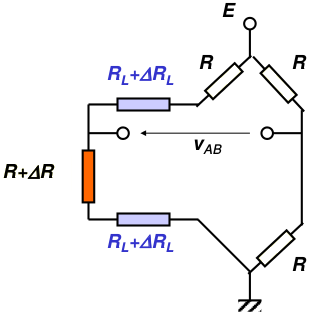
\includegraphics[scale=0.25]{ch2/image10.png}
\captionof{figure}{ }
\end{center}
Par simplification, 
on ne va s'arranger pour qu'elles soient négligeables. Pour se faire, analysons le spectre. 
La fonction sinus cardinal a un lobe principal : toute l'énergie est proche de l'origine. Nous 
allons travailler de sorte que les objets diffractant vérifient
\begin{equation}
\dfrac{2\pi}{l} \ll k = \dfrac{2\pi}{k}
\end{equation}
A ce moment la, le spectre est fort ramené à l'origine de sorte à ce que les ondes évanescentes 
soient négligées. Autrement dit
\begin{equation}
\int_{|\rho|>l} |A(\rho)|^2\ d\rho \ll \int_{-k}^{+k} |A(\rho)|^2\ d\rho
\end{equation}
Ce qui exprime que le spectre soit centrée sur l'origine et très étroit. Il faut dès lors que 
les objets diffractant sont significativement plus grand que la longueur d'onde : $\lambda \ll l$.\\

Le calcul de l'intégrale n'est pas évident (le facteur de phase gène). Nous allons utiliser 
l'approximation faite pour les ondes évanescentes :
\begin{equation}
\rho \approx \dfrac{2\pi}{l} \ll k
\end{equation}
On va pouvoir approximer le propagateur permettant de  ce cas, mais ceci est l'objet de la 
suivante section.
\end{enumerate}

\newpage
\section{Formule de diffraction de Fresnel}
Nous nous attarderons ici à reconstruire la fameuse formule de diffraction proposée par 
Fresnel sans se baser sur la transformée de Fourier (juste naissant) et les équations 
de Mawell (n'existant pas encore). Cependant, dans le cadre de ce cours, nous utiliserons 
ces deux outils.\\

Repartons de l'approximation de la solution générale des équations de Maxwell (on retrouve 
bien la contrainte sur les modes de Fourier)
\begin{equation}
a(x,y;z) = \iint_{-\infty}^\infty A(\rho,\sigma)e^{i\rho x}e^{i\sigma y} e^{i\sqrt{k^2-\rho^2-
\sigma^2}z}\ d\rho d\sigma
\end{equation}

\begin{wrapfigure}[8]{l}{9.5cm}
\vspace{-4mm}
\includegraphics[scale=0.4]{ch2/image11.png}
\captionof{figure}{ }
\end{wrapfigure}
Nous allons ici approcher l'expression du propagateur. Une onde plane arrivée sur un écran 
percé. Chacune de ces ondes possédant un certain poids ($A$) se propage avec un certain 
angle ($\rho$ par rapport à $x$ et $\sigma$ par rapport à $y$). Nous travaillons dans la 
limite $\lambda \ll l$ pour négliger les ondes évanescentes de sorte à ce que les seules 
valeurs significatives\footnote{La pondération, c'est-à-dire l'amplitude $A$, n'est 
significative que pour les valeurs de $\rho$ proche de l'origine : $\rho,\sigma \ll k$} de 
$\rho$ soient incluent dans $\left[\frac{-\pi}{l};\frac{\pi}{l}\right]$.\\

\danger Le spectre limite les valeurs de $\rho$ et $\sigma$, ne pas confondre avec les 
(grandes) bornes d'intégration : le spectre sera bien toujours étroit et donc notre 
fonction est large.\\

Intéressons-nous à l'\textit{approximation paraxiale} : petits angles $\rho,\sigma\ll k$. 
En effet, lorsque $\rho,\sigma\ll k$ on travaille avec un arcsinus très faible, d'où le 
\textit{petits angles}. Ceci va permettre d'éliminer la racine, bien gênante dans notre 
S.G.
\begin{equation}
\beta = \sqrt{l^2-\rho^2-\sigma^2} = k\sqrt{1-\dfrac{\rho^2}{k^2}-\dfrac{\sigma^2}{k^2}}
\end{equation}
On peut dès lors utiliser l'approximation de McLaurin $\sqrt{1+\epsilon} \approx 1+\frac{1
}{2}\epsilon$ :
\begin{equation}
\beta \approx k\left[1-\dfrac{1}{2}\frac{\rho^2}{k^2}-\dfrac{1}{2}\dfrac{\sigma^2}{k^2}\right] =
k-\dfrac{1}{2}\dfrac{\rho^2}{k}-\dfrac{1}{2}\dfrac{\sigma^2}{k}\qquad\qquad\beta \in\mathbb{R}
\ \forall (\rho,\sigma)
\end{equation}
\begin{wrapfigure}[8]{r}{4cm}
\vspace{-4mm}
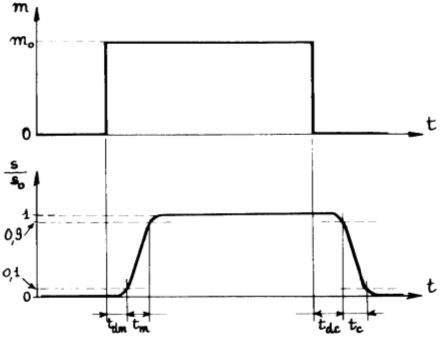
\includegraphics[scale=0.4]{ch2/image12.png}
\captionof{figure}{ }
\end{wrapfigure}
Le $\beta$ (la composante en $z$ du vecteur d'onde) obtenu est toujours réelle : la possibilité 
d'avoir des ondes évanescentes à été éliminée. Nous avons donc remplacé la contrainte sur 
les modes de Fourier (le vecteur d'onde devant se déplacer sur une sphère) a été changée en 
une contrainte de type parabolique. Ceci n'est valable que si la distribution angulaire est 
limitée ce qui n'est vrai que si la taille de l'objet est significativement grande devant la 
longueur d'onde.\\
Effectuons cette approximation par substitution :
\begin{equation}
a(x,y;z) = \iint_{-\infty}^\infty A(\rho,\sigma)e^{i\rho x}e^{i\sigma y} e^{i\frac{\rho^2}{2k}z
-i\frac{\sigma^2}{2k}z}\ d\rho d\sigma\ e^{ikz}
\end{equation}
Ceci est une simplification considérable, il va être possible de traiter ce terme de phase. Il 
suffit pour cela de remarquer que cette intégrale n'est que la transformée de Fourier inverse 
du spectre initial multiplié par le propagateur
\begin{equation}
a(x,y;z) = TF^{-1}\left[A(\rho,\sigma)e^{-i\frac{z}{2k}(\rho^2+\sigma^2)}\right]e^{ikz}
\end{equation}
Le facteur de phase étant quadratique, il est traitable analytiquement. Simplifions le problème 
en considérant que rien ne se passe en $y$ (le spectre est une delta de Dirac en $\sigma$) :
\begin{equation}
a(x;z) = TF^{-1}\left[A(\rho)\underbrace{e^{-\frac{z}{2k}\rho^2}}_{H_z(\rho)}\right]e^{ikz}
\end{equation}
On peut considérer que notre plaque percée obéit à la fonction fenêtre, suffisamment large devant 
la longueur d'onde\footnote{$z$ est un paramètre dans cette analyse.}. Plus proprement :
\begin{equation}
a(x;z) = TF^{-1}[A(\rho)H_z(\rho)]e^{ikz}
\end{equation}
Cette écriture nous permet d'utiliser le théorème de convolution de Fourier
\begin{equation}
a(x;z) = TF^{-1}[A(\rho)]\otimes TF^{-1}[H_z(\rho)]\ e^{ikz}
\end{equation}
Ou encore
\begin{equation}
a(x;z) = a(x;0)\otimes h_z(x)\ e^{ikz}
\end{equation}
où $a(x;0)$ est le champ initial, à l'endroit du plan diffractant. Avec la transformée de 
Fourier inverse (pour le peu que l'on intègre sur $\rho$) :
\begin{equation}
h_z(x) = \int e^{-i\frac{z}{2k}\rho^2}\ e^{i\rho x}\ d\rho
\end{equation}
Les tables mathématiques peuvent directement nous donner la solution de cette intégrale
\begin{equation}
h_z(x) = \sqrt{\frac{2k}{z}}\ e^{-i\dfrac{\pi}{4}}\ e^{i\dfrac{k}{2z}x^2}
\end{equation}
Ceci étant fait, explicitons la convolution à effectuer
\begin{equation}
a(x;z) = \int a(x':0)h_z(x-x')\ dx'\ e^{ikz}
\end{equation}
Après substitution
\begin{equation}
a(x;z) = \sqrt{\frac{2k}{z}}\int a(x';0) \ e^{-i\dfrac{\pi}{4}}\ e^{i\dfrac{k}{2z}(x-x')^2}\ 
dx'
\end{equation}
Il est aisé d'en dériver le résultat à deux dimensions transverses
\begin{equation}
h_z(x,y) = \sqrt{\frac{2k}{z}}\ e^{-i\dfrac{\pi}{4}}\ e^{i\dfrac{k}{2z}x^2} \times 
\sqrt{\frac{2k}{z}}\ e^{-i\dfrac{\pi}{4}}\ e^{i\dfrac{k}{2z}y^2}
\end{equation}
Après substitution
\begin{equation}
a(x,y;z) = \frac{2k}{z}\int a(x',y';0)\ e^{i\dfrac{k}{2z}(x-x)^2}\
 e^{i\dfrac{k}{2z}(y-y')^2}\ dx'dy'\ e^{-i\dfrac{\pi}{2}}\ e^{ikz}
\end{equation}
Ne faisant ici que du qualitatif, nous pouvons nous débarrasser des constantes. Intéressons
nous à cette fonction dont nous effectuons la convolution en incluant cette fois-ci le facteur 
de phase (la convolution ne portant que sur $x,y$ cela ne change rien)
\begin{equation}
a(x,y;z) = a(x,y:z)\otimes\left(h_z(x,y)\ e^{ikz}\right)
\end{equation}
où l'on s'intéresse à 
\begin{equation}
h_z(x,y)\ e^{ikz} = \frac{k}{z}\ e^{i\dfrac{k}{2z}(x^2+y^2)}\ e^{ikz}
\end{equation}
Qu'est ce que cette fonction? Nous savons qu'il s'agit de la fonction permettant de décrire 
le champ diffracté. C'est intéressant, mais qu'est ce qui permet de faire ça? Analysons la 
phase (quadratique, voir même parabolique) de ce terme
\begin{equation}
\varphi = \dfrac{k}{2z}x^2+\dfrac{k}{2z}y^2+kz
\end{equation}
Analysons la répartition de champ d'une onde sphérique $\frac{1}{r}e^{ikr}$ décrite en $kr$ 
où $k$ est un \textbf{nombre} d'onde (et pas un vecteur). On s'intéresse ici à la phase de 
cette onde : exprimons les lieux de phases constantes ou, autrement dit, les fronts d'ondes
\begin{equation}
\varphi = kr = 2m\pi
\end{equation}

\begin{wrapfigure}[8]{r}{4cm}
\vspace{-4mm}
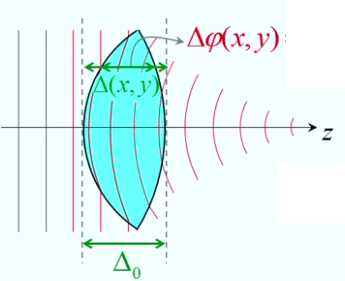
\includegraphics[scale=0.4]{ch2/image13.png}
\captionof{figure}{ }
\end{wrapfigure}
où $r = \sqrt{x^2+y^2+z^2}$. En se plaçant dans des conditions paraxiales (très proche de 
l'axe $z$) : $x,y \ll z$. On se propose donc d'analyser la phase d'une onde sphérique dans 
la zone ou les conditions paraxiales sont réunies. On peut approximer la racine
\begin{equation}
r\sqrt{1+\dfrac{x^2}{z^2}+\dfrac{y^2}{z^2}} \quad \Rightarrow \quad\left[1+\dfrac{x^2}{2z^2}+
\dfrac{y^2}{2z^2}\right]
\end{equation}
Dès lors
\begin{equation}
\varphi = kr = kz+ \dfrac{k}{2z}x^2+\dfrac{k}{2z}y^2 = 2m\pi
\end{equation}
Il s'agit d'un paraboloïde, c'est bien une approximation parabolique de fronts d'onde 
sphériques, généralement générés par des petites sources ponctuelles d'ondes électromagnétiques 
assimilables à des delta de Dirac, le champ magnétique vibre en un point de l'espace et 
génère une onde sphérique.\\

\begin{wrapfigure}[11]{l}{3.5cm}
\vspace{-5mm}
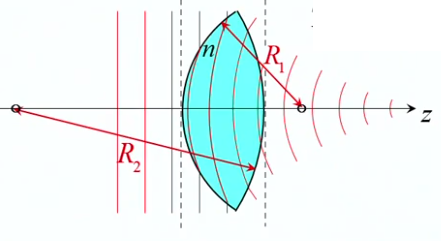
\includegraphics[scale=0.4]{ch2/image14.png}
\captionof{figure}{ }
\end{wrapfigure}
Revenons à notre problème. Le champ initial est la fameuse fonction fenêtre. Après une certaine 
distance parcourue, on récupère un certain profil donne par (ici) un profil à deux dimensions. 
Nous pouvons voir ça comme un système linéaire (en effet, des ondes rentrent et en sortent 
modifiées). Nous avions déjà rencontré ce système en  utilisant le principe de superposition, 
les équations de Maxwell étant linéaires dans le vide\footnote{On peut voir toute onde comme 
une combili d'ondes harmoniques}. \\

Le champ est un produit de convolution du champ d'entrée avec une fonction de phase quadratique qui 
ne représente rien d'autre qu'une phase sphérique. Nous voyons une sommes d'ondes sphériques en 
approximation paraboliques mis sous la forme d'une convolution. En effet, le $x-x'$ représente le 
fait que l'onde ne vient plus de l'origine (comme dans $h_z$) mais désigne un point qui n'est plus 
à l'origine mais au point $(x',y')$.
\begin{equation}
r = \sqrt{(x-x')^2+z^2}
\end{equation}
En approchant ceci par l'approximation parabolique
\begin{equation}
r \approx z+\dfrac{(x-x')^2}{2z}
\end{equation}
Ceci est précisément ce qui apparaît dans notre convolution\footnote{Débarrassée des constantes.} :
\begin{equation}
a(x,y;z) = \frac{k}{z}\int a(x',y';0)\ e^{i\dfrac{k}{2z}(x-x)^2}\
 e^{i\dfrac{k}{2z}(y-y')^2}\ dx'dy'\  e^{ikz}
\end{equation}

Nous ne travaillons finalement que avec la "\textit{réponse impulsionnelle}" du système où 
l'impulsion est cette source ponctuelle située en $(x',y')$. Nous avons en effet la réponse 
à une source ponctuelle (un delta, cette fois ci non temporel mais spatial) générant l'onde 
$h_z$ (l'onde sphérique approchée de façon parabolique) $\rightarrow$ réponse impulsionnelle.\\


Un point source donne lieu à une certaine répartition de champ. La réponse globale s'obtient en 
prenant la convolution avec cette réponse, c'est-à-dire en considérant que chaque point a une 
certaine amplitude $a(x',y';0)$ : l'objet à une certaine amplitude et chaque de ces amplitude 
rayonne une onde sphérique partant de $(x',y')$ ou l'on a une certaine amplitude. \\

\begin{wrapfigure}[9]{l}{6.5cm}
\vspace{-5mm}
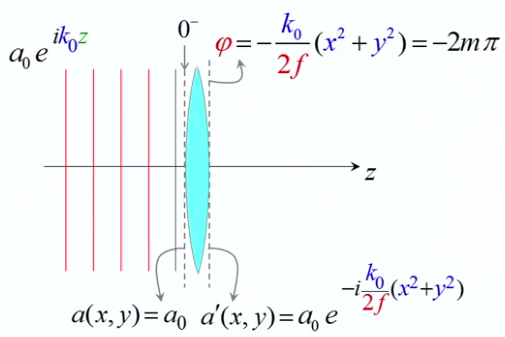
\includegraphics[scale=0.4]{ch2/image15.png}
\captionof{figure}{ }
\end{wrapfigure}
On retrouve le 
principe de Huygens : un écran laisse passé un trou laissant passé la lumière avec une certaine 
amplitude dépendant de $x'$ et $y'$. Chaque point de cet objet peut être considéré comme un point 
source générant une onde sphérique pouvant être approchée paraboliquement. En $z$, nous sommons 
(à travers l'intégrale) les champs de chacune de ces ondes sphériques. Nous avons une 
superposition d'onde sphérique d'amplitude donnée par l'amplitude de l'objet de départ : la 
figure de diffraction résultera des interférences entre toutes ces ondes sphériques (seulement une 
est représentée ci-contre).\\

Ceci est ainsi de la formule de diffraction de Fresnel, cette intégrale de Fresnel ne représente 
rien d'autre qu'une superposition d'ondelettes de Huygens.
\begin{equation}
a(x,y;z) = \frac{2k}{z}\int a(x',y';0)\ e^{i\dfrac{k}{2z}(x-x)^2}\
 e^{i\dfrac{k}{2z}(y-y')^2}\ dx'dy'\ e^{-i\dfrac{\pi}{2}}\ e^{ikz}
\end{equation}


Analysons les amplitudes des ondelettes de Huygens, ici en analysant leur amplitude. Considérons 
une de ces ondes, celle venant de l'origine ($x'=y'=0$) :
\begin{equation}
a(x,y;z) = \dfrac{k}{z}e^{i\dfrac{k}{2z}(x^2+y^2)}\ e^{ikz}
\end{equation}
Il s'agit de la fonction $h_z$ que nous avions précédemment\footnote{Pq?}



Nous avons une onde sphérique approchée par une onde parabolique dont le profil d'intensité 
(le module carré du champ) est donné par
\begin{equation}
I(x,y;z) = |a(x,y;z)|^2 \propto \dfrac{1}{z^2}
\end{equation}
Ceci peut paraître curieux car la décroissance réelle d'une onde est en $\frac{1}{r^2}$.
\begin{equation}
I(x,y;z) \propto \frac{1}{r^2}
\end{equation}
Pourquoi donc ? Il ne faut pas oublier que la notion d'intensité est locale : c'est la 
densité de flux énergétique de l'onde ($W/m^2$). S'il y a une certaine radiation la puissance 
totale s'obtient par l'intégration de cette radiation sur une sphère : on obtient la 
puissance radiée par la source (on obtient de $W$). La puissance rayonnée au travers de cette 
sphère est donnée par $4\pi r^2 I$ où $r$ est le rayon de la sphère sur laquelle on intègre. 
Or, cette intensité doit bien être constante (indépendante de $r$) : peu importe la sphère, 
la puissance émise de la source est constante, d'où la variation en $r^{-2}$.\\

\begin{wrapfigure}[9]{r}{5cm}
\vspace{-5mm}
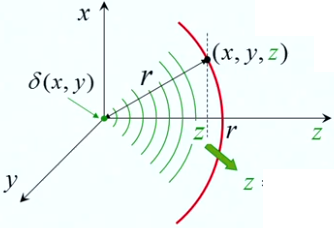
\includegraphics[scale=0.4]{ch2/image16.png}
\captionof{figure}{ }
\end{wrapfigure}
Or, nous obtenons $1/z^2$ et non pas $1/r^2$. Analysons pour cela l'onde sphérique en un 
point de coordonnée $(x,y,z)$ correspondant à un certain rayon : il y a une différence 
entre $z$ et $r$ (voir schéma ci-contre). Faisons la comparaison. Considérons $r$ dans le 
cadre de l'approximation paraxiale $x,y \ll z$ :
\begin{equation}
r = z+\frac{1}{2z}(x^2+y^2) + \mathcal{O}(2)
\end{equation}



En réalité, pour décrire cette onde, le front d'onde en $e^{ikz}$ a été approché : la 
sphère a été approché par une parabole, l'ordre un du développement a été gardé. Or, nous 
sommes passé de $1/r$ à $1/z$ car nous n'avons pas fait la même 
approximation. Pour la phase on considère que $r = z +\frac{1}{2z}(x^2+y^2)$ et pour l'amplitude 
on dit que $r=z$ (l'ordre un pour l'amplitude a été supprimé). Ceci peut paraître paradoxal, 
mais c'est parce que nous avons considéré 
\begin{equation}
\frac{1}{z^2}\approx\frac{1}{r^2}
\end{equation}
On peut se permettre de faire ça car une petite erreur sur la phase peut résulter en de 
grandes erreurs du profil diffracté. Mais si on se trompe sur la valeur de $r$ (petite 
erreur : $\delta r \approx 10^{-6}m\approx \lambda$) peut créer une erreur sur la phase 
de l'ordre de 100\% alors que sur l'amplitude, cela ne change quasiment rien. Il est donc 
tout à fait légitime de garder l'approximation d'ordre 1 pour évaluer la distance dans le 
terme de phase et de se contenter de l'approximation d'ordre 0 pour l'amplitude.



\newpage
\section{Formule de diffraction de Fraunhofer}
Pour établir cette nouvelle formule, repartons de la formule de diffraction de Fresnel
\begin{equation}
a(x,y;z) = \frac{k}{z}\int a(x',y';0)\ e^{i\dfrac{k}{2z}(x-x)^2}\
 e^{i\dfrac{k}{2z}(y-y')^2}\ dx'dy'\  e^{ikz}
\end{equation}
Rappelons l'interprétation physique de cette formule.
A partir de la connaissance du champ électromagnétique lumineux dans un certain plan 
($z=0$) on peut connaître le champ en toute position $z$ grâce à cette formule. Dans 
celle-ci nous retrouvons la phase des ondelettes de Huygens. Ce phaseur d'ondelette 
est multiplié par une amplitude puis on sommera tout via les intégrales. Intéressons-
nous à la phase de ces ondelettes où les carrés ont été développés
\begin{equation}
\varphi = kz + \frac{k}{2z}\left[x^2 + y^2 + x^{'2} + y^{'2} - 2xx'-2yy'\right]
\end{equation}
La diffraction de Fraunhofer fait un pas supplémentaire dans l'approximation de ces 
ondelettes : on va négliger les termes\footnote{Les axes en prim' sont ceux du repère 
attaché à l'objet diffractant.} $x^{'2}$ et $y^{'2}$ (mais on les garde au premier 
ordre). Pour se faire, nous allons limiter la taille de l'objet
\begin{equation}
x',y' \ll x,y
\end{equation}
En réalité, c'est la phase $\frac{kx^{'2}}{2z}$ que l'on choisi de négliger, c'est-à-dire
\begin{equation}
e^{i\dfrac{k}{2z}\|\vec{x'}\|^2_{\max}} \approx 1\qquad\Rightarrow\qquad \dfrac{k}{2z}\|
\vec{x'}\|^2_{\max}\ll 1
\end{equation}
où $\|\vec{x'}\|^2_{\max}$ est la plus grande distance depuis l'origine à l'extrémité 
de l'objet. Si ce facteur de phase est proche de l'unité, ce terme en prim' carré peut 
bien être supprimé. On peut écrire
\begin{equation}
\dfrac{k}{2}\|\vec{x'}\|^2_{\max} \ll z
\end{equation}
Or $k = \frac{2\pi}{\lambda}$, dès lors
\begin{equation}
\dfrac{\pi}{\lambda}\|\vec{x'}\|^2_{\max} \ll z
\end{equation}

\begin{wrapfigure}[9]{r}{7.5cm}
\vspace{-5mm}
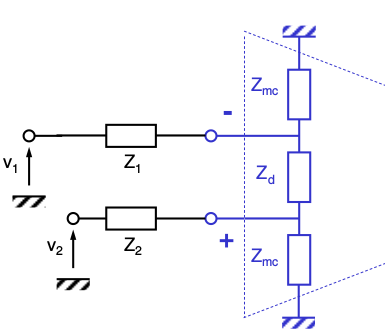
\includegraphics[scale=0.45]{ch2/image17.png}
\captionof{figure}{ }
\end{wrapfigure}
Si la distance $z$ est plus grande que la taille de l'objet au carré divisée par la longueur 
d'onde (le facteur pi ne change pas l'ordre de grandeur), cette approximation est bien valide
et on  parlera de \textit{zone de Fraunhofer}. Il ne reste que des termes linéaires dans notre 
phase
\begin{equation}
\varphi = kz + \frac{k}{2z}\left[x^2 + y^2 - 2xx'-2yy'\right]
\end{equation}
Après substitution
\begin{equation}
a(x,y:z) = \frac{k}{z}\int a(x',y';0) e^{i\frac{k}{2}(x^2+y^2)}e^{-i\frac{k}{z}(xx'+yy')}\ 
dx'dy'\ e^{ikz}
\end{equation}
En regroupant les termes de phases, on peut écrire
\begin{equation}
a(x,y:z)e^{ikz} e^{i\frac{k}{2}(x^2+y^2)} = \frac{k}{z}\int a(x',y';0) e^{-i\frac{k}{z}(xx'+yy')}\ 
dx'dy'\ 
\end{equation}
En séparant le terme de phase en deux
\begin{equation}
a(x,y:z) = \dfrac{k}{z} e^{ikz} e^{i\dfrac{k}{2}(x^2+y^2)} \underbrace{\int a(x',y';0) e^{-i\dfrac{k
}{z}xx'}e^{-i\dfrac{k}{z}yy'}\ dx'dy'}_{A\left(\frac{kx}{z},\frac{ky}{z}\right)}
\end{equation}
En posant $\rho = k/zx$ et $\sigma = k/zy$ on retrouve la définition de la transformée de Fourier 
$A(\rho,\sigma)$ : il s'agit de la transformée de Fourier du champ objet. Dès lors\\

\retenir{\textbf{Formule de diffraction de Fraunhofer}
\begin{equation}
a(x,y;z) = \dfrac{k}{z} e^{ikz} e^{i\dfrac{k}{2}(x^2+y^2)}\ A\left(\frac{kx}{z},\frac{ky}{z}\right)
\end{equation}
où $A$ est la transformée de Fourier du champ objet en $z=0$.}\ 

Ce qui n'est rien d'autre qu'un facteur de phase multiplié par un certain spectre aux variables 
un peu plus particulière que d'habitude. Le profil d'intensité sera ainsi directement 
proportionnel à la densité spectrale
\begin{equation}
I(x,y) \propto \left| \left(\frac{kx}{z},\frac{ky}{z}\right) \right|^2
\end{equation}

\begin{wrapfigure}[10]{l}{7cm}
\vspace{-5mm}
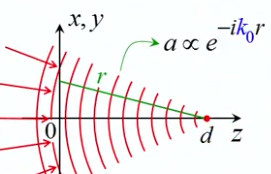
\includegraphics[scale=0.45]{ch2/image18.png}
\captionof{figure}{ }
\end{wrapfigure}
Intéressons-nous à l'interprétation physique de cette formule. Plutôt que de considérer le 
problème tridimensionnel des ondelettes de Huygens, revenons à un cas plus simple (une 
dimension transverse $x'$. Commençons par interpréter le premier facteur. Considérons 
"l'ondelette centrale" c'est-à-dire celle donnée par la formule de Fresnel en $x'=y'=0$ : 
dans ce cas, la phase est identique à celle présente dans le terme de hase de la 
formule de diffraction de Fraunhofer. On reconnaît donc l'ondelette de Huygens pour un 
point centré à l'origine. Ceci est normal, car à grande distance les deux sources 
ponctuelles ne semblent former qu'une de sorte à ce qu'à grande distance, les fronts d'
ondes soient superposés. La répartition de phase est très proche de celle de l'ondelette 
d'Huygens centrée à l'origine, avec le fameux décroissement en $1/z^2$.\\


\begin{wrapfigure}[10]{r}{7cm}
\vspace{-3mm}
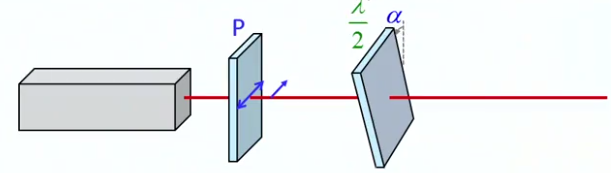
\includegraphics[scale=0.45]{ch2/image19.png}
\captionof{figure}{ }
\end{wrapfigure}
Le second terme, la modulation d'amplitude, est plus délicat à interpréter. Pour se faire, 
repartons du point de départ de l'établissement de la formule de diffraction de Fresnel :
\begin{equation}
a(x,y;z) = \iint_{-\infty}^\infty A(\rho,\sigma)e^{i\rho x}e^{i\sigma y} e^{i\sqrt{k^2-\rho^2-
\sigma^2}z}\ d\rho d\sigma
\end{equation}
Ce qui n'est rien d'autre que la S.G. de Maxwell. Passons à une dimension transverse (une 
delta pour le $\sigma$) $x'$ :
\begin{equation}
a(x;z) = \int A(\rho)e^{i\rho x} e^{i\sqrt{k^2-\rho^2}z}\ d\rho 
\end{equation}
De même, le résultat de Fraunhofer devient
\begin{equation}
I(x) \propto \left|A\left(\dfrac{kx}{z}\right)\right|^2
\end{equation}
Dans Fresnel, $A(\rho)$ est le spectre en $z=0$, chaque valeur de $\rho$ représentant une 
onde plane avec un certain angle ($\rho = k\sin\theta$, soit la projection en $x$ du 
vecteur d'onde)(comme nous travaillons à petit angle : $\rho = k\theta$). L'intensité à une 
certaine hauteur $x$ vient d'une onde possédant un certain angle $\theta$. On en tire
\begin{equation}
\tan \theta = \dfrac{x}{z}\qquad \rightarrow \qquad \rho = k\frac{x}{z}
\end{equation}

\begin{wrapfigure}[10]{l}{6.5cm}
\vspace{-3mm}
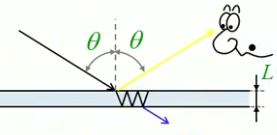
\includegraphics[scale=0.45]{ch2/image20.png}
\captionof{figure}{ }
\end{wrapfigure}
On sélectionne ainsi l'onde plane ayant pour valeur de $\rho = kx/z$. On comprend maintenant 
bien pourquoi on observe ce $A(kx/z)$. Hélas, sur notre schéma ci-dessous les ondes planes 
sont dessinées "limitées". Or, en réalité, elles ont bien une extension infinie ce qui rend 
l'interprétation physique bien moins satisfaisante. Du moins, c'est ce que l'on pourrait 
croire (que l'onde plane éclaire tout le plan) mais c'est faux (ouf!). Comment le justifier 
? Pourquoi n'éclaire-t-elle qu'un seul point ? Il faut aller plus loin dans l'interprétation. 
Pour se faire, il est nécessaire d'utiliser le \textit{théorème des phases stationnaires}.

	\subsection{Théorème des phases stationnaires}
	Nous allons appliquer ce théorème au calcul de l'intégrale de Fourier suivante
	\begin{equation}
	a(x;z) = \int A(\rho)\ e^{i\rho x}e^{i\sqrt{k^2-\rho^2}z}\ d\rho
	\end{equation}
	sur laquelle nous appliquer l'approximation paraxiale
	\begin{equation}
	\sqrt{k^2-\rho^2} = k-\frac{1}{2}\frac{\rho^2}{k}
	\end{equation}
	Après substitution
	\begin{equation}
	a(x;z) = \int A(\rho)\ e^{i\rho x}e^{-i\frac{z}{2k} z}\ d\rho\ e^{ikz}
	\end{equation}
	Intéressons-nous à la phase de cette intégrande 
	\begin{equation}
	\varphi(\rho) = \rho x - \dfrac{z}{2k}\rho^2
	\end{equation}
	
	\begin{wrapfigure}[15]{r}{4.5cm}
	\vspace{-3mm}
	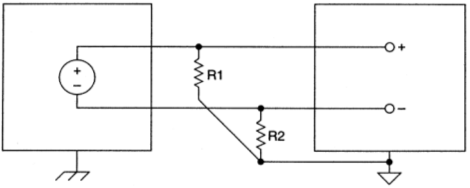
\includegraphics[scale=0.5]{ch2/image21.png}
	\captionof{figure}{ }
	\end{wrapfigure}
	Il s'agit d'une parabole, la dépendance de $\varphi$ en $\rho$ présente bien un 
	maximum. Regardons le phaseur (l'exponentielle de $i\varphi$). Représentons la 
	partie réelle de cette exponentielle (par facilité, mais n'oublions pas qu'il 
	existe une partie imaginaire). Au moment du maximum, $\varphi$ ne varie que peu 
	et l'on observe un état "stationnaire" du cosinus. Lorsque $\varphi$ varie 
	rapidement, on observe bien des oscillations rapide du cosinus. Comme nous avons 
	considéré un objet petit, le spectre sera forcément large. Or, nous avons le 
	produit du spectre par l'exponentielle imaginaire représentée par le cosinus. Dans 
	les zones de variation rapide, le produit sera approximativement nul, la seule 
	partie ayant une contribution notable est celle correspondant à une variation 
	lente du cosinus, donnant quelque chose de proportionnel au spectre (le cosinus 
	valant $\approx 1$). On nomme ci-contre $\rho^*$ la valeur pour laquelle nous 
	avons la stationarité de la phase, c'est-à-dire
	\begin{equation}
	\varphi'(\rho^*)=0\quad \Leftrightarrow\quad \rho^* = \dfrac{kx}{z}
	\end{equation}
	\newpage
	
		\begin{wrapfigure}[15]{l}{4.5cm}
%	\vspace{-3mm}
	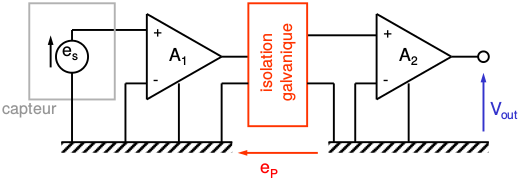
\includegraphics[scale=0.5]{ch2/image22.png}
	\captionof{figure}{ }
	\end{wrapfigure}
	On retrouve le résultat de Fraunhofer, $a(x;z) \propto A\left(\dfrac{kx}{z}
	\right)$. Il faut maintenant vérifier que nous sommes dans les conditions de 
	notre approximation. Considérons la phase stationnaire et descendons de $\pi$ (car 
	au déla, les oscillations sont rapides, le résultat du produit est nul). Ceci 
	correspond à une largeur $\delta \rho$ (la largeur de la fonction cosinus). Or, 
	il est possible d'évaluer ce $\delta\rho$ car nous avons connaissance de l'expression 
	de notre parabole
	\begin{equation}
	\dfrac{z}{2k}\delta\rho^2 = \pi\quad\Leftrightarrow\quad \delta\rho^2 = \dfrac{
	2\pi k}{z}
	\end{equation}
	Pour que le théorème des phases soit variable, il faut que le $\delta \rho$ soit 
	beaucoup plus petite que la variation du spectre (on considère que le spectre 
	est constant sur $\Delta \rho$ (extension spectrale suffisamment grande)
	\begin{equation}
	\delta\rho^2 = \dfrac{2\pi k}{z} \ll \Delta \rho^2
	\end{equation}
	Or, la largeur spectrale de notre fonction fenêtre vaut $2\pi/l$, on peut dire que 
	$\Delta \rho \approx \frac{2\pi}{\|\vec{x'}\|_{\max}}$. Dès lors
	\begin{equation}
	\dfrac{2\pi k}{z}\ll \dfrac{4\pi^2}{\|\vec{x'}\|_{\max}^2}
	\end{equation}
	En explicitant $k=2\pi/\lambda$, en simplifiant : $\frac{\|\vec{x'}\|^2_{\max}}{\lambda}
	\ll z$ ce qui est la zone de Fraunhofer ! Ce théorème est donc applicable.\\
	

\begin{wrapfigure}[10]{l}{6.5cm}
	\vspace{-3mm}
	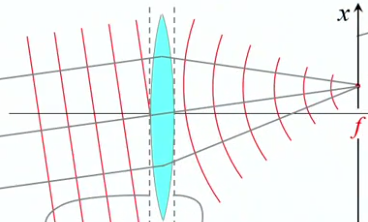
\includegraphics[scale=0.45]{ch2/image23.png}
	\captionof{figure}{ }
	\end{wrapfigure}	
Le théorème des phases stationnaires nous dit que si l'on observe $A\left(\dfrac{kx}{z}
\right)$ à un seul point (et non pas tout l'écran) c'est parce que en ce point la il va 
y avoir interférences constructives entre les ondes. Représentons une onde plane qui a une 
valeur de $\rho$ légèrement supérieure. Ces ondes ont des interférences constructives au 
point considéré et quelconques ailleurs : toutes les zones au $\rho$ proche vont 
construire un champ important au point $x$. Aux autre points, on sommes des champs aléatoires 
pour obtenir finalement zéro. C'est ce que dit notre théorème, nous n'avons interférences 
constructives que proche de $\rho \approx \rho^*$, le reste ne contribue pas.
	







































\chapter{Représentations position - impulsion}
Commençons par rappeler quelques notions dans la base position
\begin{equation}
\ket{\psi} = \int d\vec r\ \psi(\vec{r})\ket{\vec{r}}
\end{equation}
où les coefficients de Fourier sont donnés par $\psi(\vec{r}) = \bra{\vec{r}}\ket{\psi}$.
\begin{equation}
\bra{\psi}\ket{\psi} = \iint d\vec r\ d\vec r'\psi^*(\vec{r'})\psi(\vec{r})\underbrace{
\bra{\vec{r'}}\ket{\vec{r}}}_{\delta(\vec{r},\vec{r'})} = \int d\vec r |\psi(\vec{r}|^2=1
\end{equation}
Avec la décomposition spectrale $\hat{\vec{r}} = \int d\vec{r}\ \vec{r}\ket{\vec{r}}\bra{\vec{r}}$, 
on peut écrire\footnote{Si tu veux je peux détailler le raisonnement pour la valeur moyenne...}
\begin{equation}
\mathbb{P}(\vec{r}) = \underbrace{\bra{\psi}\ket{\vec{r}}}_{\psi^*(\vec{r})}\underbrace{
\bra{\vec{r}}\ket{\psi}}_{\psi(\vec{r})} = |\psi(\vec{r})|^2,\qquad\qquad\langle\hat{\vec{r}}\rangle = 
\bra{\psi}\hat{\vec{r}}\ket{\psi} = \int d\vec{r}\ \vec{r}\underbrace{\bra{\psi}\ket{\vec{r}}
\bra{\vec{r}}\ket{\psi}}_{|\psi(\vec{r})|^2}
\end{equation}

\section{Opérateur impulsion}
Pour motiver physiquement l'opérateur impulsion, repartons de la notion d'onde de de Broglie que 
l'on peut associer à une particule libre ayant une certaine vitesse. 
\subsection{Onde de De Broglie, paquets d'onde}
		\subsubsection{Onde de De Broglie}
		Grâce à de Broglie, on associe une onde à toute particule en mouvement.
		Par analogie avec les concepts de l'électromagnétisme, décrivons cette onde au moyen d'exponentielles complexes.
		%On peut voir une particule comme une onde, de Broglie a réussi à donner les "paramètres" de cette onde.
		% Voyons ça comme une onde, par analogie à l'électromagnétisme
		\begin{equation}
		\psi(\vec{r},t) = \psi_0e^{i(\vec{k}\vec{r}-\omega t)}
		\end{equation}
		De Broglie pose les valeurs qu'il faut associer à $\vec k$ et $\omega$ pour une particule ayant 
		une certaine vitesse et énergie. Le point de départ est
		\begin{equation}
		\lambda = \dfrac{h}{p},\qquad k=\dfrac{2\pi}{\lambda},\qquad \vec k=\dfrac{\vec{p}}{\hbar}
		\end{equation}
		Pour la fréquence, par analogie à l'optique\footnote{As-tu vérifié la chronologie ?}
		\begin{equation}
		\nu = \dfrac{E}{h},\qquad \omega = 2\pi\nu = \dfrac{E}{\hbar}
		\end{equation}
		En substituant ces expressions dans l'expression de l'onde plane
		\begin{equation}
		\psi(\vec{r},t) = \psi_0\ e^{\frac{i}{\hbar}\left(\vec{p}.\vec{r}-Et\right)}\qquad \text{ où }\ \psi_0 =
		\dfrac{1}{(2\pi\hbar)^{3/2}} \text{ pour la normalisation}
		\end{equation}
		Cette solution étant écrite par analogie avec l'EM, il est possible d'écrire une équation 
		d'onde que cette onde va vérifier. Regardons par exemple si l'on effectue
		\begin{equation}
		\begin{array}{lll}
		\bullet i\hbar\frac{\partial}{\partial t}\psi &= i\hbar \psi_0\frac{E}{i\hbar}e^{\dots} &=
		E\psi(\vec{r},t)\\
		\bullet \Delta \psi(\vec{r},t) &= \psi_0\dfrac{p_x^2+p_y^2+p_z^2}{(-i\hbar)^2}e^{\dots} &= -
		\dfrac{p^2}{\hbar^2}\psi(\vec{r},t)
		\end{array}
		\end{equation}
		On en tire pour une particule libre
		\begin{equation}
		-\dfrac{\hbar^2}{2m}\Delta \psi(\vec{r},t) = \dfrac{p^2}{2m}\psi(\vec{r},t) = E\psi(\vec{r},t)
		\end{equation}
		On retrouve le classique
		\begin{equation}
		\underline{i\hbar\dfrac{\partial}{\partial t}\psi(\vec{r},t)= -\dfrac{\hbar^2}{2m}\Delta\psi(\vec{r},t)}
		\end{equation}
		Il s'agit d'une ED de type d'onde qui est bien vérifiée par l'onde plane construite ci-dessus. 
		Cette ED correspond à une particule libre. Elle est linéaire : toute combili de solution est 
		solution. Au lieu de prendre une onde de de Broglie monocinétique correspondant à une onde 
		monochromatique, on peut considérer un paquet d'onde. Par exemple
		\begin{equation}
		\left.\begin{array}{ll}
		p_1 \rightarrow \psi_1\\
		p_2 \rightarrow \psi_2
		\end{array}\right\}\longrightarrow \alpha\psi_1+\beta\psi_2
		\end{equation}
		Un paquet d'onde est une superposition continue de particules avec toute une gamme de vitesse 
		possible. Il y correspondra une onde de de Broglie nommée \textit{paquet d'ondes}.

		\subsubsection{Paquet d'ondes}
		En substituant le préfacteur $\psi_0$, on obtient
		\begin{equation}
		\psi(\vec{r},t) = \dfrac{1}{(2\pi\hbar)^{3/2}}\int d\vec{p}\ \phi(\vec{p})e^{\frac{i}{\hbar}(\vec{p}
		\vec{r}-Et)}
		\end{equation}
		
	\subsection{Dualité des bases position et impulsion (transformée de Fourier)}
	La même expression, en notation de Dirac :
	\begin{equation}
	\ket{\psi} = \int d\vec{p}\ \phi(\vec{p})\ket{\vec{p}}
	\end{equation}
	Il s'agit d'un mélange (avec un certain poids) de kets $\bra{\vec{p}}$. En refermant
		\begin{equation}
	\psi(\vec{r},t) = \bra{\vec{r}}\ket{\psi} = \int d\vec{p}\ \phi(\vec{p})\underbrace{
	\bra{\vec{r}}\ket{\vec{p}}}_{(*)}
	\end{equation}
	où $\DS (*) = \frac{1}{(2\pi\hbar)^{3/2}}e^{\frac{i}{\hbar}(\vec{p}\vec{r}-Et)}$.
	Pour une raison d'élégance, intégrons le facteur de phase temporel dans un ket.	
%	 On voudrait 
%	faire la même chose mais en intégrant la phase dans le ket
	\begin{equation}
		\psi(\vec{r},t) = \frac{1}{(2\pi\hbar)^{3/2}}\int d\vec{p} \underbrace{\phi(\vec{p})e^{-\frac{i}
	{\hbar}Et}}_{\phi(\vec{p},t)}e^{\frac{i}{\hbar}\vec{p}.\vec{r}}
	\end{equation}
	\textbf{Attention} : ce n'est plus le même $\ket{\vec{p}}$ qu'à la précédente expression, la 
	définition à ici changée afin de pouvoir écrire
	\begin{equation}
	\ket{\psi} = \int d\vec{p}\ \phi(\vec{p},t)\ket{p}
		\end{equation}
	En refermant
	\begin{equation}
	\psi(\vec{r},t) = \bra{\vec{r}}\ket{\psi} = \int d\vec{p}\ \phi(\vec{p},t)
	\underbrace{\bra{\vec{r}}\ket{\vec{p}}}_{(**)}
		\end{equation}
	où $\DS (**)= \frac{1}{(2\pi\hbar)^{3/2}}e^{\frac{i}{\hbar}\vec{p}.\vec{r}}$ est le 
	\textbf{noyau de la transformée de Fourier}.\\
	
	Résumons
	\begin{equation}
		\ket{\psi}\left\{\begin{array}{ll}
	= \int d\vec{r}\ \psi(\vec{r},t)\ket{\vec{r}} & \rightarrow\text{Base pos.}\\
	= \int d\vec{p}\ \phi(\vec{p},t)\ket{\vec{p}} & \rightarrow\text{Base imp.}		
	\end{array}\right.
	\end{equation}
	avec
		\begin{equation}
	\underline{\bra{\vec{r}}\ket{\vec{p}} = \frac{1}{(2\pi\hbar)^{3/2}}e^{\frac{i}{\hbar}\vec{p}.\vec{r}}}
	\end{equation}
	Il s'agit de la \textit{formule de changement de base}. Elle est particulièrement intéressante :
	\begin{equation}
	\begin{array}{ll}
		\psi(\vec{r},t) = \bra{\vec{r}}\ket{\psi} &= \int d\vec{p}\ \phi(\vec{p},t)\ \bra{\vec{r}}\ket{\vec{p}}\\
	&= \frac{1}{(2\pi\hbar)^{3/2}}\int d\vec{p}\ \phi(\vec{p},t)e^{\frac{i}{\hbar}\vec{p}\vec{r}}\\
	\phi(\vec{p},t) = \bra{\vec{p}}\ket{\psi} &= \int d\vec{r}\ \psi(\vec{r},t)\ \bra{\vec{p}}\ket{\vec{r}}\\
	&= \frac{1}{(2\pi\hbar)^{3/2}}\int d\vec{r}\ \psi(\vec{r},t)e^{-\frac{i}{\hbar}\vec{p}\vec{r}}		
	\end{array}
		\end{equation}
	On remarque qu'il existe une transformée de Fourier qui lie les bases position et impulsion.
	On peut écrire
	\begin{equation}
	\underline{\phi(\vec p) = TF[\psi(\vec{r})]},\qquad\qquad \underline{\psi(\vec r) = TF^{-1}
	[\phi(\vec{p})]}
	\end{equation}
		
	
	Il en découle une série de propriétés
	\begin{itemize}
	\item[i.] \textit{Théorème de Parseval }: le produit scalaire de deux fonctions vaut le produit 
	scalaire des TF de ces deux fonctions. 
		\begin{equation}
	\int f_1(\vec{r})f_2^*(\vec{r}) d\vec{r} = \int F_1(\vec{p})F_2^*(\vec{p})d\vec{p}
	\end{equation}
	Dans notre cas :
	\begin{equation}
	\bra{\psi_1}\ket{\psi_2} \left\{\begin{array}{ll}
		= \int d\vec{r}\ \underbrace{\bra{\psi_1}\ket{\vec{r}}}_{\psi_1^*(\vec{r})}
	\underbrace{\bra{\vec{r}}\ket{\psi_2}}_{\psi_2(\vec{r})}\\
	= \int d\vec{p}\ \underbrace{\bra{\psi_1}\ket{\vec{p}}}_{\phi_1^*(\vec{p})}
	\underbrace{\bra{\vec{p}}\ket{\psi_2}}_{\phi_2(\vec{p})}		
	\end{array}\right.
	\end{equation}
		La normalisation est conservée par le changement de base
	\begin{equation}
	1 = \bra{\psi}\ket{\psi} = \int d\vec{r}\ |\psi(\vec{r})|^2 = \int d\vec{p}\ |\phi(\vec{p})|^2
	\end{equation}
	
	\item[ii.] \textit{Relation d'incertitude $\hat{x}-\hat{p}$}: on peut voir Robertson comme une 
	conséquence de ces TF : la TF d'une fonction étroite sera large et inversément. Il y a quelque chose qui peut
	 s'apparenter à une relation d'incertitude $\hat x-\hat p$. Nous avons
	 \begin{equation}
	 \langle p^2\rangle = \int |\phi(p)|^2\ p^2\ dp
	 \end{equation}
	Alors
	\begin{equation}
	\begin{array}{ll}
	\Delta p^2 &= \langle p^2 \rangle-\langle p\rangle^2 \longleftarrow |\phi(p)|^2\\
	\Delta x^2 &= \langle x^2 \rangle-\langle x\rangle^2 \longleftarrow |\psi(x)|^2
	\end{array}\Longrightarrow \Delta \hat x\Delta\hat{p} \geq\frac{\hbar}{2}
	\end{equation}
	Si on a une paire de fonctions (ici $\psi$ et $\phi$) qui sont "connectées" par une TF, dans la 
	théorie des TF le produit des variances peut être minoré par une constante. Cette démonstration
	ne sera pas faite ici mais cela fournit un autre point de vue sur les relations d'incertitude.
		
	\item[iii.] \textit{Dérivée }: la dérivée d'une fonction, au niveau de sa TF, est une multiplication 
	par $i*$(variable conjugée). Ceci permet de définir proprement l'opérateur impulsion en base 
	position.
	\begin{equation}
	\psi(\vec{r}) = \frac{1}{(2\pi\hbar)^{3/2}}\int\phi(p)e^{i\frac{\vec{p}.\vec{r}}{\hbar}}\ d\vec{p}\qquad
	\text{ où }\ \vec{r} = (x_1,x_2,x_3)
	\end{equation}
	En dérivant
	\begin{equation}
	\frac{\partial}{\partial x_j} \psi(\vec{r}) = \frac{1}{(2\pi\hbar)^{3/2}}\int\underline{\phi(p)\frac{i}
	{\hbar} p_j}	e^{i\frac{\vec{p}.\vec{r}}{\hbar}}\ d\vec{p}
	\end{equation}
	Ou encore (avec un peu de fainéantise)
	\begin{equation}
	-i\hbar\dfrac{\partial}{\partial x_j} \psi(\vec{r}) = \frac{1}{\dots}\int \underline{\phi(p)p_j}\dots
	\end{equation}
	ce qui permet de définir l'opérateur impulsion.
	
	\end{itemize}

	\subsection{Opérateur impulsion comme un opérateur différentiel en base position}
	La dernière propriété montre que si on dérive dans le domaine position, 
	cela revient à multiplier par $\frac{ip_j}{\hbar}$.  Une façon simple est d'écrire la valeur moyenne de 	
	l'impulsion
	\begin{equation}
	\begin{array}{ll}
	\langle p_j\rangle = \bra{\psi}p_j\ket{\psi} &= \int d\vec{p}\ \phi^*(\vec{p})\underline{p_j\phi(\vec{p})}\\
	&= \int d\vec{r}\ \psi^*(\vec{r})(-i\hbar)\frac{\partial}{\partial x_j}\psi(\vec{r})
	\end{array}
	\end{equation}	
	La première ligne n'est que la ré-écriture dans la base impulsion. Pour passer à la seconde ligne, 
	on utilise Parseval sur le terme souligné.\footnote{Ce passage n'est pas très clair :(}
	 Or, nous avons également
	\begin{equation}
	\langle p_j\rangle = \int d\vec{r}	 \bra{\psi}\ket{\vec{r}}\bra{\vec{r}}\hat{P_j}\ket{\psi}
	\end{equation}
	Et donc
	\begin{equation}
	\underline{\bra{\vec{r}}\hat{P_j}\ket{\psi} = -i\hbar\dfrac{\partial}{\partial x_j}\bra{\vec{r}}\ket{\psi}}
	\end{equation}
	En généralisant avec $\hat{\vec{p}}$, un opérateur vectoriel, on obtient la définition en
	base position de l'opérateur impulsion
	\begin{equation}
	\underline{\bra{\vec{r}}\hat{\vec{p}}\ket{\psi} = -i\hbar\vec{\nabla_r}\bra{\vec{r}}\ket{\psi}}
	\end{equation}
	Pour s'amuser, que vaut $[\hat{r_j},\hat{p_k}]$ ? 
	\begin{equation}
	\begin{array}{ll}
	\bra{\vec{r}}[\hat{r_j},\hat{p_k}]\ket{\psi} &= \bra{\vec{r}}\hat{r_j}\hat{p_k}-\hat{p_k}\hat{r_j}\ket{\psi}\\
	&= r_j\bra{\vec{r}}\hat{p_k}\ket{\psi}-\bra{\vec{r}}\hat{p_k}\left(\hat{r_j}\ket{\psi}\right)\\
	&= \hat{r_j}(-i\hbar)\frac{\partial}{\partial x_k}\bra{\vec{r}}\ket{\psi}-(-i\hbar)\frac{\partial}{\partial
	 x_k}\underbrace{\left(\bra{\vec{r}}\hat{r_j}\ket{\psi}\right)}_{x_j\bra{\hat{\vec{r}}}\ket{\psi}}\\

	&= i\hbar\frac{\partial x_j}{\partial x_k}\bra{\vec{r}}\ket{\psi}\\
	&= i\hbar\delta_{jk}\bra{\vec{r}}\ket{\psi}\qquad\qquad\forall \psi,\vec{r}
	\end{array}
	\end{equation}
	Dès lors
	\begin{equation}
	[\hat{r_j},\hat{p_k}]\ket{\psi} = i\hbar\delta_{jk}\ket{\psi}
	\end{equation}
	Le commutateur vaut alors
	\begin{equation}
	[\hat{r_j},\hat{p_k}] = i\hbar\delta_{jk}
	\end{equation}
	
	

\section{Équation de Schrödinger en base position (mécanique ondulatoire)}
Commençons par quelques rappels (sans les $\hat{\ }$)
\begin{equation}
\bra{x}p\ket{\psi} = -i\hbar \frac{\partial}{\partial x}\bra{x}\ket{\psi}
\end{equation}
où\footnote{facteur $1/2$ à la place de $3/2$ car l'exemple est à une dimension}
\begin{equation}
\bra{x}\ket{\psi} = \int dp\ \bra{x}\ket{p}\bra{p}\ket{\psi} = \frac{1}{(2\pi\hbar)^{1/2}}
\int dp\ e^{\frac{i}{\hbar}x.p}\bra{p}\ket{\psi}
\end{equation}
En considérant la dérivée
\begin{equation}
\frac{\partial}{\partial x}\bra{x}\ket{\psi} = \frac{1}{(2\pi\hbar)^{3/2}}\int dp\ \frac{i}{\hbar}p
e^{\frac{i}{\hbar}x.p}\bra{p}\ket{\psi}
\end{equation}
Nous avions alors obtenu
\begin{equation}
-i\hbar\frac{\partial}{\partial x}\bra{x}\ket{\psi} = \int dp\ \bra{x}\ket{p}p\bra{p}\ket{\psi} = 
\bra{x}\hat{p}\ket{x}
\end{equation}
Ce qui donne en 3D
\begin{equation}
\bra{\vec{r}}\hat{\vec{p}}\ket{\psi} = -i\hbar\vec{\nabla_r}\bra{\vec{r}}\ket{\psi}
\end{equation}
Pour vérifier que cet opérateur impulsion est hermitien dans la base position (on sait qu'il
l'est déjà dans la base impulsion), on voudrait montrer qu'il est égal à son 
adjoint. Pour se faire, on prend n'importe quel élément de matrice et on regarde s'il est égal avec
l'élément de matrice de son adjoint
\begin{equation}
\forall\psi,\ \forall \phi : \bra{\psi}\hat{p}\ket{\phi} ?= \bra{\phi}\hat{p}\ket{\psi}^*
\end{equation}
Effectuons de part et d'autre cette égalité à vérifier
\begin{equation}
\begin{array}{ll}
\DS \int dx\ \psi^*(x)(-i\hbar)\frac{\partial}{\partial x}\phi(x) &?= \left\{\DS \int dx\ \phi^*(x)(-i\hbar)
\frac{\partial}{\partial x}\psi(x)\right\}^*\\
&?=\DS \int dx\ \phi(x)(i\hbar)\frac{\partial}{\partial x}\psi^*(x)
\end{array}
\end{equation}
Si cette égalité est vraie, la différence doit être nulle
\begin{equation}
\int dx\ \left[\DS \phi(x)\frac{\partial}{\partial x}\psi^*(x) + \psi^*(x)\frac{\partial}{\partial x}\phi(x)
\right]?=0
\end{equation}
Il s'agit de l'expression de la dérivée d'un produit
\begin{equation}
\int dx\ \dfrac{\partial}{\partial x}\left[\phi(x)\psi^*(x)\right] = \left[\phi(x)\psi^*(x)\right]_{-\infty}^{
+\infty} = 0
\end{equation}
Les fonctions d'onde étant de carrés sommables, la dernière égalité est vérifiée.
On a bien redémontré que l'opérateur impulsion est hermitien en base position. \\

En base impulsion $\left\{\ket{p}\right\}$, on a 
\begin{equation}
\bra{p}\hat{x}\ket{\psi} = i\hbar \frac{\partial}{\partial p}\bra{p}\ket{\psi}
\end{equation}
Ou en 3D
\begin{equation}
\bra{p}\hat{\vec{r}}\ket{\psi} = i\hbar\vec{\nabla_p}\bra{\vec{p}}\ket{\psi}
\end{equation}
On peut refaire exactement le même genre de calcul pour arriver au mêmes conclusions\footnote{Savoir 
montrer que $\hat{x}$ est hermitien dans la base impulsion.} et obtenir une analogique parfaite.\\

Que se passe-t-il quand on plonge l'équation de Schrödinger dans une base ou l'autre ?

	\subsection{Équation de Schrödinger en base position}
	En notation de Dirac
	\begin{equation}
	i\hbar\frac{\partial}{\partial t}\ket{\psi(t)} = \hat{H}\ket{\psi(t)}
	\label{eq:6.5}
	\end{equation}
	Dans un espace à trois dimensions, pour une particule plongée dans un potentiel $V(\vec r)$, l'hamiltonien 
	s'écrit
	\begin{equation}
	\hat{H} = \underbrace{\frac{p^2}{2m}}_{\hat{K}} + \underbrace{V(\vec{r})}_{\hat{V}}
	\end{equation}
	Si on referme par un bra, on obtient la fonction d'onde
	\begin{equation}
\underline{i\hbar \frac{\partial}{\partial t}\psi(\vec{r},t) = \overbrace{-\frac{\hbar}
	{2m}\Delta_r\psi(\vec{r},t)}^{\text{En. cin.}} + \overbrace{V(\vec{r})\psi(\vec{r},t)}^{\text{En. pot.}}}
	\end{equation}
	Dans le cas où le potentiel est nul, on retombe sur la propagation d'ondes libres.
	%il s'agit bien de l'ED d'une particule libre donnant comme solution les ondes de de Broglie. 
	On peut réécrire la même chose de façon un peu plus rigoureuse. En partant de l'ED de Schrödinger 
	générale dépendante du temps \eqref{eq:6.5}, on peut écrire
	\begin{equation}
	\forall\vec{r}\ :\ i\hbar\frac{\partial}{\partial t}\underbrace{\bra{\vec{r}}\ket{\psi}}_{\psi(\vec{r},
	t)} = \bra{\vec{r}}\hat{H}\ket{\psi(\vec{r},t)}
	\end{equation}
	Un élément de matrice entre braket donne la fonction d'onde. Regardons terme à terme
	\begin{enumerate}
	\item \textit{Énergie cinétique}. Nous avons, en partant de la définition, en appliquant une 
	seconde fois la définition et en passant en 3D
	\begin{equation}
	\begin{array}{ll}
	\bra{\vec{r}}\hat{\hat{p_x}}\ket{\psi} &= -i\hbar\frac{\partial}{\partial x}\bra{\vec{r}}\ket{\psi}\\
	\bra{\vec{r}}\hat{p_x^2}\ket{\psi} &= -\hbar^2\frac{\partial^2}{\partial x^2}\bra{\vec{r}}\ket{\psi}	\\
	\bra{\vec{r}}\hat{K}\ket{\psi} &= \frac{-\hbar^2}
	{2m}\Delta_r\underbrace{\bra{\vec{r}}\ket{\psi}}_{\psi(\vec{r},t)}
	\end{array}
	\end{equation}
	
	\item \textit{Potentiel local}. $\hat V$ diagonalisable en base position
	\begin{equation}
	\bra{\vec{r}}\hat{V}\ket{\psi} = V(\vec{r})\bra{\vec{r}}\ket{\psi}
	\end{equation}
	
	\item \textit{Potentiel non local}. Parfois le potentiel est non local \footnote{Ce genre de potentiels se retrouve
	dans l'étude de systèmes à particules identiques} (pas diagonalisable en base position) : on vient 
	alors placer la relation de fermeture en $\vec r$ et on intègre sur $\vec{r'}$.
	\begin{equation}
	\int d\vec{r'}\ \underbrace{\bra{\vec{r}}\hat{V}\ket{\vec{r'}}}_{V(\vec{r},\vec{r'})}\underbrace{
	\bra{\vec{r'}\ket{\psi}}}_{\psi(\vec{r'})}
	\end{equation}
	\end{enumerate}
	Ce développement terme à terme donne une ED de Schrödinger pour un potentiel non-local
	\begin{equation}
	\underline{i\hbar\frac{\partial}{\partial t}\psi(\vec{r},t) = -\frac{\hbar^2}{2m}\Delta_r\psi(\vec{r},t)+\int 
	d\vec{r'}\ V(\vec{r},\vec{r'})\psi(\vec{r'},t)}
	\end{equation}
	Dès lors, la fonction d'onde en un point ne dépend plus uniquement du potentiel en ce point mais
	également de la valeur de la fonction d'onde et du potentiel en tous les autres points.

	\subsection{Équation de Schrödinger indépendante du temps (états stationnaires)}
	Si le système est isolé ($\hat H$ indépendant de $t$, pas de couplage avec l'environnement) on peut commencer 
	par la résolution de l'ED de Schrödinger indépendante du temps (qui est une équation aux valeurs propres)
	 que l'on peut écrire en base position
	\begin{equation}
	-\frac{\hbar^2}{2m}\Delta_r\psi(\vec{r}) + V(\vec{r})\psi(\vec{r}) = E\psi(\vec{r})\qquad\longrightarrow
	\qquad \left\{E_n,\psi_n(\vec{r})\right\}
	\end{equation}
	Ceci forme les états stationnaires car si
	\begin{equation}
	\psi(\vec{r},t) = \psi_n(\vec{r})e^{-\frac{i}{\hbar}E_nt}
	\end{equation}
	on a un état stationnaire de l'équation dépendant du temps. C'est bien stationnaire car on retrouve 
	$\psi_n(\vec{r})$ à une phase globale près. Si l'on s'intéresse aux probabilités
	\begin{equation}
	|\psi(\vec{r},t)|^2 = |\psi_n(\vec{r})|^2
	\end{equation}
	ce qui est bien indépendant du temps. \\
	
	Une combili de ces ED stationnaires sera toujours solutions, mais cette fois-ci elle évoluera dans le 
	temps. La forme générale de cette solution peut s'écrire
	\begin{equation}
	\psi(\vec{r},t) = \sum_n c_n\psi_n(\vec{r})e^{-\frac{i}{\hbar}E_nt}
	\end{equation}
	Ici comme on somme les phases, les systèmes vont évoluer dans le temps.
	
\section{Résolution de quelques cas simples (états liés)}
Parlons de quelques exemples dans le cas particulier de l'ED de Schrödinger en base impulsion. Il y a 
deux grand type de problèmes
\begin{enumerate}
\item Particule piégée dans un potentiel %, classiquement piégée
\item Particule avec une énergie cinétique suffisante pour s'extraire et partir librement
\end{enumerate}
Ces deux problèmes ont des analogies classiques. Il s'agit des état lié et état de diffusion.\\

Illustrons. Considérons un potentiel confiné mais de hauteur finie $V_1$. Deux cas sont possibles
\begin{enumerate}
\item[(a)] $E<V_1$ : trajectoire confinée. On observera des états lié donnant lieu à un spectre discret. 
Les niveaux d'énergies seront compris entre $V_{min}<E<V_1$.
\item[(b)] $E>V_1$ : trajectoire libre. On observera des états de diffusion à travers un spectre continu :
continuum d'énergie.
\end{enumerate}
Dans les deux cas, il faudra résoudre l'équation de Schrödinger : la différence se situe dans les CL. \\

\textsc{Cas (a)}\\
Il s'agit d'états stationnaires qui sont des états physiques.
\begin{equation}
\text{État de carrés sommables : }\ \int |\psi(x)|^2\ dx = 1
\end{equation}

\textsc{Cas (b)}\\
Il s'agit d'état stationnaire non physique, car on n'arrive pas à créer un état de 
carré sommable. Interprétation : classiquement la particule est libre, comment 
faire un objet stationnaire ? D'autre part les ondes planes ne peuvent pas 
être normalisées. Cependant, même si ces ondes planes ne sont pas des solutions physiques 
c'est une chouette base (base des états stationnaires non physiques)\\

\subsection{Puits carré infini (1D), théorème de Sturm-Liouville}
	\subsubsection{Puits carré infini (1D)}
Dans ce cas, le potentiel vaut
\begin{equation}
V(x) \left\{\begin{array}{ll}
= 0 &0\leq x\leq L\\
=\infty & \text{sinon}
\end{array}\right.
\end{equation}
Si on résout l'ED de Schrödinger
\begin{equation}
-\frac{\hbar^2}{2m}\frac{\partial^2}{\partial x^2}\psi(x) = E\psi(x)
\end{equation}
En posant le nombre d'onde $k=\frac{\sqrt{2mE}}{\hbar}$
\begin{equation}
-\frac{\partial^2}{\partial x^2}\psi(x) = k^2\psi(x)
\end{equation}
La solution bien connue vaut alors
\begin{equation}
\psi(x) = A\sin(kx) + B\cos(kx)
\end{equation}
En appliquant les C.L. ($\psi(0)=\psi(L)=0$) il en vient que $B=0$ et $\sin(kL)=0$. Cette 
dernière condition fait apparaître la quantification : $k=\dfrac{n\pi}{L},\ n=1,2,\dots$. 
La condition de normalisation nous donne la valeur de $A$ : $\int |\psi(x)|^2\ dx = 1\ \longrightarrow\ 
A = \sqrt{\frac{2}{L}}$.
\begin{equation}
\psi_n(x) =\sqrt{\frac{2}{L}}\sin\left(n\pi\frac{x}{L}\right),\qquad\qquad E_n=\frac{k^2\hbar^2}{2m}=
\frac{n\pi^2\hbar^2}{2mL^2}
\end{equation}
où $n$ est un \textit{nombre quantique}. Il s'agit de la solution d'une corde vibrante. 
		
		\subsubsection{Théorème de Sturm-Liouville}
		On remarque que $n$ correspond aux nombres de nœuds. Le théorème de Sturm Liouville nous dit que 
		cette propriété est totalement générale, ce n'est pas une propriété du puits infini.
		
		\begin{center}
		  \textit{Les niveaux d'énergie 
successifs correspondent à un nombre de nœuds croissants.}
		 \end{center} 
		 Plus on monte en énergie, plus on a de noeuds.\\

		Pour conclure, si on regarde la cas réaliste d'un puits fini, tant qu'on regarde 
		des états dont l'énergie est dans le puits ils sont lié, au dessus ça sera un 
		continuum. Près du bord, on retrouve des ondes évanescentes (décroissance exponentielles). 


	\subsection{Particule dans une boite (3D), cellules de l'espace de phases}
		\subsubsection{Particule dans une boite (3D)}	
		Notre potentiel est une belle boite d'allumettes :
		\begin{equation}
		V^3(x,y,z) = V_1(x) + V_2(y)+V_3(z)\qquad\text{ où }\quad V_i(x_i) \left\{\begin{array}{ll}
		=0 & 0\leq x_1\leq L_i\\
		=\infty & \text{sinon}
		\end{array}\right.
		\end{equation}				
		Écrivons l'équation aux valeurs propres correspondante
		\begin{equation}
		\left[-\frac{\hbar^2}{2m}\left(\dfrac{\partial^2}{\partial x^2}+\dfrac{\partial^2}{\partial y^2}+
		\dfrac{\partial^2}{\partial z^2}\right)+V^3(x,y,z)\right]\psi(x,y,z) = E\psi(x,y,z)
		\end{equation}
		où on utilise la méthode de séparation des variables pour avoir $\psi(x,y,z) = \psi_1(x)\psi_2(y)\psi_3(z)$
		 et $E=E_1+E_2+E_3$. De façon compacte, on peut écrire
		\begin{equation}
		\left[-\frac{\hbar^2}{2m}\dfrac{\partial^2}{\partial x_i^2}+V_i(x_i)\right]\psi_i(x_i) = E_i\psi_i(x_i)
		\end{equation}
		La résolution de ce problème nous donne trois nombres quantiques (positifs) $n_1,n_2$ et $n_3$.
		\begin{equation}
		\psi_{n_1,n_2,n_3} = \sqrt{\dfrac{8}{L_1L_2L_3}}\sin\left(n_1\pi\frac{x}{L_1}\right)
		\sin\left(n_2\pi\frac{y}{L_2}\right)\sin\left(n_3\pi\frac{z}{L_3}\right)
		\end{equation}				
		\begin{equation}
		E_{n_1,n_2,n_3} = \dfrac{\pi^2\hbar^2}{2m}\left(\dfrac{n_1^2}{L_1^2}+\dfrac{n_2^2}{L_2^2}+
		\dfrac{n_3^2}{L_3^2}\right)
		\end{equation}
		On remarque que si $L_1=L_2$ on peut échanger le rôle de $n_1$ et $n_2$, 	cela ne change rien :
		dégénérescences possibles. Comment essayer de "compter" le nombre d'états ?
		
		
		\subsubsection{Cellules de l'espace de phases}
		Nous allons ici tenter de compter les états (caractériser le spectre en imposant des	valeurs de 
		$n$ est trop tendu).\\
		
		Soit $N(E_0)$, le nombre d'états d'énergie $E_{n_1,n_2,n_3} \leq E_0$. Imposer cela revient à dire 
		que
		\begin{equation}
		\dfrac{n_1^2}{L_1^2}+\dfrac{n_2^2}{L_2^2}+	\dfrac{n_3^2}{L_3^2} \leq \dfrac{2mE_0}{\pi^2\hbar^2}
		\end{equation}
		Une façon approximative de répondre à cette question est d'imaginer que l'on se situe dans un 
		espace à trois dimensions où le membre gauche de l'équation ci-dessus serait un rayon élevé au 
		carré. Dans la direction $x$, on aurait un état à $1/L_1, 2/L_1, 3/L_1,\dots$ de même pour les 
		directions $y$ et $z$, donnant lieu à tout un maillage. La question est alors : \textit{combien 
		de points du maillage se trouvent dans la sphère décrite ci-dessus, de rayon $R=\frac{\sqrt{2mE_0}}{
		\pi\hbar}$ ?}\\
				
		Le nombre de points sera donné approximativement par la densité multipliée par le volume. Sachant 
		que la densité est donnée par l'inverse du pas de maillage ($L_1$ pour la direction $x$) :
		\begin{equation}
		\begin{array}{ll}
		N(E_0) &\approx \text{densité }\times{ volume}\\
		&\DS\approx L_1L_2L_3 \times \frac{4}{3}\pi\frac{(2mE_0)^{3/2}}{\pi^3\hbar^3}
		\end{array}
		\end{equation}
		Posons $\DS p_0 = \sqrt{2mE_0}$
		\begin{equation}
		N(E_0) \approx \dfrac{L_1L_2L_3\times\frac{4\pi}{3}p_0^3}{(\hbar/2)^3} \equiv \dfrac{V_{\text{position}}
		\times V_{\text{impulsion}}}{(\hbar/2)^3}
		\end{equation}
		où $V_{\text{position}}$ est le volume dans l'espace des positions et $V_{\text{impulsion}}$ est 
		la sphère des valeurs possibles de l'impulsion si l'énergie est limitée par $E_0$.\\
				
		On voit apparaître la notion d'espace des phases : l'espace dans lequel on aurait pu écrire 
		l'évolution de la particule si elle était à 1D. Le nombre d'état dans un certain volume de 
		cet espace des phases va être donné par
		\begin{equation}
		N \approx \dfrac{\Delta x\Delta y\Delta z\ \ \Delta p_x\Delta p_y\Delta p_z}{\hbar^3}
		\end{equation}
		Une "parcelle" du quadrillage de l'espace des phase est une cellule des phases : peut permettre 
		de compter des fermion (il y a au maximum un fermion par cellule). C'est une limite, le principe
		d'incertitude ne permet pas de faire mieux que cette cellule. Si on travaille avec des fermions, 
		ceux qui n'occupent qu'une cellule et donc que un état.
		
		

	\subsection{Oscillateur harmonique (1D), énergie du point zéro, théorème du viriel}
		\subsubsection{Oscillateur harmonique (1D)}	
		Notre hamiltonien
		\begin{equation}
		H = \frac{p^2}{2m}+\frac{1}{2}m\omega^2x^2
		\end{equation}
		peut s'exprimer en unités réduites
		\begin{equation}
		\left\{\begin{array}{lll}
		x &= a\overline{x} &= \sqrt{\frac{\hbar}{m\omega}}\overline{x}\\
		p &= \frac{\hbar}{a}\overline{p} &= \sqrt{m\omega\hbar}\overline{p}
		\end{array}\right.
		\end{equation}
		où le $\overline{x}$ signifie "sans dimension". L’hamiltonien devient
		\begin{equation}
		H = \frac{m\omega\hbar}{2m}\overline{p}^2+\frac{1}{2}m\omega\frac{\hbar}{m\omega}\overline{x}^2
		= \frac{\hbar\omega}{2}(\overline{p}^2+\overline{x}^2)
		\end{equation}
		Après résolution
		\begin{equation}
		\psi_n(\overline{x}) = \dfrac{1}{\sqrt{\pi^{1/2}2^nn!}}H_n(\overline{x})e^{-\frac{\overline{x}^2}{2}},
		\qquad\qquad E_n = \left(n+\frac{1}{2}\right)\hbar\omega
		\end{equation}
		où $n\geq0$.
		
		
		\subsubsection{Énergie du point zéro}		
		L'énergie à l'origine de notre parabole n'est pas connue car cela impliquerait une connaissance 
		parfaite de la position et de l'impulsion : le principe d'incertitude exclut ce point. Cependant 
		à l'aide de ce principe on peut retrouver l'\textit{énergie du point zéro}, l'énergie la plus 
		basse que possible (ici $\frac{\hbar\omega}{2}$).\\
		
		Pour se faire, calculons la valeur moyenne de $H$
		\begin{equation}
		\langle H\rangle = \frac{1}{2m}\langle p^2\rangle + \frac{1}{2}m\omega^2\langle x^2\rangle = 
		\hbar\omega\left(\langle p^2\rangle+\langle x^2\rangle\right) = \frac{\hbar\omega}{2}\left(\frac{a^2}{
		\hbar^2}\langle p^2\rangle+\frac{1}{a^2}\langle x^2\rangle\right)
		\end{equation}
		La symétrie axiale du potentiel permet d'affirmer que les moyennes des opérateurs
		position et impulsion sont nulles.
		On peut faire apparaître la variance%, la valeur moyenne étant nulle cela ne change rien
		\begin{equation}
		\langle H\rangle \dfrac{\hbar\omega}{2}\left(\frac{a^2}{\hbar^2}\langle\Delta p^2\rangle +\frac{1}
		{a^2}\langle\Delta 		x^2\rangle\right)
		\end{equation}
		En utilisant Heisenberg : $\Delta x^2\Delta y^2 \geq h^4/4$ :
		\begin{equation}
		\langle H\rangle \geq \dfrac{\hbar\omega}{2}\left(\dfrac{a^2}{\hbar^2}\dfrac{\hbar^2}{4\Delta x^2}
		+\frac{1}{a^2}\Delta x^2\right)
		\end{equation}
		En majorant à la grosse louche
		\begin{equation}
		\langle H\rangle \geq \dfrac{\hbar\omega}{2}\left(\frac{a^2}{4\Delta x^2}+\frac{\Delta x^2}{a^2}\right) 
		= \frac{\hbar\omega}{2}\left(\frac{1}{4\Delta \overline{x}^2}+\Delta \overline{x}^2\right)
		\end{equation}
		Calculons le minimum de la dernière parenthèse : $f(t) = \frac{1}{4t}+t \rightarrow f' = -\frac{1}{4t^2}
		+1 =0\Leftrightarrow t = 1/2 \rightarrow f(1/2)=1$. On a donc
		\begin{equation}
		\langle H\rangle \geq\dfrac{\hbar\omega}{2}
		\end{equation}		
		On prouve que l'énergie moyenne doit au moins valoir ça. Si l'énergie moyenne ne peut pas 
		être en dessous de ça, aucune des valeurs ne le peut. Le niveau fondamental va "saturer" le 
		principe d'incertitude (l’inégalité devient une égalité) :
		\begin{equation}
		\left\{\begin{array}{ll}
		\Delta \overline{x}^2 &= 1/2\\
		\Delta \overline{p}^2 &= 1/2		
		\end{array}\right.
		\end{equation}
		Ceci correspond à des états gaussiens. %Ce sont ces états qui saturent le principe.
		C'est une des propriétés des états gaussiens : ils saturent toujours les principes
		d'incertitude, y compris en ce qui concerne les transformées de Fourier.
		 On peut vérifier
		que l'état fondamental est bien gaussien, tout est donc cohérent.
	

		\subsubsection{Théorème du Viriel}
		Ce théorème donne un lien entre l'énergie cinétique moyenne et l'énergie potentielle moyenne. Il 
		a été démontré en mécanique classique. Partons de l'O.H.
		\begin{equation}
		H = \frac{p^2}{2m}+\frac{1}{2}m\omega^2x^2
		\end{equation}
		Calculons le commutateur (même si $\hat{x}\hat{p}$ n'est pas observable, rien ne nous empêche de 
		le calculer (sans les $\hat{\ }$)
		\begin{equation}
		\begin{array}{lll}
		[H,\hat{x}\hat{p}] &= \frac{1}{2m}[p^2,xp] &+ \frac{1}{2}m\omega^2[x^2,xp]\\
		&=\frac{1}{2m}(x[p^2,p]+[p^2,x]p) &+ \frac{1}{2}m\omega^2(x[x^2,p]+[x^2,x]p)\\
		&=\frac{1}{2m}(p[x,p]p + [p,x]p^2) &+ \frac{1}{2}m\omega^2(x^2[x,p]+x[x,p]x)\\
		&=-\frac{1}{2m}2i\hbar p^2 &+ \frac{1}{2}m\omega^2 2i\hbar x^2\\		
		&= -2i\hbar\hat{K}+2i\hbar\hat{V}
		\end{array}
		\end{equation}
		Pour démontrer le théorème, supposons que l'on soit dans un état stationnaire et essayons d'exprimer 
		le théorème d'Ehrenfest
		\begin{equation}
		\dfrac{d}{dt}\langle A\rangle_\psi = \frac{1}{i\hbar}\langle[A,H]\rangle_\psi = 0\qquad \forall A
		\end{equation}
		Ceci étant valable $\forall \hat{A}$, on peut l'appliquer à $\hat{x}\hat{p}$ même si cet opérateur 
		n'est pas un observable. Dans un état stationnaire, la valeur moyenne doit être nulle et donc
		\begin{equation}
		\langle[\hat{x}\hat{p},\hat{H}]\rangle_\psi\qquad\Longrightarrow\qquad \langle \hat{K}\rangle_\psi =
		\langle \hat{V}\rangle_\psi 
		\end{equation}
		où $\psi$ est un état stationnaire. Dans le cas d'un état stationnaire, la moyenne de l'énergie 
		cinétique vaut bien celle de l'énergie potentielle. Dans un cas plus	général	
		\begin{equation}
		V(x) = \lambda x^m
		\end{equation}
		Le théorème du Viriel peut s'écrire
		\begin{equation}
		2\langle\hat{K}\rangle = m\langle\hat{V}\rangle
		\end{equation}
	





%%%%%%%%%%%%%%%%%%%%%%%%%%%% %
% CH4 : Viscous flows : Laminar and turbulent flows %
%%%%%%%%%%%%%%%%%%%%%%%%%%%% %

\chapter{Viscous flows : Laminar and turbulent flows}
	\section{Illustrative example : channel flow}
		
		\begin{wrapfigure}[8]{l}{6.5cm}
		\vspace{-5mm}
		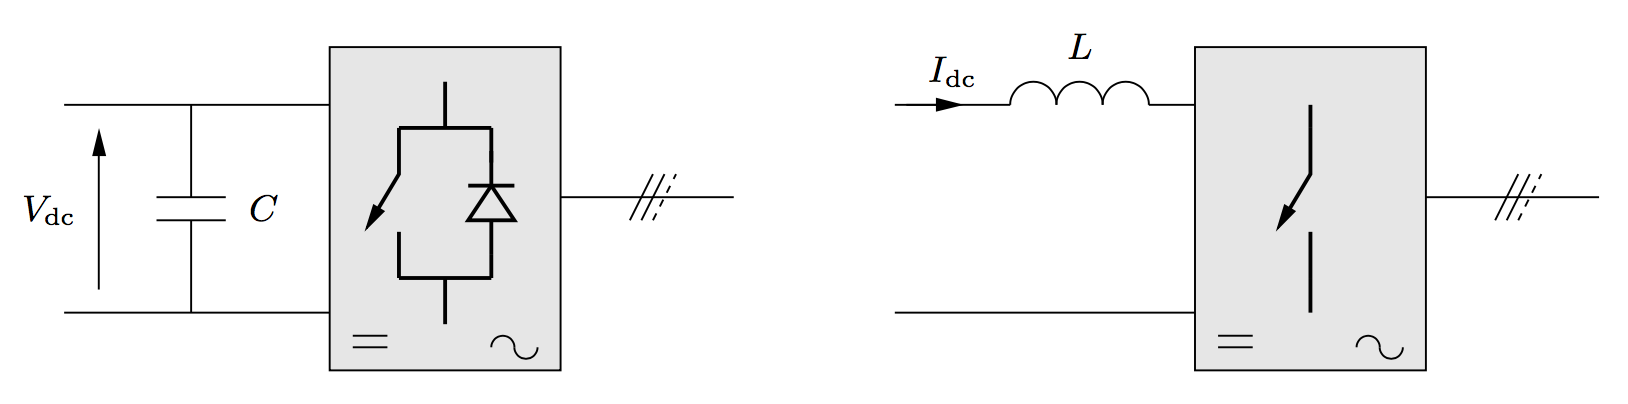
\includegraphics[scale=0.35]{ch4/1}
		\captionof{figure}{}
		\end{wrapfigure}
		It's the flow between two infinite parallel plates whiwh is driven by either a body force or a pression gradient. We will see that they can be linked together. We make the assumption that the flow is a \textbf{constant density flow} and \textbf{steady}. To analyse this, we need to choose a coordinates system. 

		\paragraph{Coordinates system}		
		We take $x_1$ in the direction of the driving force ($\rightarrow$) and $x_2$ normal to the plates, with the origin at the middel of the two plates. This is a planar flow, so
		\begin{equation}
			\Rightarrow  \frac{\D}{\D x_3}=0 \qquad and \qquad u_3 = 0 \mbox{ assumption}. 
		\end{equation}
		
		Because of the infinite plates, the origin can be everywhere on $x_1$ axis and the solution may not depend on it 
		\begin{equation}
			\frac{\D}{\D x_1} = 0 \qquad \mbox{(fully developed flow)}.
		\end{equation}
		This would not be the case if we had an entrance because the region near the entrance is not fully developed, we can see it as a transitory. Now let's make a momentum balance in a small region on $x_1$.
		
		\paragraph{$\mathbf{x_1}$ momentum balance}
			The time rate of change of the momentum inside a control volume + the net momentum flux going out is equal to 0 because there is no rate of change (steady) and the flow out is equal to the flow in (fully developed) 
			\begin{equation}
				0 = \mbox{sum of forces in } x_1.
			\end{equation}			 
		
		\paragraph{Mass balance} 
		It is the mass flow time rate of change + the mass out - mass in, the second and third term beeing null because velocity is constant
		\begin{equation}
			0 + \underbrace{\rho u_12x_2 |_{x_1+dx_1}- \rho u_12x_2 |_{x_1} }_{= 0} + \underbrace{\rho u_2 (x_1,x_2) -\rho u_2 (x_1,-x_2)}_{= 0} = 0.
		\end{equation}
		The third term teaches us that $2 \rho u_2(x_2)= 0 \Rightarrow u_2(x_2) = 0$. The other way to see that is to take the other form of the mass balance 
		\begin{equation}
			\cancel{\frac{\D\rho u_1}{\D x_1}}+\frac{\D\rho u_2}{\D x_2} = 0\qquad \Rightarrow \rho u_2 = cst = 0 \mbox{ (wall condition)}. 
		\end{equation}
		
		\begin{wrapfigure}[7]{l}{5.5cm}
		\vspace{-15mm}
		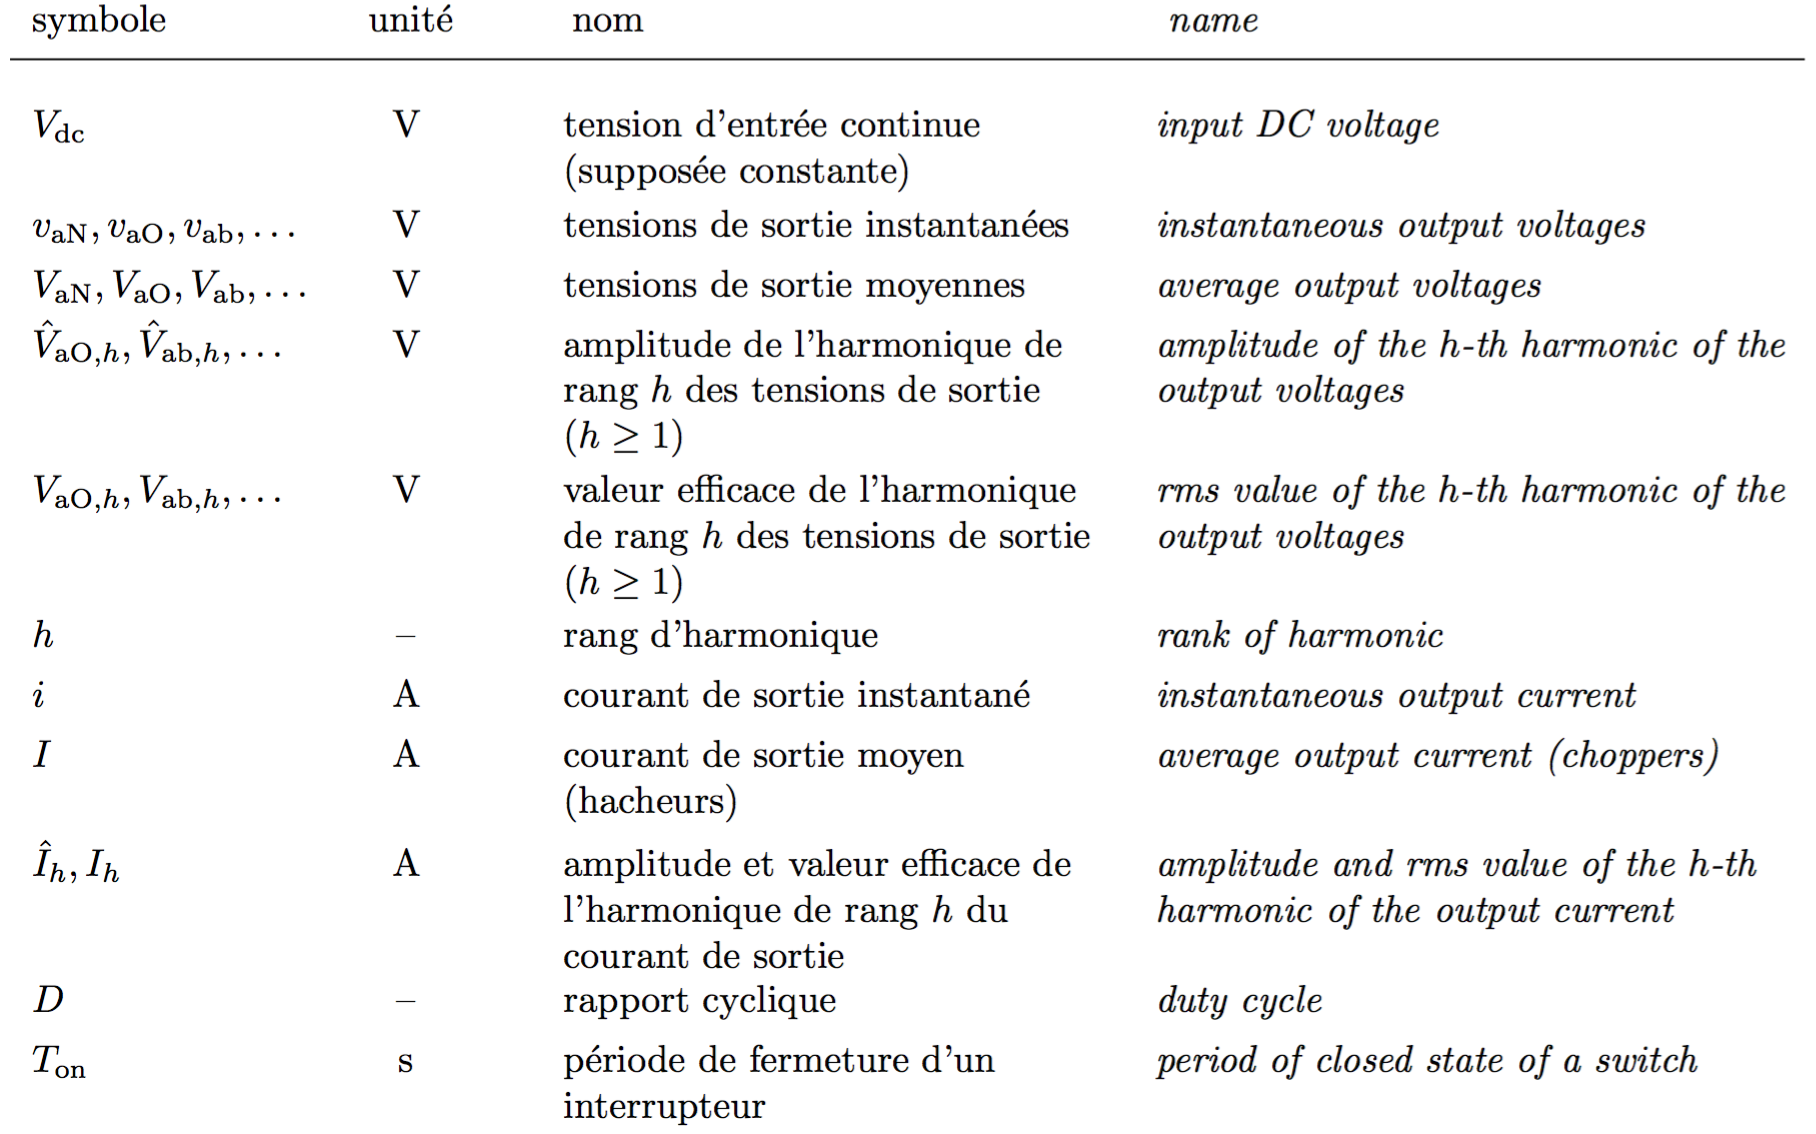
\includegraphics[scale=0.25]{ch4/2}
		\captionof{figure}{}
		\end{wrapfigure}
		\paragraph{Forces} There is the body force of acceleration $a \Rightarrow f_1 = am = a 2x_2 L \rho$, the pressure gradient $f_2 = (p_(0)-p(L))2x_2$ and the shear stress on the walls $f_3 = 2\tau L$, so
		\begin{equation}
		\begin{aligned}
			(p(0)-p(L))2x_2 +  a 2x_2 L \rho + 2\tau L = 0 \\
			\Rightarrow \tau = -x_2 \left( \rho a - \frac{p(L)-p(0)}{L}\right) = -x_2 f_1
		\end{aligned}
		\end{equation}
		\ \\
			
		\begin{wrapfigure}[7]{r}{5cm}
		\vspace{-15mm}
		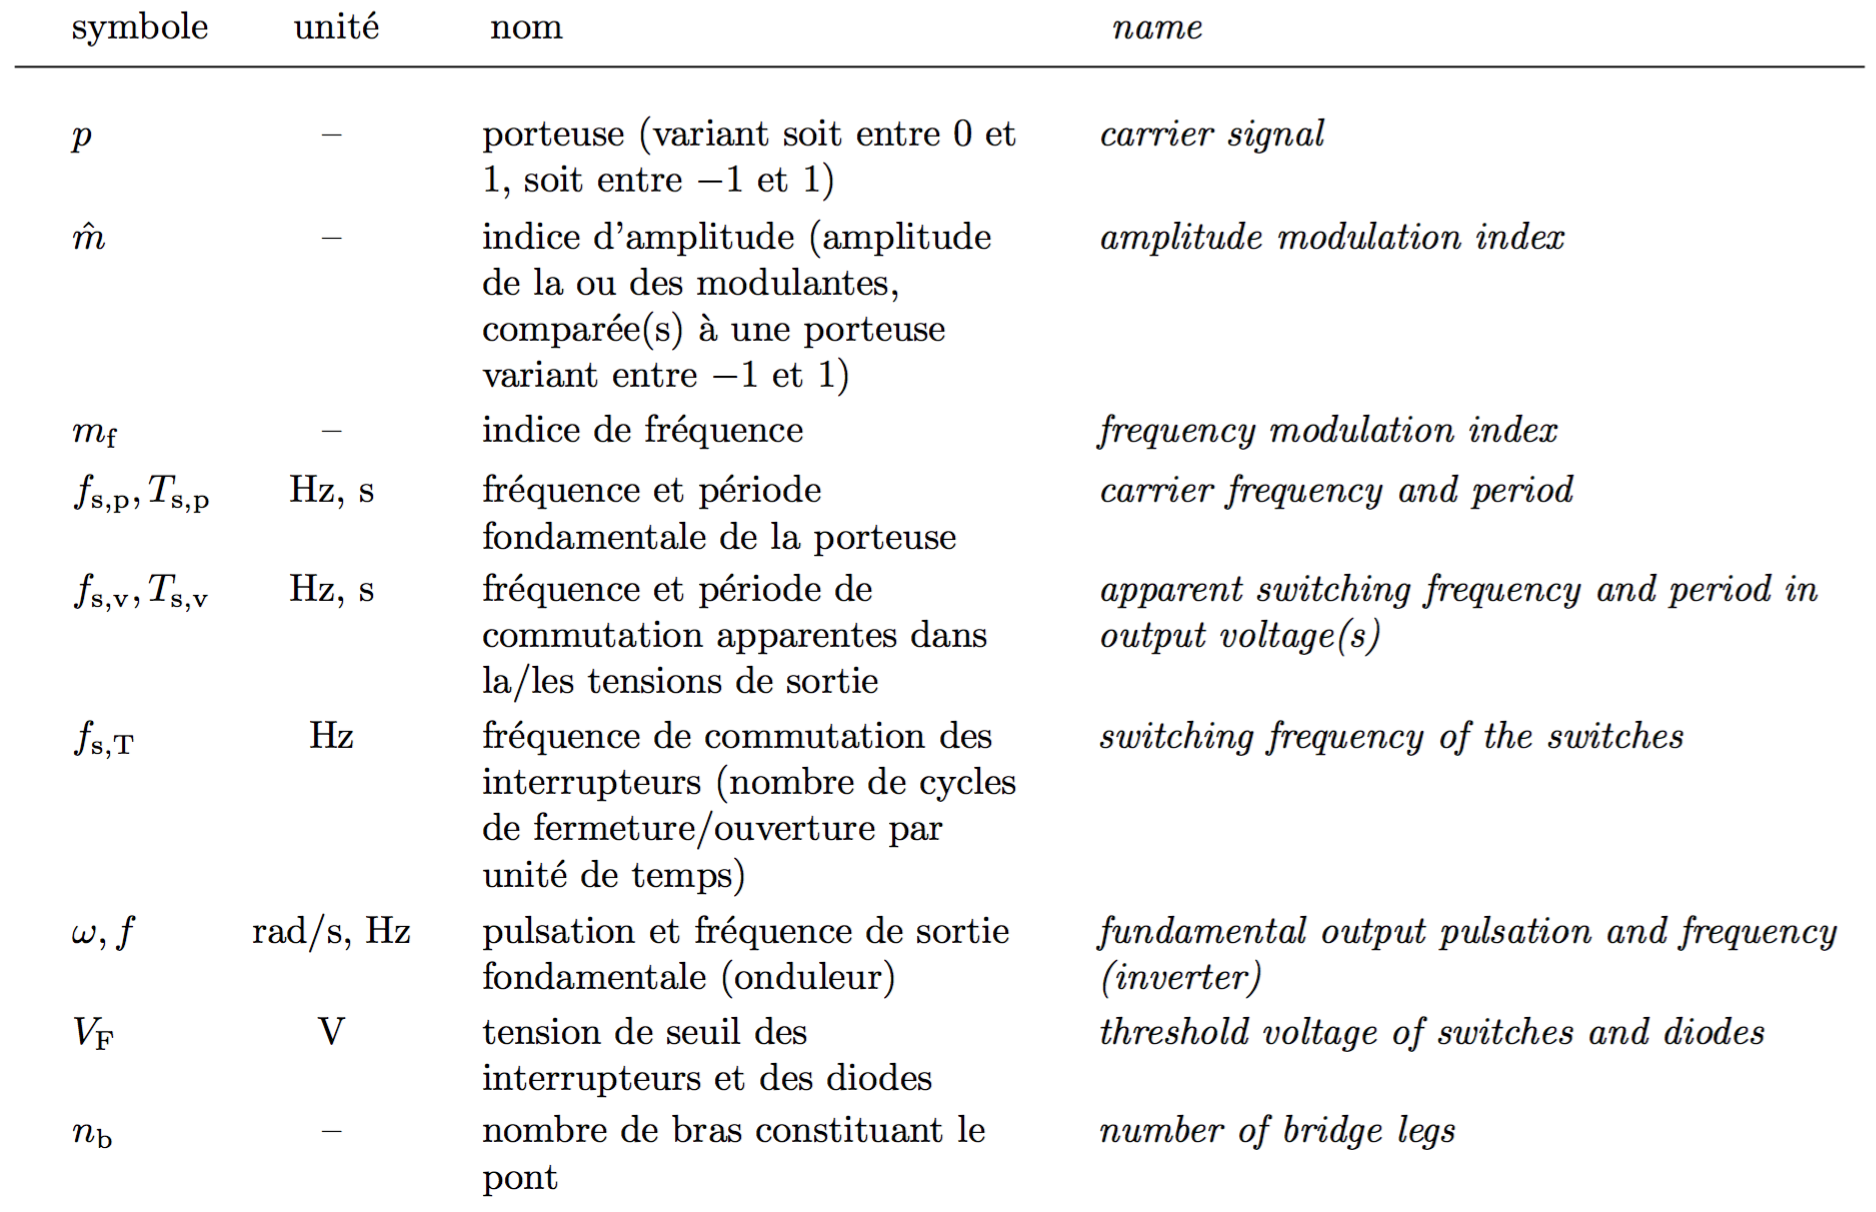
\includegraphics[scale=0.2]{ch4/3}
		\captionof{figure}{}
		\label{fig:4.3}
		\end{wrapfigure}
		where $f_1 = \rho a - \frac{dp}{dx} = -\frac{d\hat{p}}{dx}$ is the driving force (force per unit volume) and $\hat{p} = p - \rho a$ the driving pressure, we see that even the pressure gradient appears in his expression. The evolution of the linear $\tau$ is represented on \autoref{fig:4.3}, shear stress representing the effect of the upper part on the lower part, it seems legit to have $-\tau$ for the upper wall meaning that the wall slows down the fluid (below the fluid drag the wall). The velocity profile can be found as 
		\begin{equation}
			\tau = -x_2 f_1 = \mu \left( \frac{\D u_1}{\D x_2}+ \cancel{\frac{\D u_2}{\D x_1}}\right) \qquad \Rightarrow \mu \frac{\D u_1}{\D x_2} = -x_2 f_1 \Leftrightarrow u_1 = \frac{f_1}{2\mu} (-x_2^2+cst).
		\end{equation}
		
		\begin{wrapfigure}[7]{r}{3.6cm}
		\vspace{-5mm}
		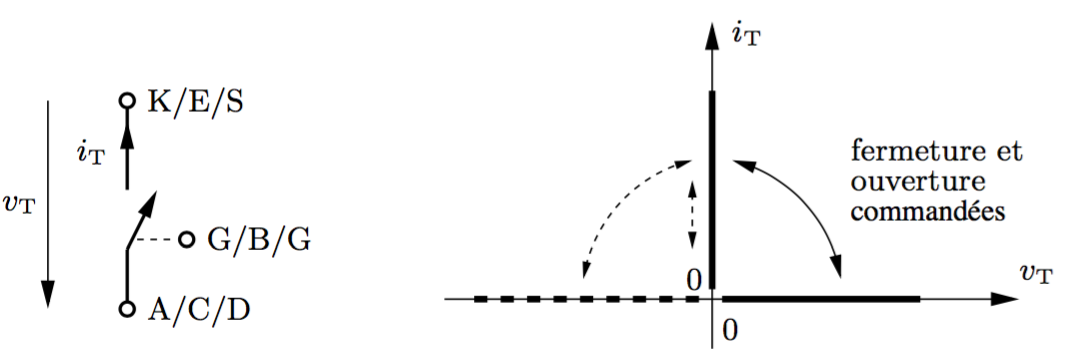
\includegraphics[scale=0.2]{ch4/4}
		\captionof{figure}{}
		\label{fig:4.4}
		\end{wrapfigure}
		The non slip boundary condition at the wall gives $u_1(\pm \frac{h}{2}) \Rightarrow c =\left( \frac{h}{2}\right)^2$. The velocity profile is 
		\begin{equation}
			u_1 = \frac{f_1}{2\mu} \left(\left(\frac{h}{2}\right)^2-x_2^2\right)
			\label{eq:4.8}
		\end{equation}
		which is parabolic as shown on \autoref{fig:4.4} with a maximum on $x_1$ axis of value $u_1 = \frac{f_1h^2}{8\mu}$. It is also interesting to compute the volume flow per unit span $[m^2/s]$ ($x_3$) 
		\begin{equation}
			\dot{V} = \int _{-h/2}^{h/2} u_1 \, dx_2 = \frac{2}{3} h \frac{f_1h^2}{8\mu} = \frac{f_1h^3}{12\mu} 
		\end{equation}
		where the integral has been computed using the definition of the era of the parabole $2/3 \times h \times u_c$. 
		
		\paragraph{Dimensional analysis}
		Imagine that we would have liked to determine the velocity profile by dimensional analysis. The veloity dependance is 
		\begin{equation}
			u_1 = f(x_2, f_1, h, \mu ,\rho )
		\end{equation}
		giving us 6 variables and 3 physical dimensions and so 3 dimensionless groups.   To make the velocity dimensionless, we computed the velocity at the center, let's use it. The dimensionless velocity will be function of 2 dimensionless groups 
		\begin{equation}
			\frac{u_1}{\frac{f_1h^2}{8\mu}} = \varphi \left( \frac{2x_2}{h}, Re = \frac{u_c h}{\nu} = \frac{\rho f_1 h^3}{8 \mu ^2} \right).			
		\end{equation}		 
		Now if we rewrite \eqref{eq:4.8} as 
		\begin{equation}
			u_1 = \frac{f_1h^2}{8\mu}\left( 1 - \left( \frac{2x_2}{h}\right) ^2\right).
		\end{equation}
		
	 	\begin{wrapfigure}[10]{l}{3.6cm}
		\vspace{-5mm}
		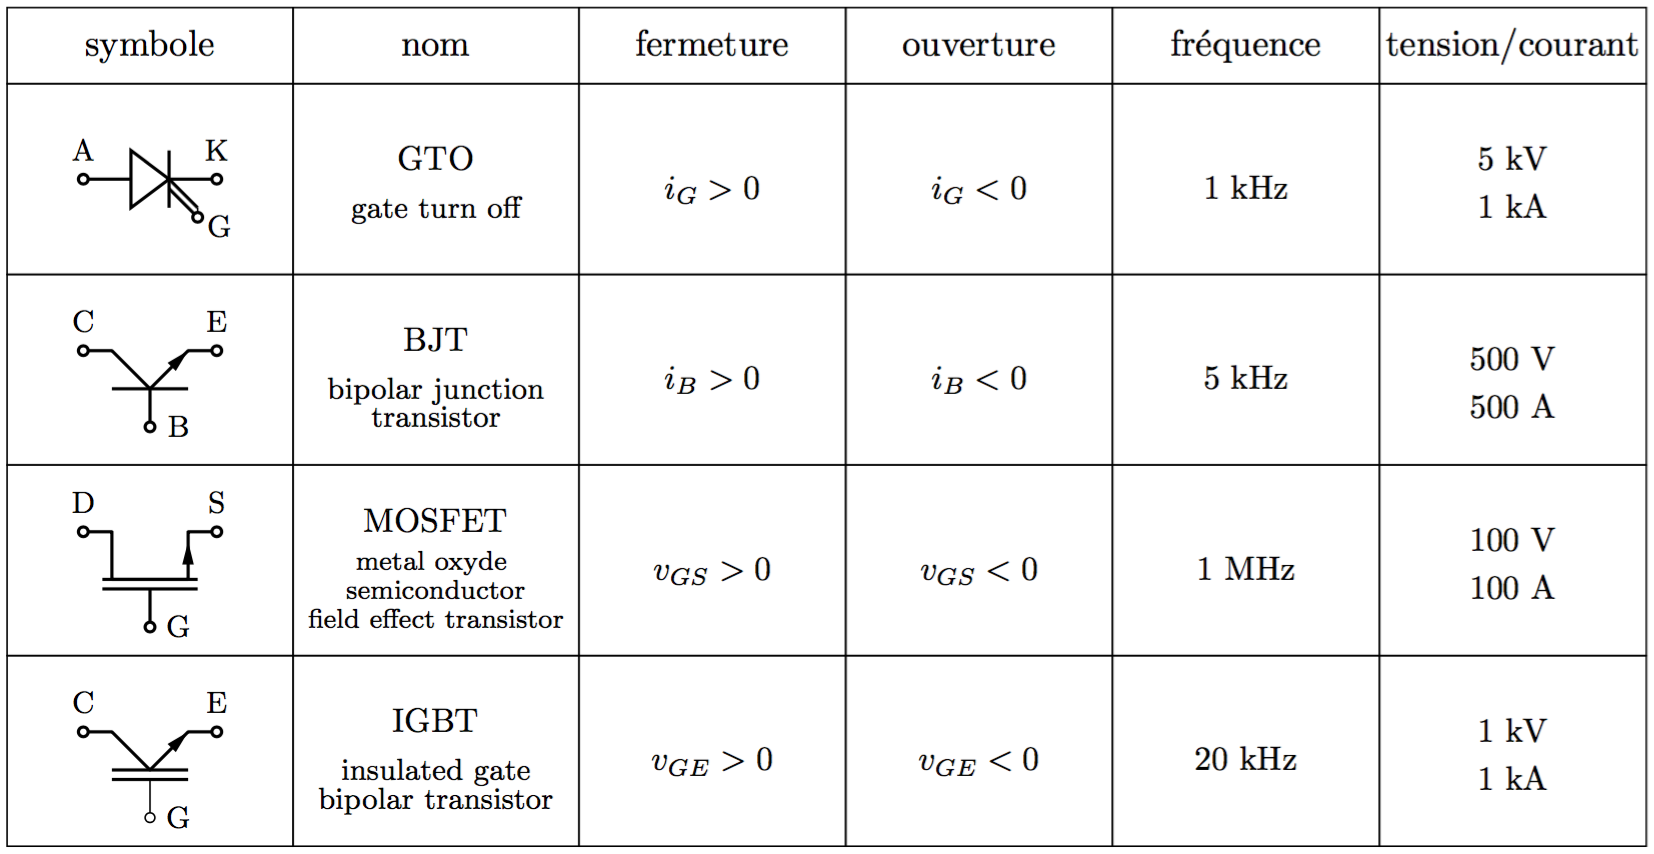
\includegraphics[scale=0.2]{ch4/5}
		\captionof{figure}{}
		\end{wrapfigure}
		When we compare the 2 equations, we see that $\varphi = f(x_2/h)$. That means that when we solve the equation there is no dependance on the Re number. So the dimensional analysis doesn't give the full information, we have to solve. Re number is the ratio between viscous forces and conventional inertial forces. Because of fully developed criteria there is no conventional inertial forces, it is normal so that the flow does not depend on the Re number. This parabolic profile is respected for low velocities but disturb when velocity increases. We made the assumption that the flow is steady, but for a certain velocity the flow is no longer steady, it becomes chaotic (turbulences). 
		

\section{Macroscopique des cription of turbulent flows - Reynolds decomposition}
	The interest of this approach is in the mean flow, in average quantities. The idea is to repeat the experiment several times and make a statistical average in order to decompose all variables into an average and a fluctuation. This is called the Reynolds decomposition
	\begin{equation}
	\begin{array}{c}
		\forall \ quantity \ q : \langle q(x_1,x_2,x_3,t)\rangle =  \frac{1}{N} \sum _{k=1}^N q_k(x_1,x_2,x_3,t)\\ \\
		and \\ \\
		q_k(x_1,x_2,x_3,t) = \underbrace{\langle q_k(\cdots )\rangle}_{average} + \underbrace{q_k(\cdots )}_{fluctuation}
	\end{array}
	\end{equation}
	where $k$ is the experiment index. We are going to derive equations for the average properties for statistically steady flows (such that $\frac{\D \langle q\rangle}{\D t} = 0$). We can consider the time average with a certain period $T$
	\begin{equation}
		\bar{q}_T (x_1,x_2,x_3,t) = \frac{1}{T} \int _{t-T/2}^{t+T/2} q(x_1,x_2,x_3,t) \, dt
	\end{equation}
	which "smooth" the signal by keeping only large time scale fluctuations. For statistically steady flows, the \textbf{ergodicity hypothesis} is valid 
	\begin{equation}
		\lim _{T\rightarrow \infty} \bar{q}_T =  \langle q \rangle .
	\end{equation}
	For statistically unsteady flows, it is valid only if $T$ is much larger than the turbulent fluctuations time scale and much smaller than the average motion time scale. 
	
	\subsubsection{Properties of the averaging operator}

\begin{itemize}
\item[•] \textbf{Linearity :}
\begin{equation}
\langle a q_1 + bq_2\rangle = a \langle q_1\rangle + b  \langle q_2 \rangle 
\end{equation}

\item[•]
\begin{equation}
\langle \langle q\rangle \rangle = \langle q \rangle 
\end{equation}

\item[•]
\begin{equation}
\langle q'\rangle  = 0 \qquad as \qquad \langle q \rangle = \langle \langle q\rangle  + q'\rangle = \langle \langle q \rangle \rangle + \langle q'\rangle  =  \langle q\rangle  + \langle q'\rangle  \Rightarrow \langle q'\rangle  = 0
\end{equation}

\item[•]
\begin{equation}
\langle\langle q_1\rangle q_2\rangle = \langle q_1 \rangle \langle q_2\rangle
\end{equation}

\item[•] \textbf{Commutativity with differential operators}
\begin{equation}
	\left\langle \frac{\D q}{\D x_1} \right\rangle = \frac{\D \langle q \rangle}{\D x_1} \qquad \left\langle \frac{\D q}{\D t} \right\rangle = \frac{\D \langle q \rangle}{\D t}
\end{equation}
\end{itemize}

\subsubsection{Average continuity equation}
	Let's remind that we are considering \textbf{constant density} flow. In this case the governing equation for mass is
	\begin{equation}
		\cancel{\dot{\rho}} + \rho \nabla \vec{u} = 0 \qquad \Rightarrow \nabla \vec{u} = 0 = \frac{\D u_i}{\D x_i}
	\end{equation}
	Let's average this out 
	\begin{equation}
		\left\langle \frac{\D u_i}{\D x_i}  \right\rangle = \left\langle \frac{\D u_1}{\D x_1} + \frac{\D u_2}{\D x_2} + \frac{\D u_3}{\D x_3} \right\rangle = 		\left\langle \frac{\D u_1}{\D x_1}  \right\rangle  + \left\langle \frac{\D u_2}{\D x_2}  \right\rangle  + 	\left\langle \frac{\D u_3}{\D x_3}  \right\rangle  = 0
	\end{equation}
	and using the commutativity with differantial operators, we have the 
	\begin{center}
	\theor{\textbf{Average of the continuity equation}
	\begin{equation}
		\frac{\D \langle u_i \rangle}{\D x_i} = 0
	\end{equation}
	}
	\end{center}
	This is exactly what we need because we have only average velocity field. 
	
	\subsubsection{Average momentum equation}
		The conservation form of the equation without considering body force is
		\begin{equation}
			 \frac{\D \rho u_i}{\D t} + \frac{\D \rho u_i u_j}{\D x_j} = \rho \left[ \frac{\D u_i}{\D t} + \frac{\D u_iu_j}{\D x_j} \right] = - \frac{\D p}{\D x_i} + \frac{\D \tau _{ji}}{\D x_j}.
		\end{equation}
		
		Let's average this out 
		\begin{equation}
			\rho \left[ \frac{\D \langle u_i\rangle}{\D t} + \frac{\D \langle u_iu_j\rangle}{\D x_j} \right] = - \frac{\D \langle p\rangle}{\D x_i} + \frac{\D \langle \tau _{ji}\rangle}{\D x_j} \qquad with \qquad 
			\begin{aligned}
				\tau _{ji} &= \mu \left( \frac{\D u_i}{\D x_j} + \frac{\D u_j}{\D x_j}\right) \\
			\langle \tau _{ji} \rangle &= \mu \left( \frac{\D \langle u_i \rangle}{\D x_j} + \frac{\D \langle u_j \rangle}{\D x_j}\right)	
			\end{aligned}
			\label{eq:4.25}
		\end{equation}
		This was easy game, let's now concentrate on $\langle u_i u_j \rangle$ by considering the Reynolds decomposition
		\begin{equation}
		\begin{aligned}
			\langle u_i u_j\rangle &= \left\langle (\langle u_i \rangle + u_i') (\langle u_j \rangle + u_j' )  \right\rangle \\
 &= \langle  \langle u_i \rangle \langle u_j \rangle + \langle u_i \rangle u'_j + u_i' \langle u_j \rangle + u_i' u_j'\rangle\\ 
&= \langle u_i\rangle \langle u_j \rangle + \underbrace{\langle \langle u_i \rangle u'_j \rangle}_{=0} +\underbrace{\langle  u_i' \langle u_j \rangle \rangle }_{=0} + \underbrace{\langle u_i' u_j'\rangle}_{\neq 0} \\
		\end{aligned}
		\end{equation}
		The last term is clearly $\neq 0$ as if $i=j$ we have the average of a square wich is never 0 when $u\neq 0$. If now we replace this in \eqref{eq:4.25}, we have
		\begin{equation}
			\rho \left[ \frac{\D \langle u_i\rangle}{\D t} + \frac{\D \langle u_i\rangle \langle u_j\rangle}{\D x_j} + \frac{\D \langle u_i' u_j' \rangle}{\D x_j} \right] = - \frac{\D \langle p\rangle}{\D x_i} + \frac{\D \langle \tau _{ji}\rangle}{\D x_j}
		\end{equation}
		and we see that in fact we still have fluctuations in the average momentum equation. But we see that we have essentially the same equation as for laminar, normal viscous flows and an extra term. Remind that we interpretated $\rho \langle u_i \rangle \langle u_j \rangle$ as beeing the \textbf{average momentum flux tensor} and $\frac{\D \langle \tau _{ji} \rangle}{\D x_j}$ was the \textbf{molecular agitation momentum fluxes}. So the fluctuations results in an additional momentum flux tensor called the \textbf{turbulent fluctuation momentum fluxes}. If we bring this term to the right side, we have the
		
		\begin{center}
		\theor{
		\textbf{Average momentum equation}
		\begin{equation}
					\rho \left[ \frac{\D \langle u_i\rangle}{\D t} + \frac{\D \langle u_i\rangle \langle u_j\rangle}{\D x_j} \right] = - \frac{\D \langle p\rangle}{\D x_i} + \frac{\D}{\D x_j}\left( \langle \tau _{ji}\rangle - \rho \langle u_i' u_j' \rangle\right)
		\label{eq:4.28}
		\end{equation}
		}
		\end{center}
		where we can see the term as additional stresses called the \textbf{Reynolds stresses} $T_{ij}^R$.
		
		\subsubsection{Channel flow}
			Let's come back to the channel flow which is statistically steady and fully developed. So, reminding that $u_2 = 0$ the $i=1$ momentum equation reduces to
			\begin{equation}
				\frac{\D \langle u_1 \rangle ^2}{\D x_1} = 0 = \underbrace{-\frac{\D \langle p \rangle}{\D x_1}}_{f_1} + \frac{\D}{\D x_2}\underbrace{\left( \langle \tau _{21}\rangle - \rho \langle \tau ^R_{21} \rangle\right)}_{\tau _{21}^{tot}} \qquad \Rightarrow \tau _{21}^{tot} = -f_1 x_2
			\end{equation}			 
			which is exactly the same expression as we obtained before at the difference that now we have to consider in addition the new stresses. 
			
	
\section{Average velocity profiles in turbulent wall-bounded shear flows}
	We've seen that for the channel flow in laminar flow we obtained a parabolic velocity profile. It is also the case for a flow in a pipe for laminar flow. Many measure instruments do the averaging process by themself. In the turbulent case, the profiles are much more flatter/uniform even in the channel flow. This can be explained by turbulence. Indeed, the agitations play the role of an agitator, they exchange the momentum neighboring there they do mixing/homogenise so the velocity is more uniform. The consequence is that velocity has to fall down more rapidly close to the wall where the only shear is the molecular shear (no fluctuation), leading to increased friction. Another observation is that contrary to the case of laminar flows, the parabole is no longer independant to the Re number. We will try to express the velocity profile in turbulent flow and for this we will consider a channel flow 
	
	\subsection{Channel flow}
		Let's start with the average momentum equation \eqref{eq:4.28} that simplifies knowing that the flow is statistically steady and fully developed, we have
		\begin{equation}
			0 = -\frac{\D \langle p \rangle}{\D x_1} + \frac{\D}{\D x_2} \left( \langle \tau _{21}\rangle - \rho \langle u_1' u_2' \rangle\right)\qquad \Rightarrow \tau _{21}^{tot} = -f_1 x_2
		\end{equation}
		leading to the linear relation we found next time for $\tau _{21}^{tot}$. 
		
		\begin{center}
		\begin{minipage}{0.49\textwidth}
		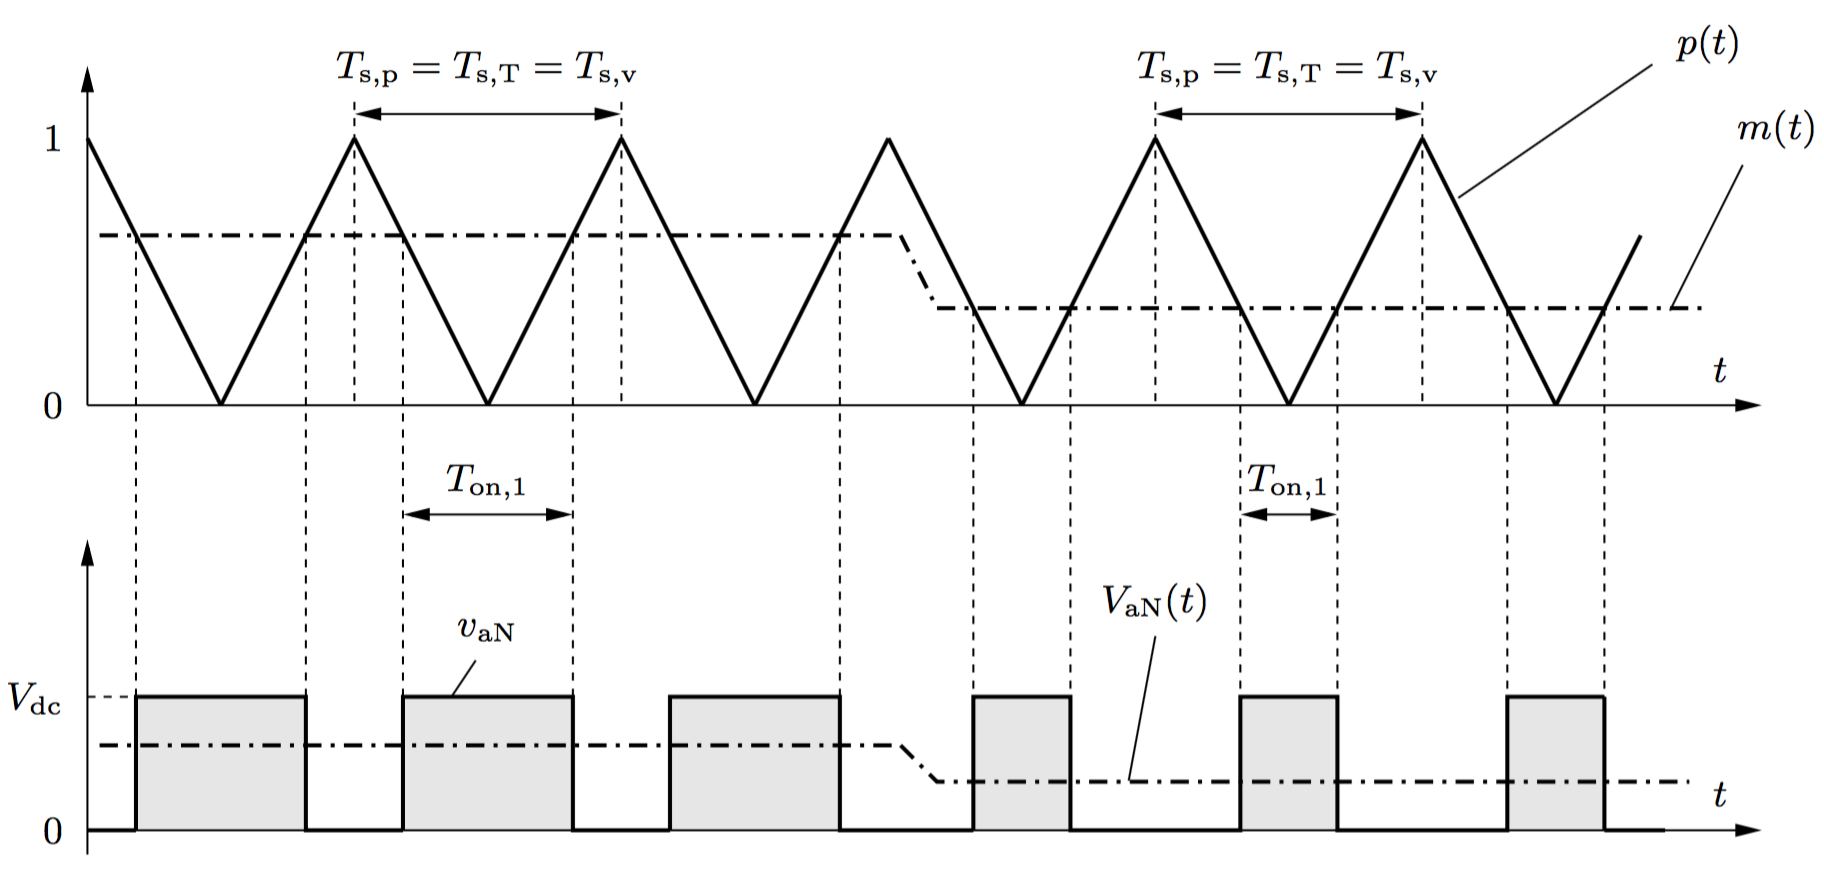
\includegraphics[scale=0.25]{ch4/6}
		\captionof{figure}{}
		\label{fig:4.6}
		\end{minipage}
		\begin{minipage}{0.49\textwidth}
		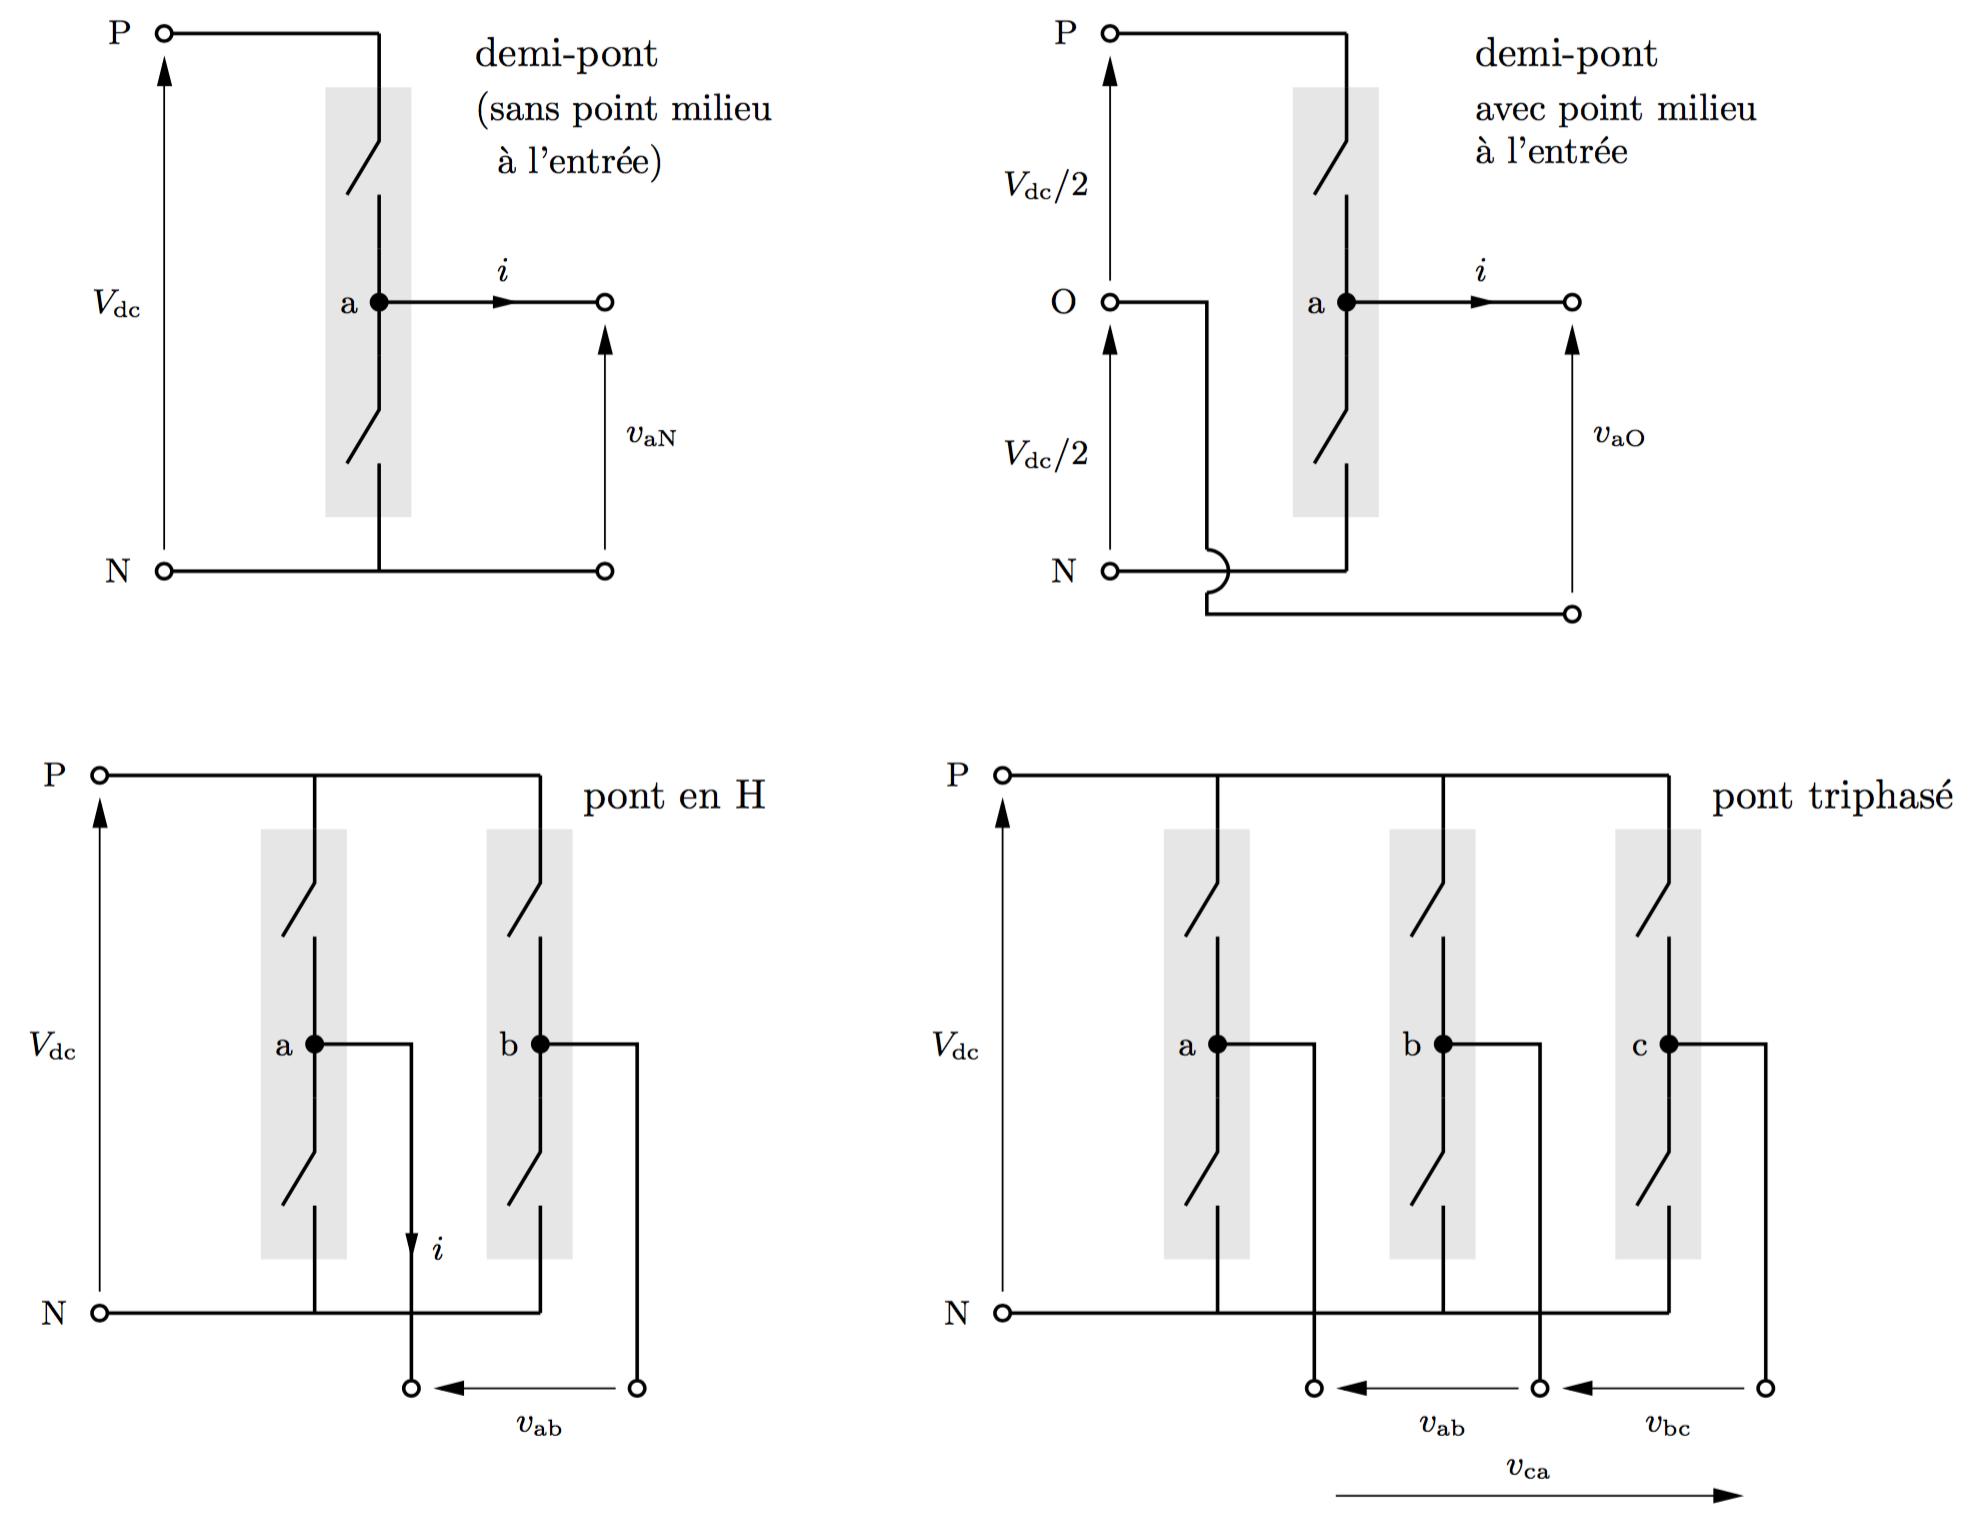
\includegraphics[scale=0.41]{ch4/7}
		\captionof{figure}{}
		\label{fig:4.7}
		\end{minipage}
		\end{center}
		
		The channel can be decomposed in several zones, namely the central zone where the total stress is nearly only the Reynold stress, there is hardly no conrtibution of the viscous stress. Then there is a region close to the wall where this last becomes dominant. The reason why the velocity profile is dependent of the Re number is that these two stresses doesn't vary in the same way with Re. \autoref{fig:4.6} represents the Re stress, the totally linear one beeing the total stress, so the viscous stress is null in the center whereas it increases near the wall (where Re stress decreases). We decompose the channel in an \textbf{outer zone }where $\tau _{21}^{tot} \approx \tau _{21} ^R = -\rho \langle u_1'u_2' \rangle$ and an \textbf{inner zone} where both stresses are significant. \autoref{fig:4.7} consists in a zoom on the left inner zone. \\
		
		We will now use dimensional analysis to find the velocity profile in the two regions. Let say that the average velocity at a point on the channel is a function of 
		\begin{equation}
			\langle u \rangle = f\left(y, \sqrt{\frac{\tau _{wall}}{\rho}} = u_{\tau}, \nu , u_c , h\right)
		\end{equation}
		Depending on the region, this function will change 
		\begin{equation}
			inner :  \langle u \rangle = f\left(y, \sqrt{\frac{\tau _{wall}}{\rho}} = u_{\tau}, \nu, \cancel{u_c}, \cancel{h}\right) \qquad outer : \langle u \rangle = f\left(y, \sqrt{\frac{\tau _{wall}}{\rho}} = u_{\tau}, \cancel{\nu}, u_c , h\right)
		\end{equation}
		where $u_\tau$ is the friction velocity. 

	\subsection{Inner zone (smooth wall)}
		If we look at our reduced function, this involves 4 quantities and 2 physical dimensions, leading to two dimensionless groups 
		\begin{equation}
			u^+ \equiv \frac{\langle u \rangle}{u_\tau} = f\left(Re = \frac{y u_\tau }{\nu}\equiv y^+\right)
		\end{equation}		 
		where $u^+$ and $y^+$ are the wall units, notation in litterature for these dimensionless groups. The inner zone can be decomposed into three sublayer as indicated on \autoref{fig:4.7} :\\
		\begin{itemize}
			\item[•] \textbf{the viscous sublayer (1) :} very close to the wall, where $\langle \tau _{21} ^V \rangle \gg \langle \tau _{21} ^R \rangle $
			\item[•] \textbf{the buffer layer (2) :} the transition layer where $\langle \tau _{21} ^V \rangle \approx \langle \tau _{21} ^R \rangle $ 
			\item[•] \textbf{the overlap layer (3) :} where $\langle \tau _{21} ^V \rangle \ll \langle \tau _{21} ^R \rangle $
		\end{itemize}
		
		\subsubsection{Viscous sublayer (1)}
			This layer is so small and close to the wall that 	
			\begin{equation}
			\begin{array}{cccc}
				&\tau _{21} ^{tot}(y)= \mu \frac{\D \langle u \rangle }{\D y} \approx \tau _{wall}  &\Leftrightarrow  &\frac{\mu}{\rho}\frac{\D \langle u \rangle }{\D y} = \frac{\tau _{wall}}{\rho} = u_\tau ^2\\
				\Leftrightarrow &\nu \langle u \rangle = u^2_{\tau} y &\Leftrightarrow  &\frac{\langle u \rangle }{u_\tau} = \frac{u_\tau y}{\nu}
			\end{array}
			\end{equation}
			This means that here we have the final result 
			\begin{equation}
				u^+ = y^+
			\end{equation}
			
		\subsubsection{Overlap layer (3)}
			There viscosity does not play a role. In other words, we expect that 
			\begin{equation}
				\frac{\D \langle u \rangle}{\D y} = f'\left(y, u_\tau , \cancel{\nu}\right) \qquad \Rightarrow \frac{y}{u_\tau}\frac{\D \langle u \rangle}{\D y} \approx cst = \frac{1}{\kappa}.
			\end{equation}
			So if we make appear the wall notations, we have
			\begin{equation}
				\frac{u_\tau^2}{\nu}\frac{\D u^+ }{\D y^+} = \frac{1}{\kappa}  \frac{u_\tau}{y} \qquad\Rightarrow \frac{\D  u^+}{\D y^+} = \frac{1}{\kappa}\frac{\nu}{yu_\tau} = \frac{1}{\kappa y^+} \qquad \Rightarrow u^+ = \frac{1}{\kappa}\ln y^+ + B.
				\label{eq:4.37}
			\end{equation}
						
		\begin{wrapfigure}[8]{l}{5cm}
		\vspace{-5mm}
		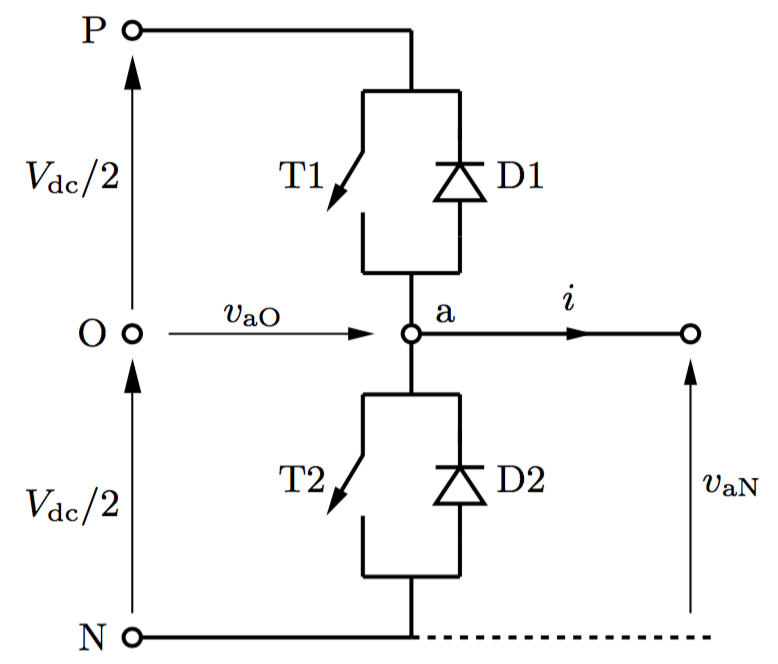
\includegraphics[scale=0.2]{ch4/8}
		\captionof{figure}{}
		\label{fig:4.8}
		\end{wrapfigure}
		This is theory, let's check what theory says about. When we look at the diagram, our theory matches roughly with the linear (in $\log$) for $50\leq y^+ \leq 500$. For the viscous sublayer represented by the exponential, the curves matches till $y^+ \approx 5$ wall units. That's very small (1/10 - 1/100 of the overloop). There is a smooth transition between the two curves. 
		
	\	\\ \subsubsection{Buffer layer (2)}
			The idea is to rewrite the expression of the two zones but with $y^+ = f(u^+)$ 
			\begin{equation}
			\begin{aligned}
				&viscous \ layer : y^+ = u^+\\
				&overloop \ layer : y^+ =  \exp (\kappa(u^+ - B))= \exp (\kappa u^+)\exp (-\kappa B)
			\end{aligned}
			\end{equation}
			We can have a good transition between the two by 
			\begin{equation}
				y^+ = u^+ + \exp (-\kappa B)\left[ \exp(\kappa u^+) - \underbrace{\left( 1 + \kappa u^+ +  \frac{(\kappa u^+)^2}{2}  +  \frac{(\kappa u^+)^3}{6}\right)}_{taylor \ serie \ expansion \ of\ \exp(\kappa u^+)}\right]
			\end{equation}
			Indeed when $\kappa u^+$ is small, the second part will be negligible regarding $u^+$ and for high, we found the overlap layer. To have the smooth transition, only two terms are enough but taking more leads to a best fitting with the practice. 
			
	
	\subsection{Inner zone (rough wall)}
		The wall are never exactly smooth in rality. We already discussed that to have exact similarity between the model and the prototype we must have the same relative rougness ($\lambda /L$). Let's see the effect on velocity profile. In practice it is impossible to do an exhaustive study because of the number of parameters. There is also various forms of roughness: \\
		
		\begin{itemize}
			\item[•] \textbf{uniform sand roughness:} when you blew sand particles on a paper for example 
			\item[•] \textbf{non uniform sand roughness:} when particles have different scale and form
			\item[•] \textbf{periodic roughness:} this can be obtained for example if we put wires or square ribs at regular interval. \\
		\end{itemize}
		
		We will consider the first one. In the overlap layer, we expect that \eqref{eq:4.37} remains correct but B will be function of $k^+$ which is $k$, the hight of the grains, in wall units (divided by the inner zone length scale)
		\begin{equation}
			u^+ = \frac{1}{\kappa}\ln y^+ + B_1(k^+) \qquad with \qquad k^+ =k \frac{u_\tau}{\nu}
		\end{equation}
		We expect that roughness will slow down the fluid meaning that $B_1(k^+) < B$. We can rewrite our equation as 
		\begin{equation}
			u^+ = \frac{1}{\kappa}\ln y^+ + B - \Delta u^+ (k^+) \qquad where \qquad \Delta u^+ (k^+) = B - B_1(k^+)
		\end{equation}
		where $\Delta u^+$ is the velocity deficit, expected to be $>0$.\\
		
		\begin{wrapfigure}[8]{l}{6.5cm}
		\vspace{-5mm}
		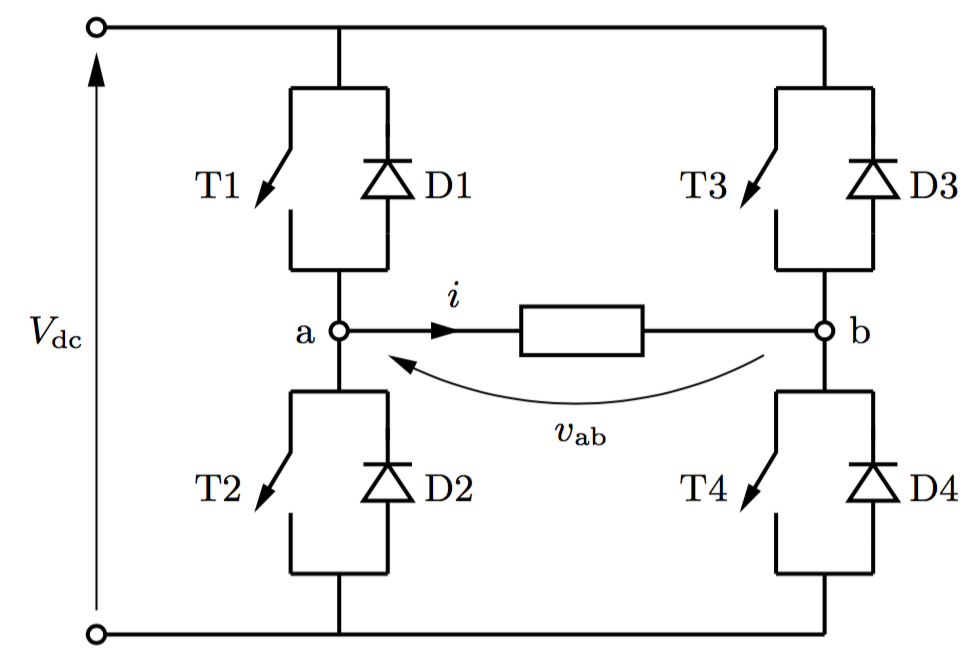
\includegraphics[scale=0.27]{ch4/9}
		\captionof{figure}{}
		\label{fig:4.9}
		\end{wrapfigure} 
		In experiments we see indeed that $\Delta u^+$ is a function of $k^+$ and depends on the type of roughness. In which we concerns, we have to look to the triangles. The first observation is that $\Delta u^+ = 0$ for $k^+ \leq 5$, so if the roughness is such that the hight doesn't exceed 5 in wall units, the fluid behaves exactly as the wall was smooth : \textbf{hydraulically smooth regime}. Let's remind that 5 is the upper limit of the viscous sublayer. The conclusion is that, as long as the grains remains barried within the viscous sublayer, roughness does not influence the average velocity profile. For non uniform roughness, there are bigger grains that goes throw this limit. 
		The second observation is that for higher $k^+$ ($\geq 80$) on the logarithmic axis $\Delta u^+$ respect a line of constant slope 
		\begin{equation}
			\Delta u^+ =  \frac{1}{\kappa} \ln k^+ + B_3 \qquad k^+ \geq 80 
		\end{equation}
		This means that the velocity profile in this zone is 
		\begin{equation}
			u^+   = \frac{1}{\kappa} \ln y^+ + B - \left(  \frac{1}{\kappa} \ln k^+ + B_3 \right) 
 		= \frac{1}{\kappa} \ln \frac{y^+}{k^+} + B - B_3  = \frac{1}{\kappa} \ln \frac{y}{k} + B - B_3 
		\end{equation}
		We see that the appropriate length scale changes from $\nu / u_\tau$ to beeing $k$ itself and this is called the \textbf{fully rough regime} where we can make another manipulation for $u^+$ 
		\begin{equation}
		\begin{array}{c}
			u^+ = \frac{1}{\kappa}\ln y^+ + B - \Delta u^+ (k^+)  = \frac{1}{\kappa}\ln \frac{y^+}{k^+} + \underbrace{B + \frac{1}{\kappa} \ln k^+ - \Delta u^+ (k^+)}_{B_2(k^+)} \\
			where \\\\
			k^+ \leq 5 \quad B_2(k^+) \approx B+\frac{1}{\kappa}\ln k^+ \qquad k \geq 80 \quad B_2(k^+) \approx B-B_3
		\end{array}
		\end{equation}
		
		\begin{wrapfigure}[10]{l}{5.8cm}
		\vspace{-2mm}
		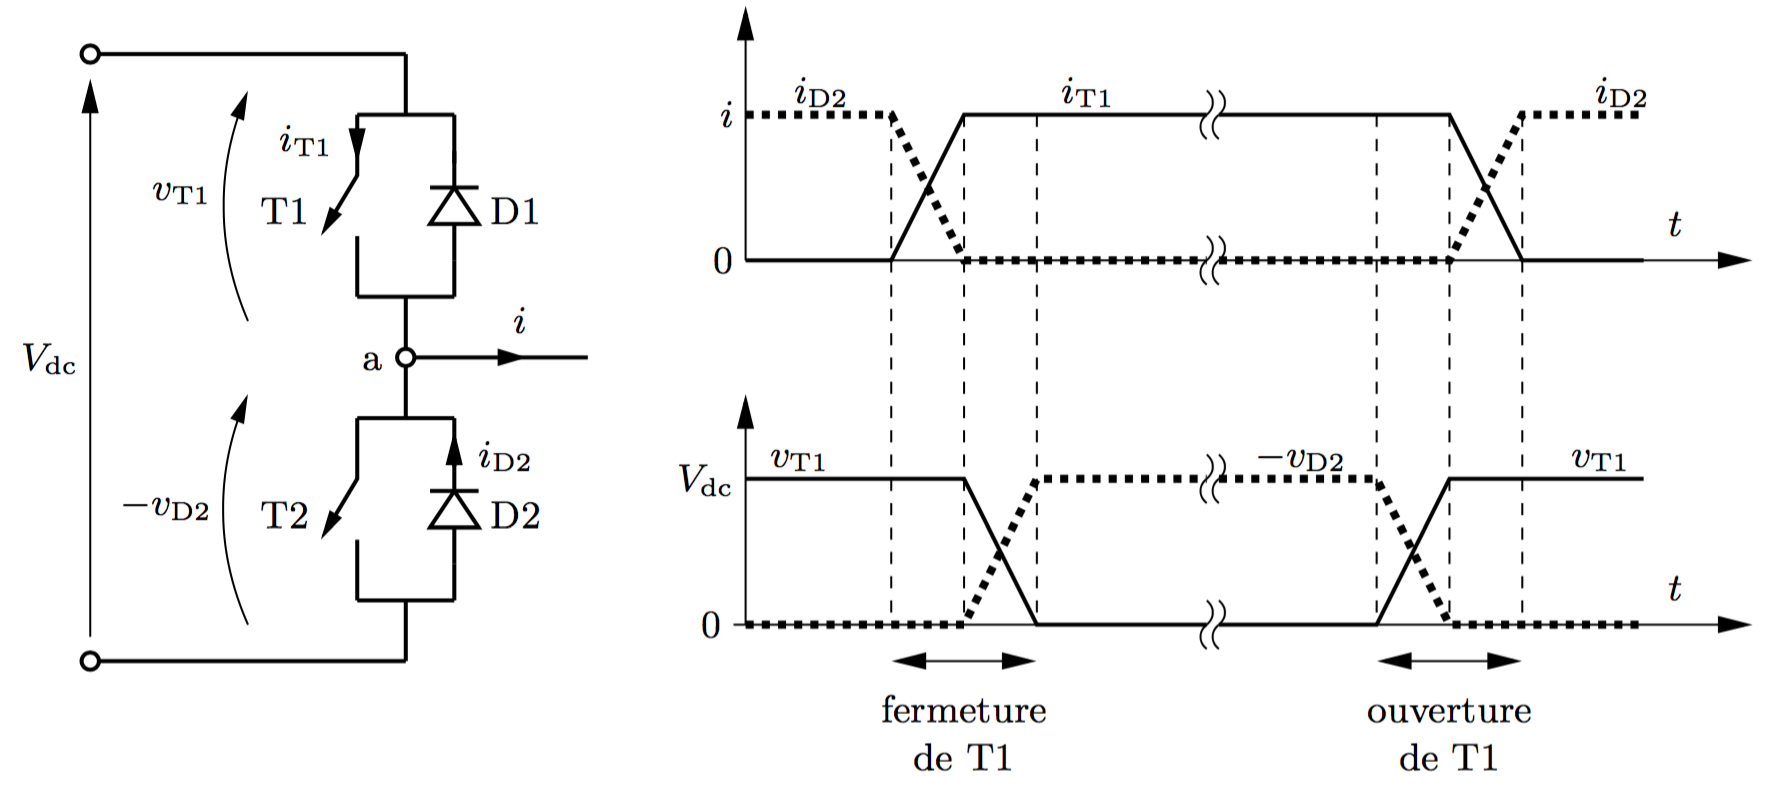
\includegraphics[scale=0.35]{ch4/10}
		\captionof{figure}{}
		\end{wrapfigure} 
		This is shown on this diagram where we have a linear curve for $k\leq 5$ giving $B = 5.5$ (y axis) and then the constant area ($k\leq 80$). Notice that we have an overshoot in the transitional zone between the two, this is important to see. Let's see what happens in the irregular roughness case. If we come back to \autoref{fig:4.9}, we can see that in the fully rough regime, the irregular curve corresopnds to a simple shift of the regular one. In order to approach this second case, let's compute $B_3$ for uniform sand roughness by extrapolating $B - B_2 = 5.5 - 8.5 = -3$. The equivalent sand roughness will be defined in such a way that we have the same $\Delta u^+$ in the fully rough regime where $B_S$ is the universal value of -3 
		\begin{equation}
			\Delta u^+ = \frac{1}{\kappa} \ln k^+ + B_3 = \frac{1}{\kappa} \ln k_S^+ + B_{3S} \qquad \Leftrightarrow \frac{1}{\kappa} \ln \frac{k_S^+}{k^+} = \frac{1}{\kappa} \ln \frac{k_S}{k} = B_3-B_{3S}.
		\end{equation}
		
	
	\subsection{Outer zone}
		Let's remind that we assumed 
		\begin{equation}
			\langle u \rangle = f(y,u_\tau , u_c , h) \qquad \mbox{or for a boundary layer: } u_c \mbox{ outer flow velocity and } h\rightarrow \delta 
			\label{eq:4.46}
		\end{equation}

		\begin{wrapfigure}[10]{r}{4cm}
		\vspace{-5mm}
		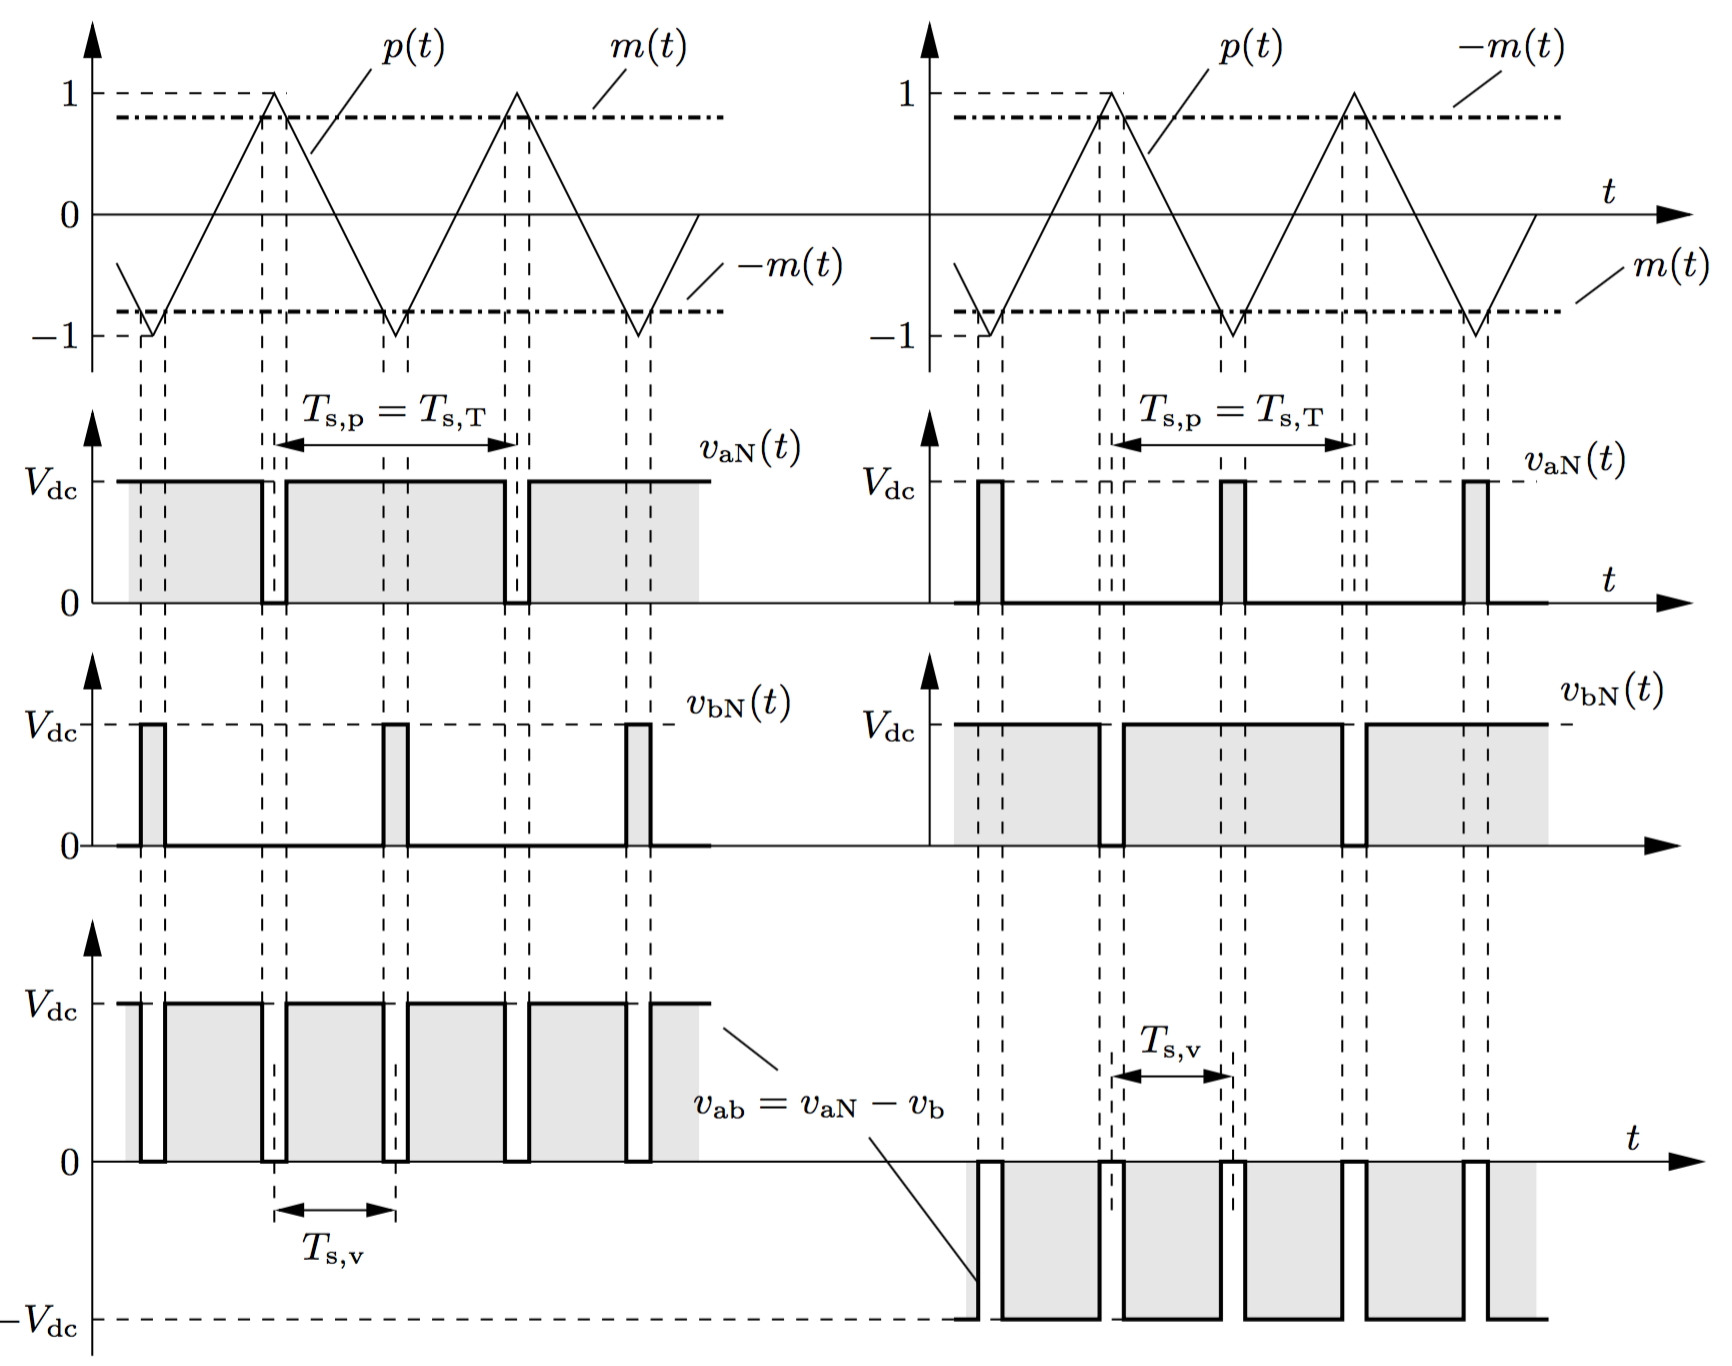
\includegraphics[scale=0.20]{ch4/11}
		\captionof{figure}{}
		\end{wrapfigure} 
		To determine what this function should be, let's go to the velocity profile in the pipe where we started from to be guided from the curves. These are more or less flat depending on the Reynolds number whith $u/u_c \rightarrow 1$ ($u_c$ velocity at the center of the pipe). Let's imagine that we plot now $1-\frac{\langle u \rangle}{u_c} = \Delta u /u_c$ in function of $y/R$, 1 will become 0 and  $0 \rightarrow 1$, the graph will be reversed (\autoref{fig:4.12} left). The curves seems to be similar, so maybe I take the velocity deficit of the half hight $\Delta u(0.5)/u_c$ which depends on Reynolds number and plot that for $\frac{u_c - \langle u \rangle}{u_c}\frac{u_c}{\Delta u}$ (\autoref{fig:4.12} center). When this = 1, $y/r = 0.5$ and we see that it fall on the same curve as \autoref{fig:4.12} left but we get a single curve. This means that 
		\begin{equation}
			\frac{u - \langle u \rangle}{\Delta u} = f\left(\frac{y}{R}\right)
		\end{equation}
		where the only scale that doesn't appear based on \eqref{eq:4.46} is $u_\tau$. So if we plot $\frac{u_e  - \langle u \rangle}{u_\tau} = f\left(\frac{y}{R}\right)$ ($u_e$ max velocity at the center) we will obtain a single curve shown on \autoref{fig:4.12} right. 
\begin{figure}[h]
\begin{center}
      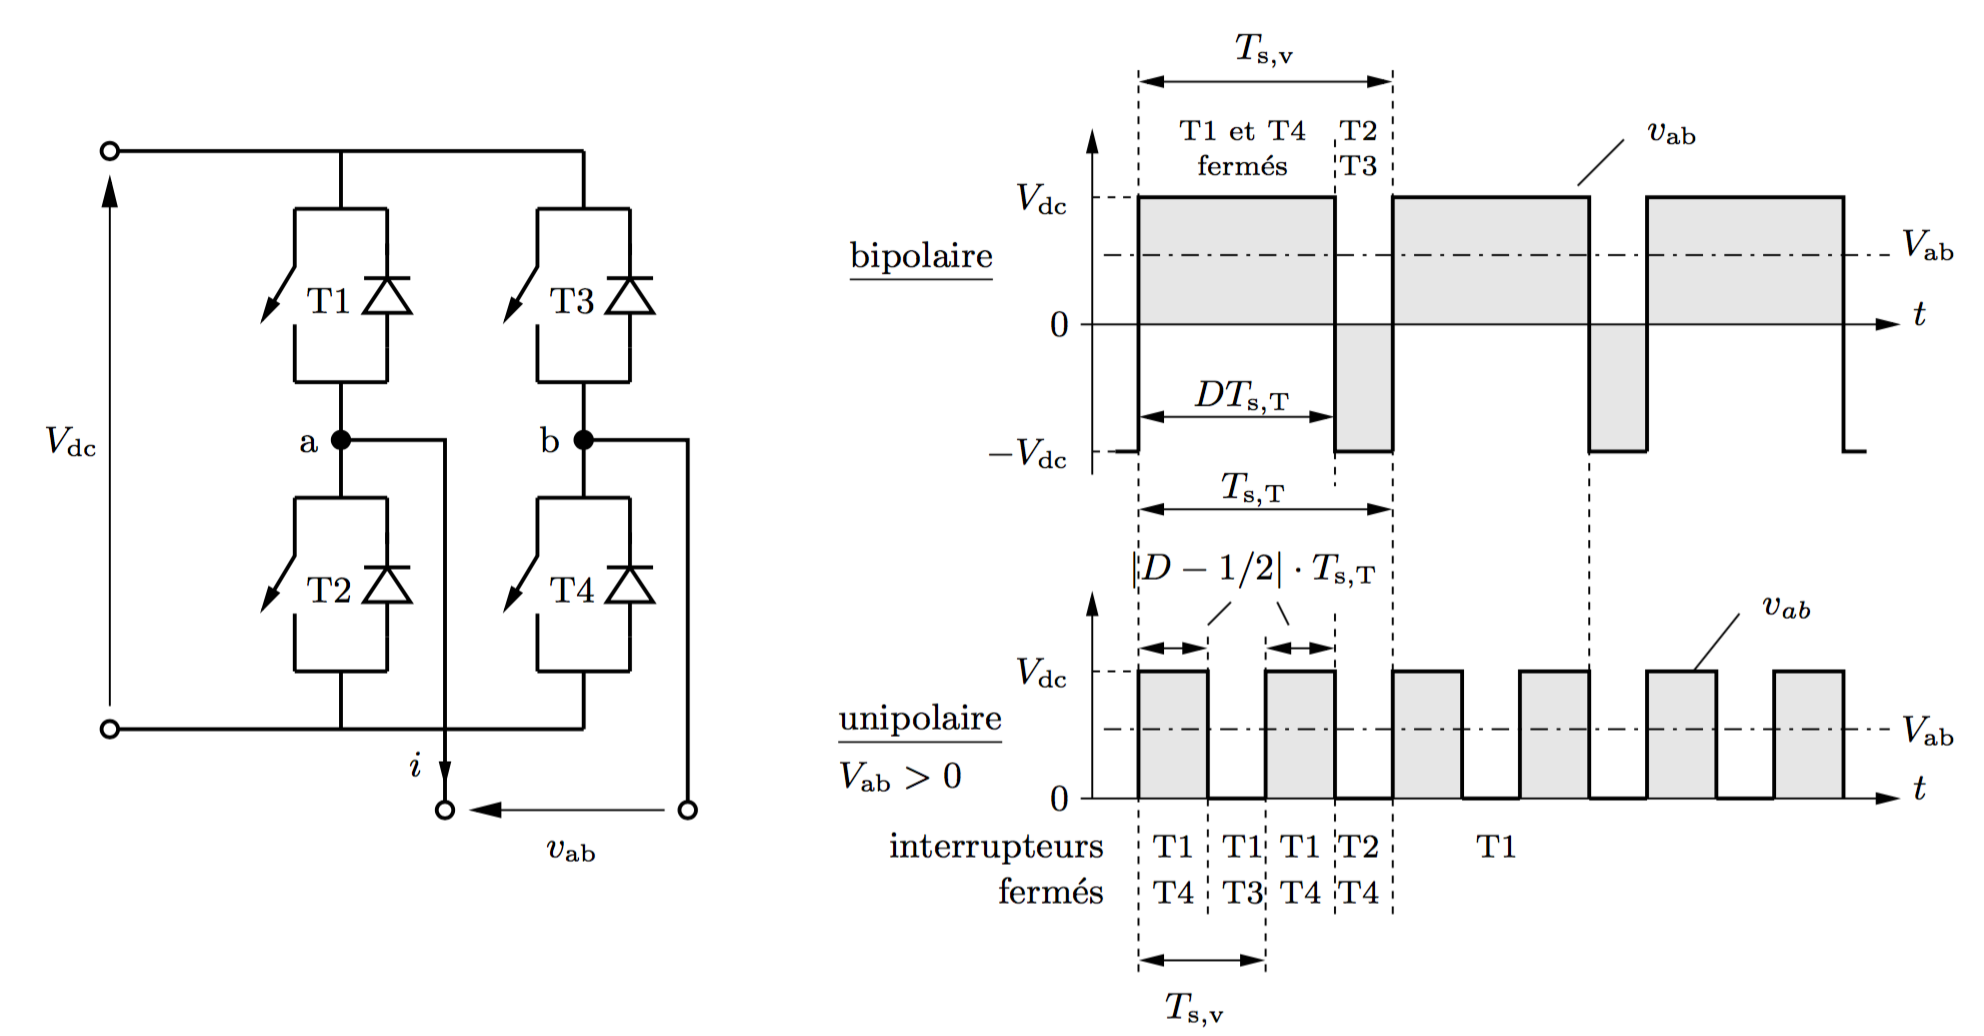
\includegraphics[scale=0.19]{ch4/12} \quad  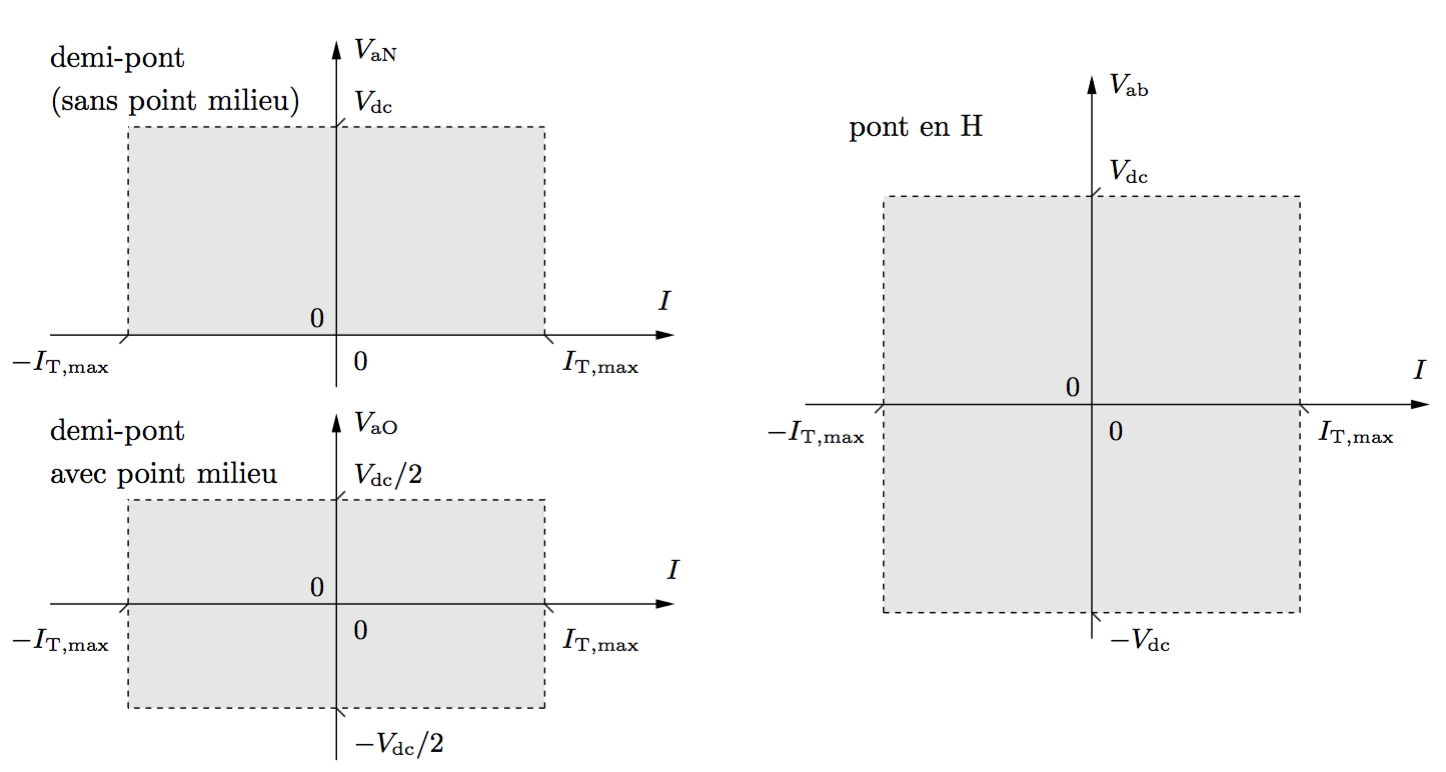
\includegraphics[scale=0.185]{ch4/13} \quad 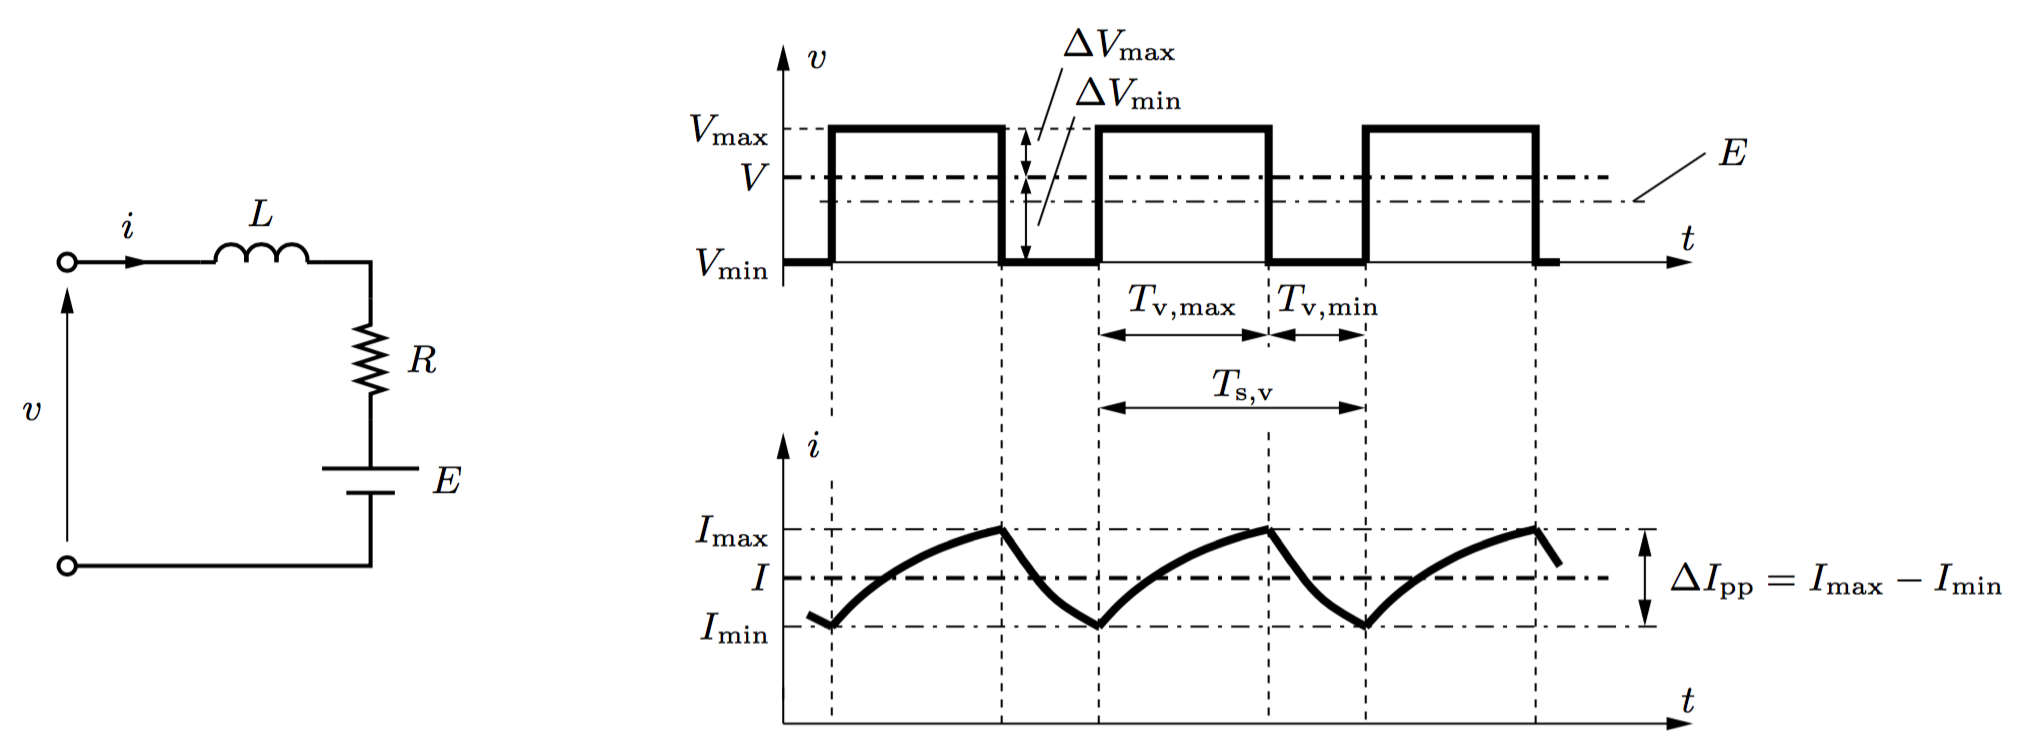
\includegraphics[scale=0.24]{ch4/14}
\captionof{figure}{}
\label{fig:4.12}
\end{center}
\end{figure}

		Interestingly enough, the logarithmic low is compatible with the outer scaling 
		\begin{equation}
			\frac{\langle u \rangle }{u_\tau} = u^+ = \frac{1}{k}\ln y^+ + B
		\end{equation}
		But what's $u_e /u_\tau$? We know that 
		\begin{equation}
			u_\tau = \sqrt{\frac{\tau _{wall}}{\rho}} \qquad \Rightarrow \frac{u_\tau}{u_e} = \sqrt{\frac{\tau _{wall}}{\rho u_e^2}} = \sqrt{\frac{C_f}{2}} \qquad \Rightarrow \frac{u_e}{u_\tau} = \sqrt{\frac{2}{C_f}} 
		\end{equation}
		where we define the \textbf{friction coefficient} $C_f = \frac{\tau _{wall}}{\rho u_e^2 /2}$ as we defined the pressure coefficient $\frac{p-p_\infty}{\rho \uinf ^2 /2}$. By combining the two last equation, we have
		\begin{equation}
		\begin{aligned}
			\frac{u_e - \langle u \rangle}{u_\tau} &= \sqrt{\frac{2}{C_f}} - \frac{1}{\kappa} \ln \left(\frac{yu_\tau}{\nu}\frac{\delta}{\delta}\right) - B = \sqrt{\frac{2}{C_f}} - \frac{1}{\kappa} \ln \frac{\delta u_\tau}{\nu} - B -\frac{1}{\kappa} \ln \frac{y}{\delta}\\
			&= cst -\frac{1}{\kappa} \ln \frac{y}{\delta}
		\end{aligned}		
		\end{equation}

		\begin{wrapfigure}[10]{l}{5.5cm}
		\vspace{-5mm}
		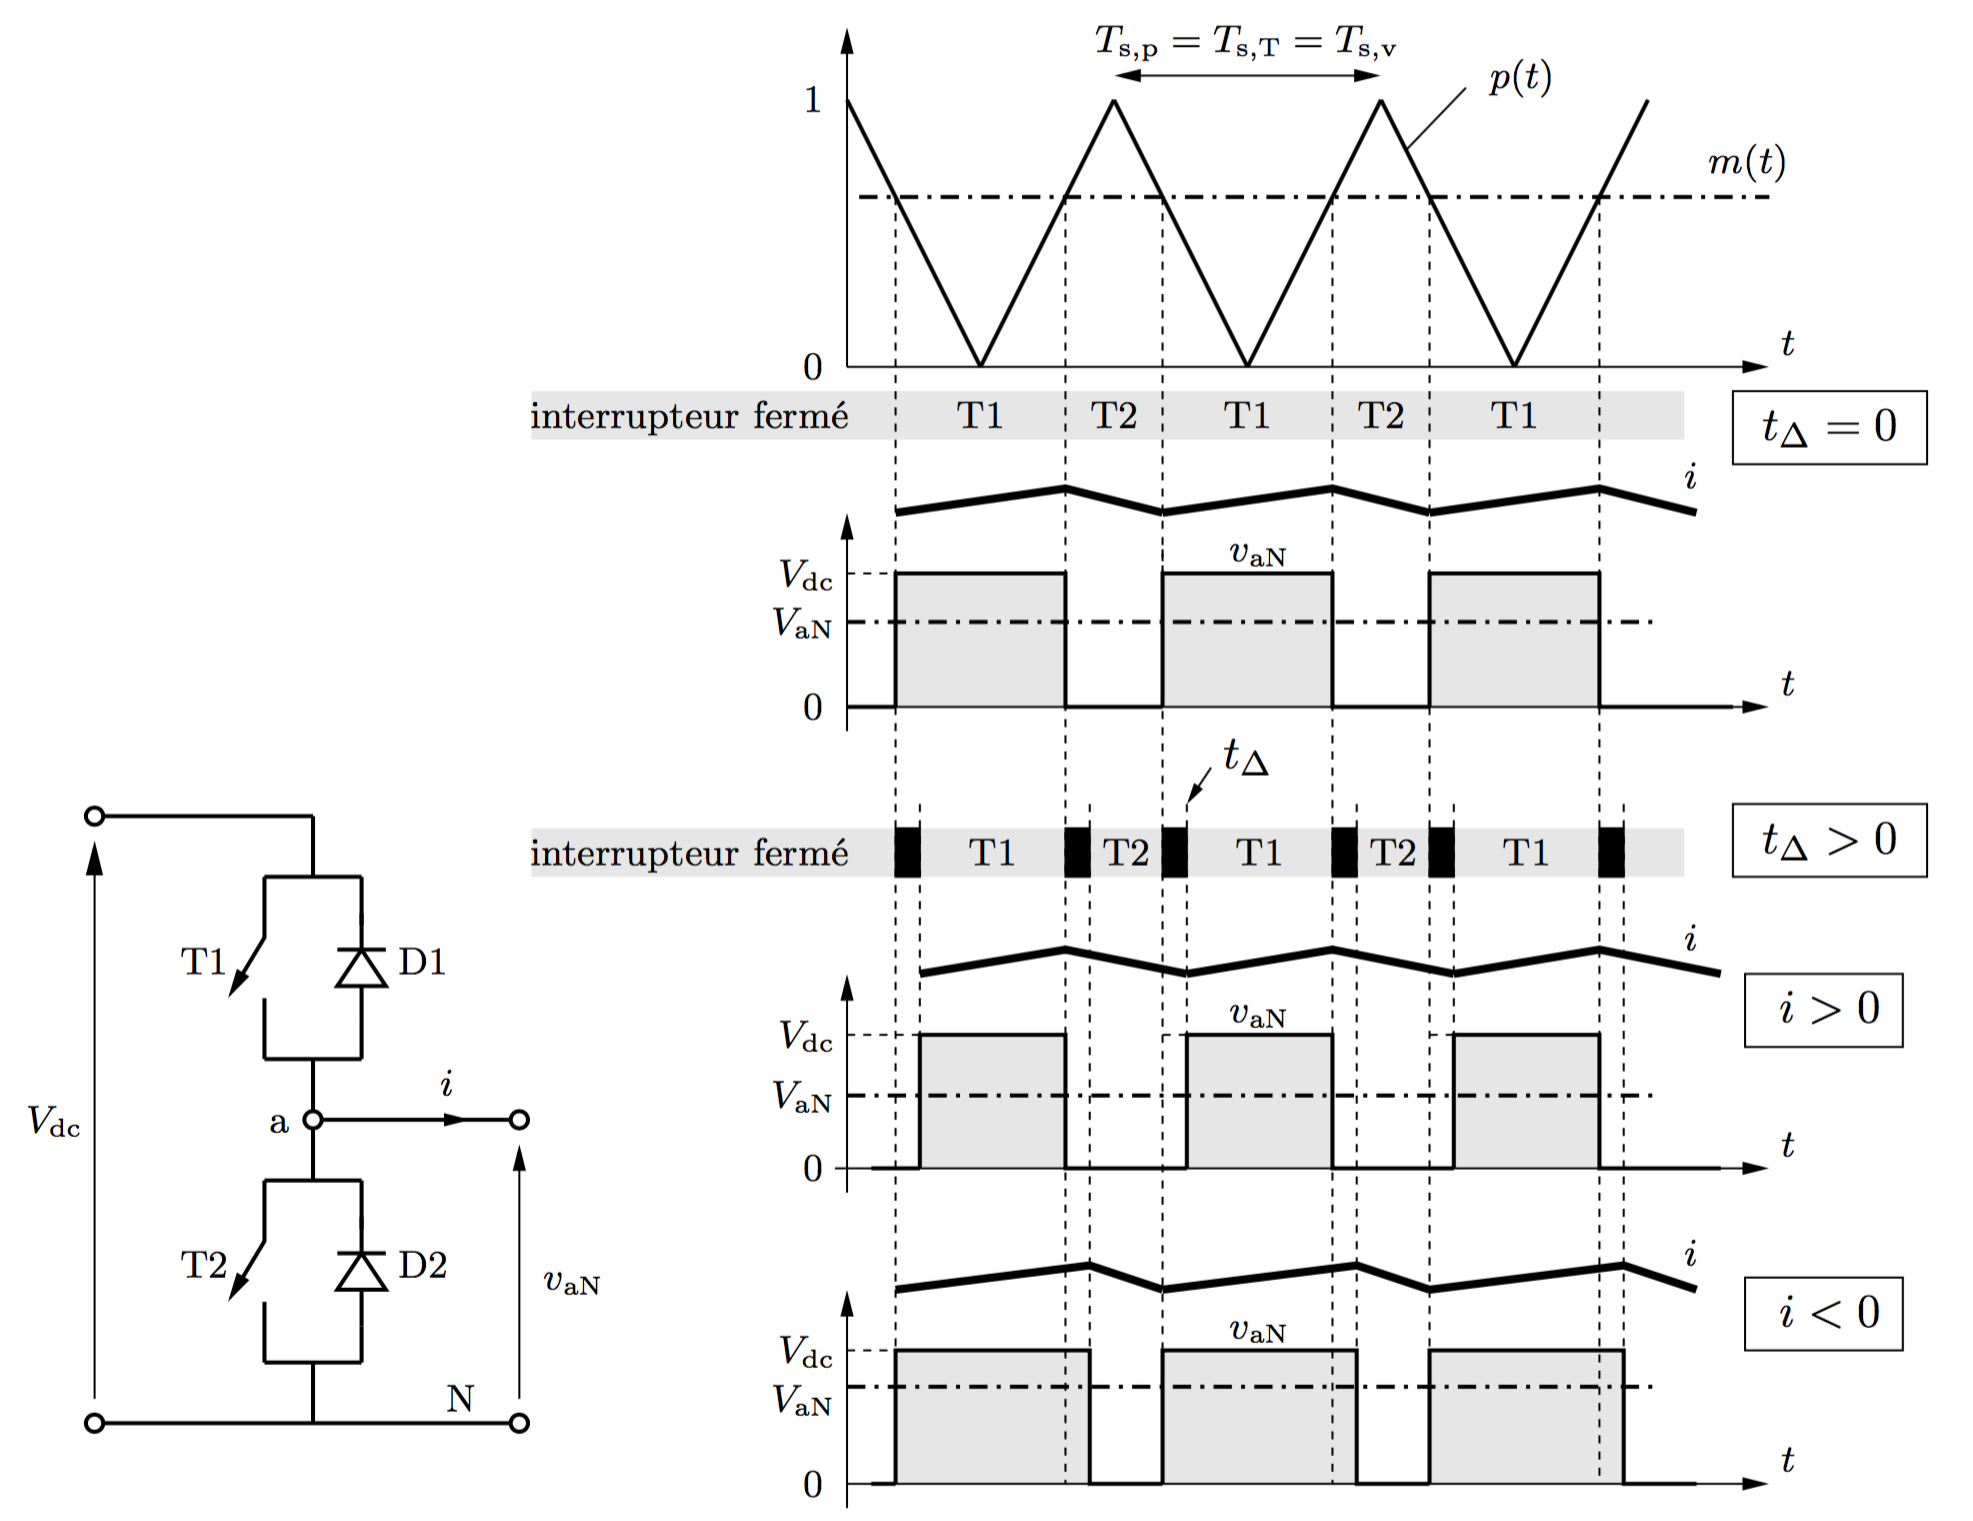
\includegraphics[scale=0.25]{ch4/15}
		\captionof{figure}{}
		\label{fig:4.13}
		\end{wrapfigure} 
		that confirms the previously founded relation. Wa can plot this in logarithmic scale that gives \autoref{fig:4.13}. We see that it obbeys the logarithmic law as in the overlap layer which is compatible with the inner and outer zone scaling. In fact we can rewrite our last equation as 
		\begin{equation}
			 \frac{u_e - \langle u \rangle}{u_\tau} = f\left( \frac{y}{\delta}\right) = cst -\frac{1}{\kappa} - g\left(\frac{y}{\delta} \right)
		\end{equation}
		where $g\left(\frac{y}{\delta} \right)$ is the deviation compared to the logarithmic law. Because of velocity deficit = 0 when $y/\delta =1$, it turns out that the cst = g(1). As conclusion, we found that the velocity profile is given by 
		\begin{equation}
			u^+ = \frac{1}{\kappa} \ln y^+ + B + g\left(\frac{y}{\delta} \right)
		\end{equation}
 		and this is observed on \autoref{fog:4.8} where we observe the deviation at the very right side of the figure. 
 		
 		\begin{wrapfigure}[9]{r}{5.4cm}
		\vspace{-5mm}
		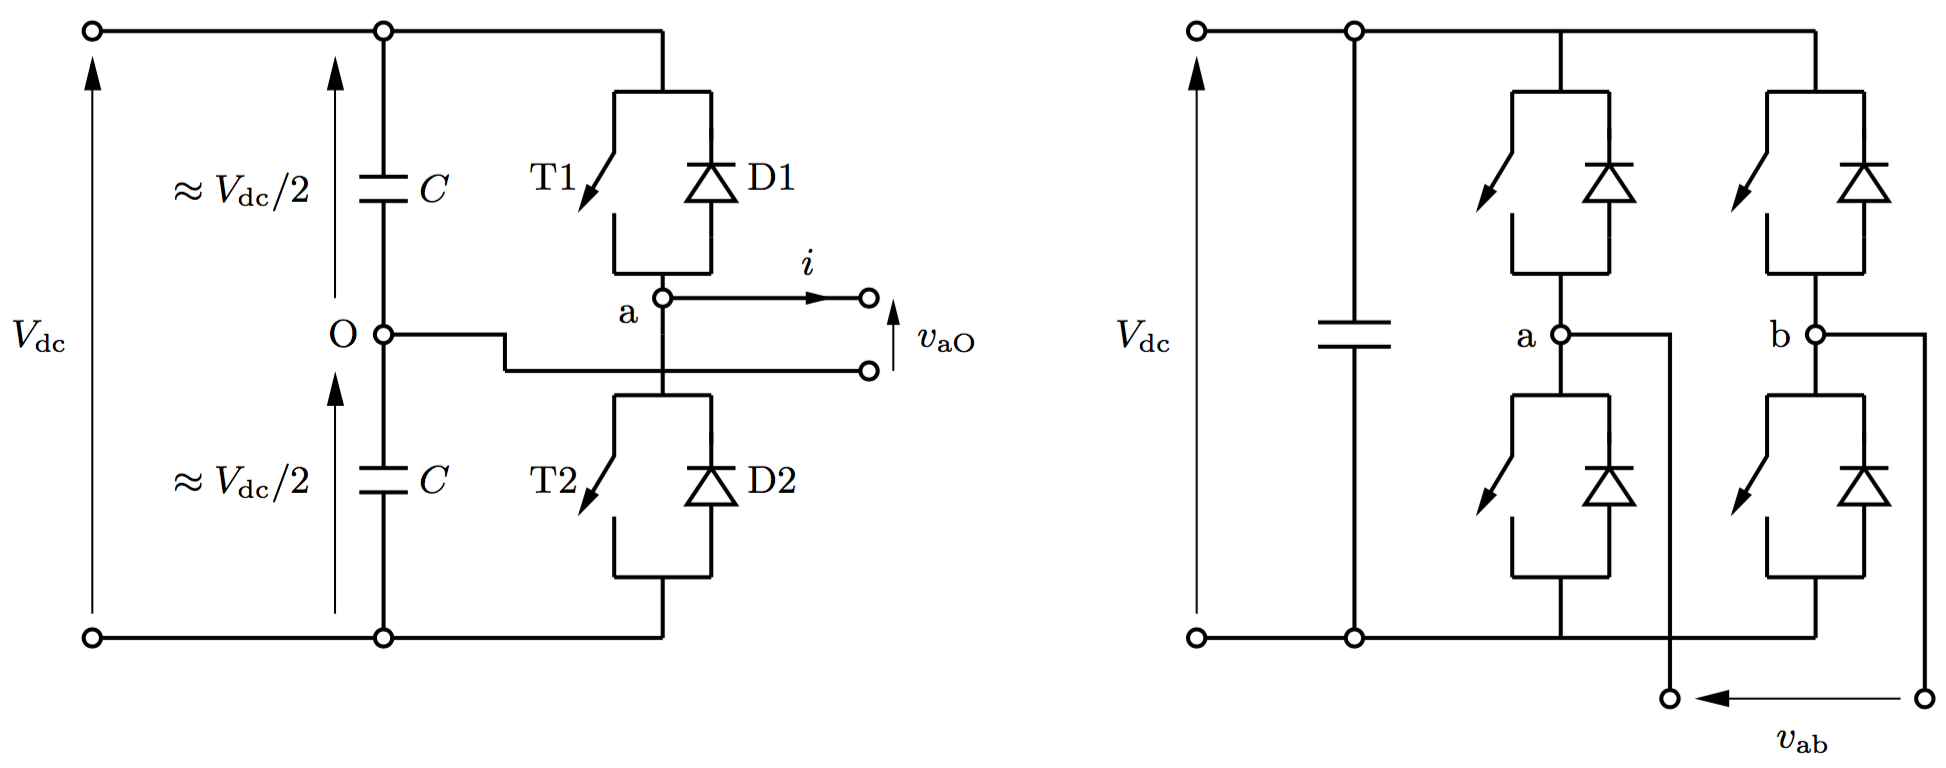
\includegraphics[scale=0.4]{ch4/16}
		\captionof{figure}{}
		\label{fig:4.16}
		\end{wrapfigure} 
		For the case of zero pressure gradient, Coles observed that the deviation from the logarithmic velocity profile $g\left(\frac{y}{\delta} \right)$ is similar to the velocity profile in a half-jet
or wake
\begin{equation}
	g\left(\frac{y}{\delta} \right) = \Pi(x)w \left(\frac{y}{\delta} \right) \approx \Pi(x)2\sin ^2 \left(\frac{\pi}{2}\frac{y}{\delta} \right) 
\end{equation}
      which was subsequently called the \textbf{law of the wake}. The coefficient $\Pi (x)$ is the amplitude of the wake, which varies slightly with Reynolds number as shown on Fig. 29, ultimately reaching a constant value equal to about 0.55 for $Re\theta > 5000.$
      
     \newpage
\section{Introduction to turbulent modelling}
	Let's remind the average Navier-Stokes equation 
	\begin{equation}
		\rho \left[ \frac{\partial \bar{u}_i}{\partial t} + \frac{\partial \overline{u_i u_j}}{\partial x_j} \right] = - \frac{\partial \bar{p}}{\partial x_i} + \frac{\partial }{\partial x_j} \Big[ \underbrace{\mu \ \left( \frac{\partial \bar{u}_i}{\partial x_j} + \frac{\partial \bar{u}_j}{\partial x_i} \right)}_{\tau^v_{ij}} - \underbrace{\rho \bar{u_i}' \bar{u_j}'}_{\tau_{ij}^t} \Big]
	\end{equation}
	There is still some unknowns, we will try to find equations describing these unknowns. It is possible, but the problem is that we introduce more unknowns than we had before, it doesn't solve the problem. This means that to close the system of equation, one of them has to stop at one stage and model the unkonown terms. One approach is to model directly the Reynold stresses as a function of the average flow quantities, this is called \textbf{first order closure approach}.  The other strategy is to retain the transport equations  for Reynolds stresses and to model the unknows in these equations, \textbf{second order closure model}. We will make an introduction with the first approach. The most corresponding method to this is Bousinesq approach or Eddy viscosity approach. The idea is to use a model analogous to viscous stresses. For these we have the \textbf{Newton's model} that says 
	\begin{equation}
		\tau _{ji} = \mu\big( \frac{\D u_i}{\D x_j} + \frac{\D u_j}{\D x_i}  \underbrace{- \frac{2}{3}\delta _{ij}\frac{\D u_k}{\D x_k}}_{=0 \mbox{ constant density}} \big) 
		\Rightarrow  - \rho \bar{u}_i' \bar{u}_j' = \mu_t \left( \frac{\partial \bar{u}_i}{\partial x_j} + \frac{\partial \bar{u}_j}{\partial x_i} \right) - \rho \underbrace{\overline{u'_k u'_k}}_{2k} \frac{\delta _{ij}}{3}  
		\label{eq:4.55}
	\end{equation}
	where $\mu _t$ is the \textbf{Eddy viscosity coefficient} and where we needed to add the last term in the second expression because if we consider the trace of $- \rho \bar{u_i}' \bar{u}_j'$, so if we contract $i$ and $j$ which gives $\overline{(u'_1)^2 + (u'_2)^2 + (u'_3)^2} \neq 0$ that can be seen as twice the \textbf{fluctuation kinetic energy} $\mathbf{2k}$ while $2\frac{\D u_i}{\D x_i} = 0$. This is one more unknown but we know that 
	\begin{equation}
		\frac{\D }{\D w_j} \left(-\rho \frac{2k}{3}\delta _{ij} \right) = \frac{\D}{\D x_i}\left(- \frac{2}{3} \rho k\right) \qquad \Rightarrow - \frac{\D}{\D x_i}\left( p  +\frac{2}{3} \rho k \right)
	\end{equation}
	This is add to the pressure gradient because it has the same form and is an effective pressure. The only unknown is now the viscosity to model the 6 unknowns of the Reynolds stresses. Contrary to $\mu$ which is only function of the the fluid thermodynamic state, $\mu_t = f$(fluid properties, average flow field quantities, space coordinates) and varies within the flow. The simpliest model to find it is an algebric model 
	
	\subsubsection{Algebric model}
		It uses some physical intuition and dimentional analysis. We know that $\mu _t = \rho \nu _t$ and $[\nu _t] = L^2T^{-1}$. So we need a caracteristic fluctuation length scale and time scale. We will describe the \textbf{Prandtl’s Mixing Length Model} which says, for
		\begin{equation}
			T^{-1} : \qquad \frac{\D \bar{u}}{\D y}
		\end{equation}
		and for the length scale, we take the average distance travelled by the fluctuating particle, this is clear that this distance is limited by the wall. This leads Prandtl to consider 
		\begin{equation}
			L = \kappa y \qquad \Rightarrow \mu _t = \rho (\kappa y)^2 \frac{\D \bar{u}}{\D y}.
		\end{equation}
		We will now see an application of this for the average velocity profile in the overlap layer \autoref{fig:4.7}. We remind that 
		\begin{equation}
			\tau _{xy}^{tot} (y) = \tau _{xy}^{V} (y)  + \tau _{xy}^{R} (y) \approx \tau _{wall}
		\end{equation}
		we will assume that the total stress is essentialy the stress at the wall. We know that Reynolds stress is dominant in this region which is given by Eddy model \eqref{eq:4.55}
		\begin{equation}
		\begin{aligned}
			&\tau _{wall} = \tau _{xy}^R (y) = \mu_t \frac{\D \bar{u}}{\D y} = \rho (\kappa y)^2 \left(\frac{\D \bar{u}}{\D y}\right)^2 \qquad \Rightarrow \frac{\tau _{wall}}{\rho} = (\kappa y)^2 \left(\frac{\D \bar{u}}{\D y}\right)^2\\
			&\Rightarrow \frac{\D \bar{u}}{\D y} = \frac{u _\tau}{\kappa y} \qquad \Rightarrow \frac{\D u^+}{\D y^+} = \frac{1}{\kappa y} \qquad \Rightarrow u^+ = \frac{1}{\kappa}\ln y^+ + B
		\end{aligned}
		\end{equation}
		and this is consistant with the universal logarithmic profile in the overlap layer. For the buffer layer, $\mu _t$ is too large, so it's not accurate. So the mixing length has to be reduced near the wall. A popular model for this is the Van Dreast dampings 
		\begin{equation}
			l(y) = \left( 1 - \log \left( -\frac{y^+}{A^+} \right) \right) \kappa y = \left( 1 - \exp \left( -\frac{yu_\tau}{26 \nu} \right) \right) \kappa y 
		\end{equation}
		where $A^+ = 26$. This is a good approximation for mixing length in the buffer layer. 
\chapter{La polarisation}
\section{État de polarisation}
On se rappelle que la notion d'onde est dérivée des équations de Maxwell
\begin{equation}
\rot\rot\vec{\mathcal{E}} = -\mu_0\epsilon_0\dfrac{\partial^2\vec{\mathcal{E}}}{\partial t^2}\qquad\Leftrightarrow
\qquad \Delta\mathcal{E}= \mu_0\epsilon_0\dfrac{\partial^2\mathcal{E}}{\partial t^2}
\end{equation}
où l'on a considéré une équation scalaire et non vectorielle par facilité : $\mathcal{E} = \mathcal{E}_x
,\mathcal{E}_y, \mathcal{E}_z$. Cette équation possède une solution d'onde plane 
\begin{equation}
\mathcal{E} = Ee^{ikz}e^{-i\omega t} + c.c.
\end{equation}
où on a considéré l'axe $z$ et où l'on n'a pas utilisé pour une fois les phaseurs mais une autre approche disant 
que le champ \textbf{réel}\footnote{Car on rajoute le complexe conjugué.} $\mathcal{E}$ n'est que le champ écrit 
sous forme de phaseur additionné à son complexe conjugué, c.c. Sous forme vectorielle
\begin{equation}
\vec{\mathcal{E}} = (E_x\vec{1_x}+E_y\vec{1_y}+E_z\vec{1_z})e^{ikz}e^{-i\omega t} + c.c.
\end{equation}
où les $E_i\in\mathbb{C}$ (ceci permet d'avoir un déphasage entre les composantes du champ). On sait que
\begin{equation}
\div \vec{\mathcal{E}} = ikE_z e^{ikz}e^{-i\omega t} = 0\qquad\Rightarrow\qquad E_z=0
\end{equation}

	\begin{wrapfigure}[11]{r}{3.5cm}
	\vspace{-5mm}
	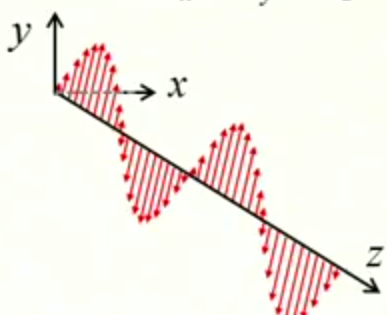
\includegraphics[scale=0.23]{ch5/image1.png}
	\captionof{figure}{ }
	\end{wrapfigure}
Une onde électromagnétique est dite \textit{transverse}
\begin{equation}
\hookrightarrow \vec{\mathcal{E}} = (E_x\vec{1_x}+E_y\vec{1_y})e^{ikz}e^{-i\omega t} + c.c.
\end{equation}
On observe bien sur le schéma ci-contre que l'amplitude possède une composante selon $x$ et $y$ : il 
s'agit d'une polarisation \textit{linéaire}.

	\subsection{Évolution du champ électrique d'une onde plane}
	Reprenons l'onde plane transverse se déplaçant le long de l'axe $z$
	\begin{equation}
	\vec{\mathcal{E}} = (E_x\vec{1_x}+E_y\vec{1_y})e^{ikz}e^{-i\omega t} + c.c.
	\end{equation}
	où $E_i\in\mathbb{C}$ : on peut les réécrire sous une forme polaire
	\begin{equation}
	E_x = \frac{1}{2}A_x e^{i\phi_x},\qquad\qquad E_y = \frac{1}{2}A_x e^{i\phi_y}
	\end{equation}
	où le facteur $1/2$ permet de faire apparaître un cosinus. 	Après substitution 
	(\danger\ ne pas oublier le c.c. sinon pas de cosinus et $\mathcal{E}\notin\mathbb{R}$ !)
	\begin{equation}
	\mathcal{E}_x = \frac{1}{2}A_x e^{i(kz-\omega t\phi_x)} + c.c.,\qquad\Leftrightarrow\qquad 
	\mathcal{E}_x = A_x\cos(kz-\omega t +\phi_x)
	\end{equation}
	On obtient similairement
	\begin{equation}
	\left\{\begin{array}{lll}
	\mathcal{E}_x &= A_x\cos(kz-\omega t +\phi_x) &= A_x\cos(\alpha)\\
	\mathcal{E}_y &= A_y\cos(kz-\omega t +\phi_y) &= A_y\cos(\alpha+\underbrace{\phi_y-\phi_x}_{\delta})\\
	\end{array}\right.
	\end{equation}
	
	\begin{wrapfigure}[9]{r}{4.5cm}
	\vspace{-9mm}
	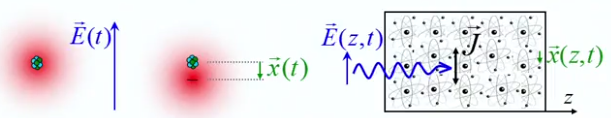
\includegraphics[scale=0.4]{ch5/image2.png}
	\captionof{figure}{ }
	\end{wrapfigure}
	Ceci représente une évolution du champ électrique, pas spécialement évidente à décrire. 
	En les traçant et en les sommant, on retrouve ci-contre pour $\phi_i=0$, l'évolution linéaire 
	(en pointillé ci-contre). 
	Si l'on considère $\phi_x\neq0,\phi_y=0$, il faut "reculer" le cosinus sur l'axe $z$ : on 
	a bien une avance de phase en $x$ (en trait plein ci-contre) et le champ ne s'annule plus nul 
	part.\\
	
	\begin{wrapfigure}[9]{l}{4cm}
	\vspace{-5mm}
	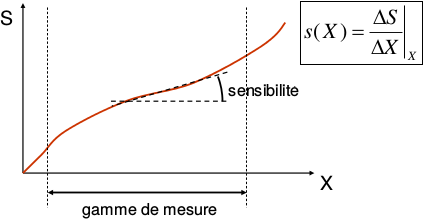
\includegraphics[scale=0.6]{ch5/image3.png}
	\captionof{figure}{ }
	\end{wrapfigure}	
	Pour se simplifier, posons que l'argument du cosinus dans l'expression de $\mathcal{E}_x$ est 
	$\alpha$ : il représente la distance parcourue sur l'axe $z$ si le temps est fixé, à une 
	constante près. Pour un $z$ donné, $\alpha$ représente le temps avec un signe moins et toujours 
	à une constante près. Prenons comme premier exemple, un déphasage nul $\delta = \phi_y-\phi_x=0$.
	Cherchons le lien entre $\mathcal{E}_x$ et $\mathcal{E}_y$ en effectuant le rapport suivant
	\begin{equation}
	\dfrac{\mathcal{E}_y}{\mathcal{E}_x} = \dfrac{A_y}{A_x}\qquad\Rightarrow\qquad \mathcal{E}_y = 
	\dfrac{A_y}{A_x}\mathcal{E}_x
	\end{equation}
	Cette linéarité est représentée ci-dessus. Les flèches représentent "l'oscillation" du champ 
	électrique. Il s'agit encore une fois de la \textit{polarisation linéaire} qui est caractérisée 
	par une certaine amplitude et un certain angle par rapport à l'axe.\\
	
	Considérons un autre exemple : $\delta=\phi_y-\phi_x=\frac{\pi}{2}$, soit un quart de période 
	de l'évolution des composantes. Cette situation ne donne aucun nœud, le champ ne s'annule plus.
	En substituant $\delta$
	\begin{equation}
	\left\{\begin{array}{ll}
	\mathcal{E}_x &= A_x\cos(\alpha)\\
	\mathcal{E}_y &= -A_y\sin(\alpha)
	\end{array}\right.
	\end{equation}
	En éliminant $\alpha$ de cette évolution paramétrique du champ, nous obtenons le lieu des points 
	qu'occupera le champ électrique :
	
 	\begin{wrapfigure}[5]{r}{3.2cm}
	\vspace{-5mm}
	\includegraphics[scale=0.5]{ch5/image4.png}
	\captionof{figure}{ }
	\end{wrapfigure}	
	\begin{equation}
	\left(\frac{\mathcal{E}_x}{A_x}\right)^2+\left(\frac{\mathcal{E}_y}{A_y}\right)^2 = 1
	\end{equation}
	
	Il s'agit de l'équation d'une ellipse. Reste à savoir comment le champ agit dynamiquement : 
	dans quel sens "tourne-t-on" sur cette ellipse. Rappelons-nous : $\alpha = kz-\omega+\phi_x$. On 
	s'intéresse à la composante temporelle : si $z=\phi_x=0$, $\alpha \propto -t$. Quand le temps 
	évolue, on observe une diminution progressive de la composante en $x$ à partir de 1 et le comportement 
	inverse pour le composante en $y$, ayant un sinus. Le point de départ est 1 pour le cosinus et 0 
	pour le sinus, la rotation se fera dans le sens trigonométrique positif. Si l'on applique la 
	règle de la main droite pour déterminer la direction de l'axe $z$, les doigts vont dans le même 
	sens que la rotation sur l'ellipse : il s'agit d'une \textit{polarisation elliptique droite}.\\
	
 	\begin{wrapfigure}[7]{r}{5.5cm}
	\vspace{-5mm}
	\includegraphics[scale=0.5]{ch5/image5.png}
	\captionof{figure}{ }
	\end{wrapfigure}	
	Regardons ceci géométriquement, en représentant les vecteurs résultants en bleu. On remarque 
	que si on effectue la règle de la main droite, en $z$, il tourne dans l'autre sens (le pouce 
	est opposé à l'axe $z$). C'est normal, l'évolution temporelle d'une onde progressive est inversée 
	par rapport à se composante spatiale. Un polarisation est dite \textit{droite} lorsqu'elle tourne 
	dans le sens horlogique lorsqu'on s'éloigne en $z$ : le sens de rotation en $z$ sera opposé à 
	sa rotation en $t$.\\
	
	Si $A_x=A_y$, on obtient une \textit{polarisation circulaire droite}. Si on considère $\delta = 
	-\frac{\pi}{2}$ on se trouve dans le cas d'un retard de phase. Le champ est spatialement 
	dextrogyre : il faut inverser le sens de la polarisation est alors dit \textit{gauche} (avec la
	règle de la main gauche, on obtiendrait l'axe $z$, petit moyen mnémotechnique).\\
	
	Cessons-en maintenant avec les exemples et considérons le cas général. Pour se faire, effectuons
	$\cos(a+b)$ dans l'expression $\mathcal{E}_y$
	\begin{equation}
	\frac{\mathcal{E}_x}{A_y} = \underbrace{\cos\alpha}_{\mathcal{E}_x/A_x}\cos\delta-\sin\alpha\sin\delta
	\end{equation}
	où l'on utilise la première expression (celle de $\mathcal{E}_x$) et le fait que $\DS \sin\alpha = 
	\sqrt{1-\left(\frac{\mathcal{E}_x}{A_x}\right)}$. On trouve alors
	\begin{equation}
	\frac{\mathcal{E}_y}{A_y} = \frac{\mathcal{E}_x}{A_x}\cos\delta -\sqrt{1-\left(\frac{\mathcal{E}_x}{
	A_x}\right)^2}\sin\delta
	\end{equation}
	N'ayant plus de $\alpha$, il s'agit bien du lieu des points de l'extrémité du vecteur du champ électrique. 
	Analysons ceci en commençant par passer la racine à gauche et en élevant tout au carré
	\begin{equation}
	\sqrt{1-\left(\frac{\mathcal{E}_x}{A_x}\right)^2}\sin\delta = \frac{\mathcal{E}_x}{A_x}\cos\delta -
	\frac{\mathcal{E}_y}{A_y} 
	\end{equation}
	Dès lors, en effectuant le produit remarquable
	\begin{equation}
	\left[1-\left(\frac{\mathcal{E}_x}{A_x}\right)\right]\sin^2\delta = \left(\frac{\mathcal{E}_x}{A_x}\right)^2
	\cos^2\delta +\left(\frac{\mathcal{E}_y}{A_y}\right)^2- 2\frac{\mathcal{E}_x\mathcal{E}_y}{A_xA_y}\cos\delta
	\end{equation}
	En simplifiant l'identité fondamentale trigonométrique
	\begin{equation}
	\sin^2\delta = \left(\frac{\mathcal{E}_x}{A_x}\right)^2
	+\left(\frac{\mathcal{E}_y}{A_y}\right)^2- 2\frac{\mathcal{E}_x\mathcal{E}_y}{A_xA_y}\cos\delta
	\end{equation}
	
		\begin{wrapfigure}[2]{r}{4.5cm}
	\vspace{-12mm}
	\includegraphics[scale=0.5]{ch5/image6.png}
	\captionof{figure}{ }
	\end{wrapfigure}
	Il s'agit de l'équation d'une conique qui n'est rien d'autre qu'une ellipse. Il s'agit du cas de 
	polarisation le plus général portant le doux nom d'\textit{ellipse de polarisation}. Celle-ci aura 
	une certaine inclinaison $\psi$ repérée par rapport à l'axe $x$. Sans rentrer dans les détails, on 
	peut montrer que
	\begin{equation}
	\psi = \frac{1}{2}\arctan\left[\dfrac{2A_xA_y}{A_x^2-A_y^2}\cos\delta\right]
	\end{equation}
	La différence avec les secondaires et qu'à la place d'utiliser $a$ et $b$ pour le grand/petit axe, 
	on utilise l'ellipticité $\chi$ donné par (non démontré ici)
	\begin{equation}
	\chi = \frac{1}{2}\arcsin\left[\dfrac{2A_xA_y}{A_x^2+A_y^2}\sin\delta\right]
	\end{equation}
	L’ellipse de polarisation, et donc l'état de polarisation, sera décrite par son inclinaison et 
	son ellipticité. Par construction $\chi=\arctan(b/a)$ où $|b|<a$ (si $b>0$ la polarisation sera 
	droite) et donc $|\chi| \leq  \frac{\pi}{4} \rightarrow \chi <0$ représente une polarisation 
	elliptique gauche.\\
	
	Prenons un exemple : $\delta = 0\rightarrow \chi = 0\rightarrow b = 0$ et l'ellipse se réduit à 
	une droite. Une ellipticité nulle indique que l'on se trouve dans le cadre d'une polarisation 
	linéaire. Pour l'inclinaison 
	\begin{equation}
	\tan(2\psi) = \left[\frac{2A_y/A_x}{1-A_y^2/A_x^2}\right] = \dfrac{2\tan\psi}{1-\tan^2\psi}
	\end{equation}
	où l'on a utilisé la formule de l'angle double. Par identification $A_y/A_x = \tan\psi$ ce qui 
	est bien le résultat précédemment obtenu.\\
	
	\begin{wrapfigure}[6]{l}{4cm}
	\vspace{-9mm}
	\includegraphics[scale=0.34]{ch5/image7.png}
	\captionof{figure}{ }
	\end{wrapfigure}
	Soif de savoir, partons sur un nouvel exemple : $\delta = \frac{\pi}{2}, A_y=A_x \rightarrow 
	\chi = \frac{\pi}{4}\rightarrow a=b=A_x$. Il s'agit de la polarisation circulaire droite, 
	$\chi$ étant positif. Pour le calcul de l'inclinaison, on obtient une indétermination ($\psi = 0/0$)
	ce qui est cohérent : l'inclinaison d'un cercle est indéterminée. La fin de la vidéo propose quelques 
	petites illustrations animées.\\
	
	Même si ces expressions sont correctes, elles sont peut utilisables en pratique. La section 
	suivante se consacre dès lors à la mesure expérimentale de la polarisation.
	
	\newpage
\section{Mesure de la polarisation}
Les mesures sur la lumières sont essentiellement des mesures de l'intensité
\begin{equation}
I = A_x^2+A_y^2
\end{equation}
Avant de voir comment mesurer ceci, intéressons-nous au lien entre $\psi$ et $\chi$. Nous avions
\begin{equation}
\left\{\begin{array}{ll}
\psi &= \frac{1}{2}\arctan\left[\dfrac{2A_xA_y}{A_x^2-A_y^2}\cos\delta\right]\\
\chi &= \frac{1}{2}\arcsin\left[\dfrac{2A_xA_y}{A_x^2+A_y^2}\sin\delta\right]	
\end{array}\right.
\end{equation}
En manipulant ces expressions (en faisant surtout l'effort de le faire), il est possible de 
ré-exprimer $A_x$ (en remplaçant l'expression de $I$ dans $\chi$). De même pour $A_y$
cccc
En élevant ces deux expressions au carré on retrouve bien les deux relations suivantes 
\begin{equation}
\left\{\begin{array}{ll}
I &= A_x^2+A_y^2\\
A_x^2-A_y^2 &= I\cos(2\chi)\cos(2\psi)
\end{array}\right.
\end{equation}
Les angles doubles apparaissant dans cette dernière expression justifie l'utilité de 
l'utilisation de $\chi$.

	\subsection{Sphère de Poincaré}
	Ces relations remarquables faisant intervenir les angles $\psi$ et $\chi$ a donné l'idée à 
	Poincaré de représenté les états de polarisation sous la forme d'un point sur une sphère. 
	
	\begin{center}
	\includegraphics[scale=0.30]{ch5/image8.png}
	\captionof{figure}{ }
	\end{center}
	
	Un point sur cette sphère est repéré à partir de deux angles : $2\psi$ comme angle polaire et 
	$2\chi$ comme angle azimutal. On pourrait croire que le facteur 2 est limitant, mais ce n'est 
	pas le cas car pour un angle $\chi>180^\circ$ on retrouve les mêmes états.\\
	
	\begin{wrapfigure}[5]{l}{3.64cm}
	\vspace{-9mm}
	\includegraphics[scale=0.34]{ch5/image9.png}
	\captionof{figure}{ }
	\end{wrapfigure}
	L'intérêt de cette représentation vient de George Stokes : il a proposé de représenté l'état 
	de polarisation, soit un point de la sphère de Poincaré, en terme de coordonnées dans un système 
	cartésien à l'aide des paramètres de Stokes $S_1, S_2$ et $S_3$. La sphère de Poincaré est donc 
	maintenant décrite dans ce repère cartésien. Notons que cette sphère a pour rayon l'intensité de 
	la lumière émise et bien qu'il n'est pas nécessaire à la caractérisation de la polarisation, 
	c'est toujours utile de l'avoir. On désigne l'intensité avec le paramètre de Stokes $S_0$.
 	\begin{equation}
 	S_0 = I
 	\end{equation}
 	Le premier paramètre de Stokes est la coordonnée $S_1$ qui est obtenue en projetant le "vecteur 
 	intensité" dans le plan horizontal $S_1S_2$ puis en effectuant la projection sur $S_1$ (\danger\ 
 	l'angle $\chi$ n'est pas exactement défini comme les coordonnées polaires). En faisant de même 
 	pour $S_2$ et $S_3$, on obtient les \textit{paramètres de Stokes}
 	\begin{equation}
	\left\{\begin{array}{ll}
	S_0 &= I\\
 	S_1 &= I\cos(2\chi)\cos(2\psi)\\
 	S_2 &= I\cos(2\chi)\sin(2\psi)\\
 	S_3 &= I\sin(2\chi)
	\end{array}\right.
 	\end{equation}
 	Il est évident que la somme des composantes au carrée va donner la norme au carrée du vecteur 
 	intensité, étant dans un repère cartésien
 	\begin{equation}
 	S^2_1+S^2_2+S^2_3 = S^2_0
 	\end{equation}
	On peut maintenant revenir à nos deux expressions précédentes
	\begin{equation}
	\left\{\begin{array}{ll}
	A_x &= \sqrt{\frac{I}{2}}[1+\cos(2\chi)\cos(2\psi)]^{\frac{1}{2}}\\
	A_y &= \sqrt{\frac{I}{2}}[1-\cos(2\chi)\cos(2\psi)]^{\frac{1}{2}}
	\end{array}\right.
	\end{equation}
	Et on va voir que des regroupements vont être possibles avec les paramètres de Stokes. 
 	\begin{equation}
	\left\{\begin{array}{lll}
	S_0 &= I&\qquad\rightarrow S_0 = A_x^2+A_y^2\\
 	S_1 &= I\cos(2\chi)\cos(2\psi)&\qquad\rightarrow S_1 = A_x^2-A_y^2\\
 	S_2 &= I\cos(2\chi)\sin(2\psi)&\qquad\rightarrow S_2 = 2A_xA_y\cos\delta\\
 	S_3 &= I\sin(2\chi)&\qquad\rightarrow S_3 = 2A_xA_y\sin\delta
	\end{array}\right.
 	\end{equation}
 	Les démonstrations ne sont pas données ici, mais il suffit de partir des expressions de 
 	ci-dessus et faire un peu d'algèbre.
 	
 		\subsubsection{Illustration}
 		Considérons quelques exemples pour s'habituer à ce nouveau formalisme. Regardons la 
 		situation aux deux pôles : $S_1=S_2=0$. On peut directement en tirer que
 		\begin{equation}
 		A_x = A_y,\qquad\qquad \delta = \pm\frac{\pi}{2}
 		\end{equation}
		Comme $A_x=A_y$, $S_3 = 2\underbrace{A_xA_y}_{\pm I}\sin\delta = \pm I$ en utilisant 
		l'expression $S_0 = A_x^2+A_y^2 = 2A_x = I$. En en tire $\chi = \pm \frac{\pi}{4}$. 
		Comme nous avons une indétermination sur $\psi$ (dans l'expression de $S_2$, peu 
		importe sa valeur tout est vérifié) il s'agit bien d'un état de polarisation circulaire. \\
		
		Autre exemple : à l'équateur $S_3=0 \rightarrow \chi = 0 \rightarrow \delta = 0\rightarrow 	
		2A_xA_y=I\sin(2\psi)$. Avec $S_1$ : $A_x^2-A_y^2 = I\cos(2\psi)$. En faisant le rapport des 
		deux, on retrouve $\tan(2\psi)=\frac{2A_xA_y}{A_x^2-A_y^2}$, c'est bien la polarisation 
		linéaire précédemment rencontrée.
		
	\subsection{Mesure de l'état de polarisation}
	Imaginons qu'une lumière ai une certaine polarisation et qu'il est nécessaire de la déterminer 
	la polarisation. Nous allons pouvoir tout déterminer, à l'aide de quatre étapes 
	\begin{enumerate}
	\item \textit{Étape "0"}\\
	Il suffit de mesurer l'intensité de la lumière
	\begin{equation}
	I_0 = A_x^2+A_y^2 = S_0
	\end{equation}
	\item \textit{Étape "1"}\\
	Il faut préalablement insérer un polarisateur mis en polarisation horizontale. Se faisant, 
	nous récupérons l'intensité en $x$, $I_1=A_x^2$. 
	\begin{center}
	\includegraphics[scale=0.50]{ch5/image11.png}
	\captionof{figure}{ }
	\end{center}	
	Avec cette mesure, il est possible d'effectuer 
	une manipulation intéressante
	\begin{equation}
	I_0-I_1 = A_y^2
	\end{equation}
	En peut en déduire $S_1$
	\begin{equation}
	\hookrightarrow S_1 = I_1(I_0-I_1) = 2I_1-I_0
	\end{equation}
	\item \textit{Etape "2"}\\
	Cette étape consiste à incliner le polariseur à 45$^\circ$. Il est important de bien comprendre 
	ce qui se passe dans le polariseur : la vibration $\mathcal{E}_x$ incidente peut être vue comme 
	la combinaison d'une vibration dans l'axe perpendiculaire à l'axe du polariseur  et une vibration 
	parallèle à cette axe (principe de superposition). 
	\begin{center}
	\includegraphics[scale=0.50]{ch5/image12.png}
	\captionof{figure}{ }
	\end{center}		
	La vibration perpendiculaire à l'axe du polariseur 
	se fait absorbé par celui-ci, seule la composante parallèle à l'axe passera dont l'intensité sera 
	$\frac{1}{\sqrt{2}}$ (car 45$^\circ$)  de celle incidente. Un raisonnement similaire peut être tenu 
	pour $\mathcal{E}_y$. On mesurera alors
	\begin{equation}
	I_2 = \left|\dfrac{1}{\sqrt{2}}A_xe^{i\phi_x}+\dfrac{1}{\sqrt{2}}A_ye^{i(\phi_x+\delta)}\right|^2 = 
	|A_x + A_y(\cos\delta +i\sin\delta)|^2
	\end{equation}
	où on a supprimé tous les termes "semblables". En effectuant le module carré
	\begin{equation}
	A_x^2+2A_xA_y\cos\delta + A_y^2\cos^2\delta + A_y^2\sin^2\delta  
	\end{equation}
	On trouve alors
	\begin{equation}
	I_2 = \frac{1}{2}\left[A_x^2+A_y^2+2A_xA_y\cos\delta\right]\quad \Rightarrow\quad 2I_2 = 
	I_0+S_2
	\end{equation}
	où les $1/2$ vient des $1/\sqrt{2}$. Finalement
	\begin{equation}
	S_2 = SI_2 - I_0
	\end{equation}
	\item \textit{Étape "3"}\\
	Pour obtenir le dernier paramètre, il est nécessaire d'introduire une lame quart d'onde. Il 
	s'agit d'une lame biréfringente : il possède deux indices de réfraction en fonction de la 
	direction. Une composante accumulera une certaine phase causant ici un déphasage entre nos 
	deux composantes du champ électrique. 
	\begin{center}
	\includegraphics[scale=0.50]{ch5/image13.png}
	\captionof{figure}{ }
	\end{center}	
	Au départ d'un déphasage nul (polarisation linéaire) 
	on obtient  un déphasage $\phi_y-\phi_x=-\frac{\pi}{2}$ (soit $\lambda/4$, d'où le nom).  
	Ceci correspond à une polarisation circulaire gauche. En terme de mesure, il faut tenir 
	compte de ce déphasage supplémentaire
	\begin{equation}
	I_3 = \left|\dfrac{1}{\sqrt{2}}A_xe^{i\phi_x}+\dfrac{1}{\sqrt{2}}A_ye^{i\left(\phi_x+\delta-
	\frac{\pi}{2}\right)}\right|^2 = |A_x + A_y(-i\cos\delta +\sin\delta)|^2
	\end{equation}
	En calculant le module carré
	\begin{equation}
	|A_x + A_y(-i\cos\delta +\sin\delta)|^2 = A_x^2+2A_xA_y\sin\delta + A_y^2\sin^2\delta +A_y^2
	\cos^2\delta
	\end{equation}
	Avec l'identité trigonométrique fondamentale, on trouve
	\begin{equation}
	I_3 = \frac{1}{2}[A_x^2+A_y^2+2A_xA_y\sin\delta]
	\end{equation}
	où l'on voit apparaître le paramètre $S_3$. On obtient alors
	\begin{equation}
	S_3 = 2I_3-I_0
	\end{equation}
	\end{enumerate}
	Nous voyons que ces quatre étapes permettent d'accéder facilement de façon expérimentales à ces 
	paramètres de Stokes. Ceci n'est que une des multiples techniques possible pour mesurer une 
	polarisation : une autre technique - directement inspirée de celle-ci - sera vue en séance de 
	laboratoire. Le gros désavantage de cette méthode est que le placement d'un polariseur provoque 
	tout de même une atténuation en $x$. Il faudrait quelque peu corriger ces mesures : il existe 
	d'autres moyen de caractériser la polarisation, ce que nous aurons l'occasion de voir plus tard.
	
	
\newpage
\section{Formalisme de Jones}
Ce formalisme se base sur la représentation complexe du champ électrique
\begin{equation}
\vec{\mathcal{E}} = (E_x\vec{1_x}+E_y\vec{1_y})e^{ikz}e^{-i\omega t} + c.c.\qquad\text{où }\ E_x = 
\frac{1}{2}A_xe^{i\phi_x},\quad E_y = \frac{1}{2}A_ye^{i\phi_y}
\end{equation}
Le premier terme n'est en réalité par vraiment un phaseur. De plus, on remarque que l'amplitude 
$E_i$ n'est que la moitié de l'amplitude réelle. Ce choix de notation a été fait pour se rapprocher 
de la littérature scientifique, mais rien n'empêche d'utiliser les fameux phaseurs
\begin{equation}
\underline{\vec{\mathcal{E}}} = (\underline{E_x}\vec{1_x}+\underline{E_y}\vec{1_y})e^{ikz}e^{-i\omega t}\qquad\text{où }\ \underline{E_x} = A_xe^{i\phi_x},\quad \underline{E_y} = A_ye^{i\phi_y}
\end{equation}
Si ici nous passons en phaseurs, c'est parce que le formalisme de Jones a été développé avec un 
tel outil. Lorsque l'on parle de $\underline{\vec{\mathcal{E}}}$, cela désigne bien un phaseur. Le 
champ sera alors obtenu en considérant la partie réelle de ce phaseur\footnote{C'est semblable avec 
ce que l'on faisait en ajoutant +c.c. où l'on prenait deux fois la partie réelle, d'où le facteur 
1/2 dans l'amplitude.}.\\

L'état de polarisation générale est elliptique d'inclinaison $\psi$ et d'ellipticité $\chi$. Le 
formalisme de Jones est utile d'un point de vue théorique, contrairement à la précédente section. 
Il permet de décrire d'un point de vue théorique l'évolution de la polarisation dans les systèmes 
optiques. Jones propose d'écrire le vecteur amplitude sous la forme vectorielle 
\begin{equation}
\left(\begin{array}{c}
\underline{E_x}\\
\underline{E_y}
\end{array}\right) = \left(\begin{array}{c}
A_xe^{i\phi_x}\\
A_ye^{i\phi_y}
\end{array}\right)
\end{equation}

		\begin{wrapfigure}[4]{l}{5.5cm}
	\vspace{-4mm}
	\includegraphics[scale=0.25]{ch5/image14.png}
	\captionof{figure}{ }
	\end{wrapfigure}
Il s'agit du \textit{vecteur de Jones}. Ce n'est rien d'autre qu'une notation plus compacte de 
notre vecteur en vue de bénéficier d'un formalisme matriciel : l'action d'un dispositif optique 
va pouvoir être exprimé sous forme d'une matrice
\begin{equation}
\left(\begin{array}{c}
\underline{E_x'}\\
\underline{E_y'}
\end{array}\right) = \left(\begin{array}{cc}
a & b\\
c & d
\end{array}\right)\left(\begin{array}{c}
\underline{E_x}\\
\underline{E_y}
\end{array}\right)
\end{equation}

\subsection{Matrice de Jones}
	\subsubsection{Propagation libre}
Afin d'introduire ce formalisme, commençons par un cas quelque peu trivial : la propagation libre. 
Le système optique est l'espace entre $0$ et $L$. 
\begin{center}
	\includegraphics[scale=0.35]{ch5/image15.png}
	\captionof{figure}{ }
\end{center}
La matrice de Jones sera simple : il faut utiliser 
un propagateur pour une distance $L$ sur chaque composante de notre vecteur de Jones
\begin{equation}
\left(\begin{array}{c}
\underline{E_x'}\\
\underline{E_y'}
\end{array}\right) = \left(\begin{array}{cc}
e^{ikL} & 0\\
0 & e^{ikL}
\end{array}\right)\left(\begin{array}{c}
\underline{E_x}\\
\underline{E_y}
\end{array}\right) = e^{ikL}\left(\begin{array}{cc}
1 & 0\\
0 & 1
\end{array}\right)\left(\begin{array}{c}
\underline{E_x}\\
\underline{E_y}
\end{array}\right)
\end{equation}
La matrice identité $\mathcal{I}$ montre que l'on n'a pas modifié l'état de polarisation. On retrouve 
l'état de polarisation à la sortie.

\subsubsection{Polariseur}
Considérons maintenant un polariseur horizontal. La matrice d'un tel polariseur sera la suivante
\begin{equation}
\left(\begin{array}{c}
\underline{E_x'}\\
\underline{E_y'}
\end{array}\right) = \left(\begin{array}{cc}
1 & 0\\
0 & 0
\end{array}\right)\left(\begin{array}{c}
\underline{E_x}\\
\underline{E_y}
\end{array}\right) = \left(\begin{array}{c}
\underline{E_x}\\
0
\end{array}\right)
\end{equation}
Ce résultat est évident dans le sens ou nous savons que seul la composante selon $x$ sera transmise.
	
		\subsubsection{Lame de phase}
		Une lame de phase pourrait être une lame demi ou quart d'onde. Ici, on se doute que la matrice 
		sera (vraiment juste) un peu plus compliquée.
		\begin{equation}
		\left(\begin{array}{c}
		\underline{E_x'}\\
		\underline{E_y'}
		\end{array}\right) = \left(\begin{array}{cc}
		1 & 0\\
		0 & e^{i\delta}
		\end{array}\right)\left(\begin{array}{c}
		\underline{E_x}\\
		\underline{E_y}
		\end{array}\right)= \left(\begin{array}{c}
		\underline{E_x}\\
		\underline{E_y}e^{i\delta}
		\end{array}\right)
		\end{equation}
		Rappelons que ce qui est intéressant c'est bien le déphasage entre les deux composantes 
		et non la phase à un point $z$ précis.
		
		\subsubsection{Rotation}
		La rotation de la polarisation est quelque chose d'important. Pour se faire, introduisons 
		les axes $x$ et $y$. Considérons une polarisation en $x$ et on considère un système causant 
		une rotation $\alpha$ à notre faisceau en $x$ (par exemple, un verre d'eau sucrée (du à la 
		chiralité de la molécule de sucre).
	\begin{center}
	\includegraphics[scale=0.35]{ch5/image17.png}
	\captionof{figure}{ }
\end{center}			
	 Trouvons cette matrice en étudiant des cas particuliers. 
		Nous avons une polarisation en $x$ comme entrée et comme sortie une rotation de $\alpha$
		\begin{equation}
		\left(\begin{array}{c}
		1\\
		0
		\end{array}\right),\qquad\qquad		\left(\begin{array}{c}
		\cos\alpha\\
		\sin\alpha
		\end{array}\right)
		\end{equation}
		Forcément, notre matrice doit vérifier
		\begin{equation}
			\left(\begin{array}{c}
		1\\
		0
		\end{array}\right) = \left(\begin{array}{cc}
		\cos\alpha & b\\
		\sin\alpha & d
		\end{array}\right)\left(\begin{array}{c}
		\underline{E_x}\\
		\underline{E_y}
		\end{array}\right)= \left(\begin{array}{c}
		\cos\alpha\\
		\sin\alpha
		\end{array}\right)
		\end{equation}
		où $b,d$ sont à déterminer. En considérant cette fois une polarisation verticale et la sortie
		\begin{equation}
				\left(\begin{array}{c}
		1\\
		0
		\end{array}\right),\qquad\qquad		\left(\begin{array}{c}
		-\sin\alpha\\
		\cos\alpha
		\end{array}\right)
	\end{equation}				
	Nous avons ainsi trouvé notre matrice de rotation. Dans le formalisme de Jones :
	\begin{equation}
			\left(\begin{array}{c}
		\underline{E_x'}\\
		\underline{E_y'}
		\end{array}\right) = \left(\begin{array}{cc}
	\cos\alpha & -\sin\alpha\\
	\sin\alpha & \cos\alpha
	\end{array}\right)\left(\begin{array}{c}
		\underline{E_x}\\
		\underline{E_y}
		\end{array}\right)
	\end{equation}
	
		\subsubsection{Rotation d'un élément}
		Illustrons le cas de la rotation d'une lame d'onde\footnote{Le polariseur est laissé comme 
		exercice.} Comme nous ne savons pas comment décrire une lame d'onde inclinée de $\alpha$ nous 
		allons ruser : on va redresser la lame mais tourner la polarisation dans l'autre sens. En effet, 
		entre l'axe de la lame et la polarisation se trouve un angle $-\alpha$. 
\begin{center}
	\includegraphics[scale=0.35]{ch5/image16.png}
	\captionof{figure}{ }
\end{center}		
		En redressant tout, 
		la lame va redevenir horizontale et la polarisation va tourner d'un angle $-\alpha$. Faisant 
		ceci, on pourra appliquer la matrice pour la lame de phase et obtenir une sortie. Il faut alors 
		redresser cette sortie d'un angle $\alpha$.
		\begin{center}
	\includegraphics[scale=0.35]{ch5/image18.png}
	\captionof{figure}{ }
\end{center}	
		Matriciellement, cela donne
		\begin{equation}
		\left(\begin{array}{c}
		\underline{E'}_x\\
		\underline{E'}_y
		\end{array}\right)\left(\begin{array}{cc}
	\cos\alpha & -\sin\alpha\\
	\sin\alpha & \cos\alpha
	\end{array}\right)
	\left(\begin{array}{cc}
	1 & 0\\
	0 & e^{i\delta}
	\end{array}\right)\left(\begin{array}{cc}
	\cos\alpha & \sin\alpha\\
	-\sin\alpha & \cos\alpha
	\end{array}\right)		\left(\begin{array}{c}
		\underline{E}_x\\
		\underline{E}_y
		\end{array}\right)
		\end{equation}
		Une lame inclinée d'une angle $\alpha$ est représentée par les trois matrices ci-dessus : 
		la matrice de rotation opposé $-\alpha$, la matrice de la lame suivi de la matrice de rotation de 
		l'angle de la lame, $\alpha$.\\
		
		\textsc{Illustration 1}\ \\
		Supposons que nous plaçons à la sortie d'un laser un polariseur horizontal suivi d'une 
		lame demi-onde inclinée d'un angle $\alpha$. 
		\begin{center}
	\includegraphics[scale=0.35]{ch5/image19.png}
	\captionof{figure}{ }
\end{center}			
		La polarisation induite par le polariseur 
		revient à considérer que, à l'entrée de la lame
		\begin{equation}
		\left(\begin{array}{c}
		\underline{E}_x\\
		\underline{E}_y
		\end{array}\right) = \left(\begin{array}{c}
		1\\
		0
		\end{array}\right)
		\end{equation}
		Pour une lame demi-onde, $\delta =\pi \rightarrow e^{i\pi} = -1$. Nous obtenons alors
		\begin{equation}
				\left(\begin{array}{c}
		\underline{E'}_x\\
		\underline{E'}_y
		\end{array}\right)\left(\begin{array}{cc}
	\cos\alpha & -\sin\alpha\\
	\sin\alpha & \cos\alpha
	\end{array}\right)
	\left(\begin{array}{cc}
	1 & 0\\
	0 & -1
	\end{array}\right)\left(\begin{array}{cc}
	\cos\alpha & \sin\alpha\\
	-\sin\alpha & \cos\alpha
	\end{array}\right)		\left(\begin{array}{c}
		1\\
		0
		\end{array}\right)
		\end{equation}
		Après avoir effectué les produits matriciels, nous trouvons
		\begin{equation}
		\left(\begin{array}{c}
		\underline{E'}_x\\
		\underline{E'}_y
		\end{array}\right) = \left(\begin{array}{cc}
		cos^2\alpha - \sin^2\alpha\\
		2\sin\alpha\cos\alpha
		\end{array}\right)
		\end{equation}
		En appliquant les formules trigonométrique de l'arc double, on obtient
		\begin{equation}
		\left(\begin{array}{c}
		\underline{E'}_x\\
		\underline{E'}_y
		\end{array}\right)		\left(\begin{array}{cc}
		\cos(2\alpha)\\
		\sin(2\alpha)
		\end{array}\right)
		\end{equation}
		L'effet d'une lame demi-onde sur une polarisation linéaire revient à tourner 
		celle-ci d'un angle $2\alpha$.\\
		
		
		\textsc{Illustration 2}\ \\
		Considérons cette-fois une polarisation linéaire inclinée à $45^\circ$ incidente sur 
		une lame quart d'onde verticale. Nous avons premièrement
		\begin{equation}
		\left(\begin{array}{c}
		\underline{E}_x\\
		\underline{E}_y
		\end{array}\right) = \left(\begin{array}{c}
		1/\sqrt{2}\\
		1/\sqrt{2}
		\end{array}\right)
		\end{equation}
		où ce vecteur de Jones a été normalisé. Pour une lame quart d'onde $\delta = \frac{\pi}{2}
		=i$ de sorte à obtenir
		\begin{equation}
		\left(\begin{array}{c}
		\underline{E'}_x\\
		\underline{E'}_y
		\end{array}\right)		\left(\begin{array}{cc}
		1 & 0\\
		0 & i
		\end{array}\right)\left(\begin{array}{c}
		1/\sqrt{2}\\
		1/\sqrt{2}
		\end{array}\right) = \dfrac{1}{\sqrt{2}}\left(\begin{array}{c}
		1\\
		i
		\end{array}\right)
		\end{equation}
		Rappelons-nous que les composantes du vecteur sont les amplitudes en $x$ et $y$ de notre onde :
		\begin{equation}
		\underline{\vec{\mathcal{E}}} = (\underline{E_x}\vec{1_x}+\underline{E_y}\vec{1_y})e^{ikz}e^{-i
		\omega t}
		\end{equation}
		Dans notre cas $\underline{E_x}=1$ et $\underline{E_y} = i$, ce qui donne bien un déphasage de 
		$\frac{\pi}{2}$ entre les deux champs. Ceux-ci sont donc en quadrature de phase, la polarisation 
		est circulaire droite, la phase en $y$ ayant été avancée. Le vecteur de Jones normalisé d'une 
		polarisation circulaire droite est donné par
		\begin{equation}
		\dfrac{1}{\sqrt{2}}\left(\begin{array}{c}
		1\\
		i
		\end{array}\right)
		\end{equation}
		Pour une polarisation circulaire gauche, il suffit de remplacer $i$ par $-i$, $\delta$ valant 
		$-\pi/2$.\\
		\\
		
		
		

			\begin{center}
	\includegraphics[scale=0.15]{ch5/fin}
	%\captionof{figure}{ }
\end{center}				
	
	
	
	
	
	
	
	
	
	
	
	
	
	
	
	

%%%%%%%%%%%%%%%%%
% Bibliographie %
%%%%%%%%%%%%%%%%%
%\newpage
%\chapter{Bibliographie}
%\nocite{*}
%\printbibliography[heading=none]

%%%%%%%%%%%
% Annexes %
%%%%%%%%%%%
\appendix
%\input{annexes/annexe1.tex}


\end{document}